
Here I show the full table for \autoref{fig:nn_comp}.

\begin{table}[b]
  \centering
  \resizebox*{!}{\textheight}{%
  \begin{tabular}{r||cccc}
    \hline \\
    & Neural network - 26 & SVM - polynomial & Neural network 5+3 & SVM - radial \\
    \hline \\
    &
    \begin{subfigure}[b]{0.2\textwidth}
      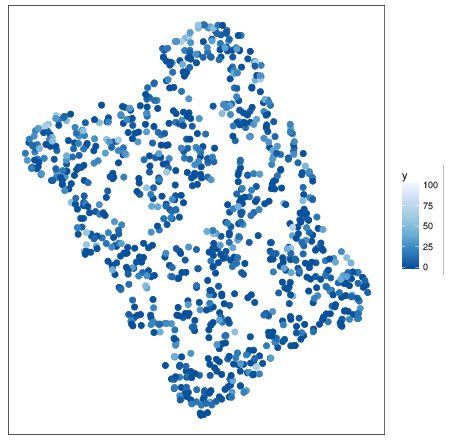
\includegraphics[width=\textwidth]{boston_nn_26_sp.png}
    \end{subfigure}
    &
    \begin{subfigure}[b]{0.2\textwidth}
      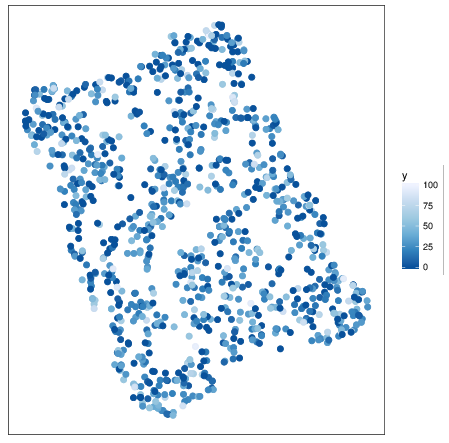
\includegraphics[width=\textwidth]{boston_svm_poly_sp.png}
    \end{subfigure}
    &
    \begin{subfigure}[b]{0.2\textwidth}
      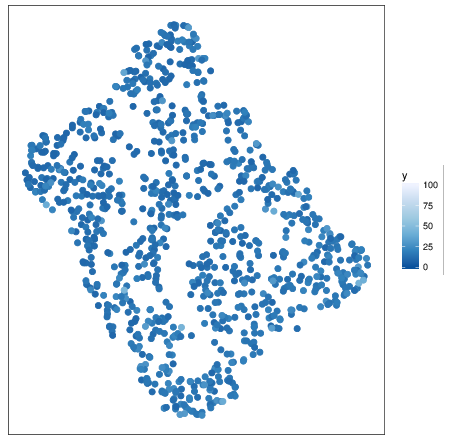
\includegraphics[width=\textwidth]{boston_nn_5x3_sp.png}
    \end{subfigure}
    &
    \begin{subfigure}[b]{0.2\textwidth}
      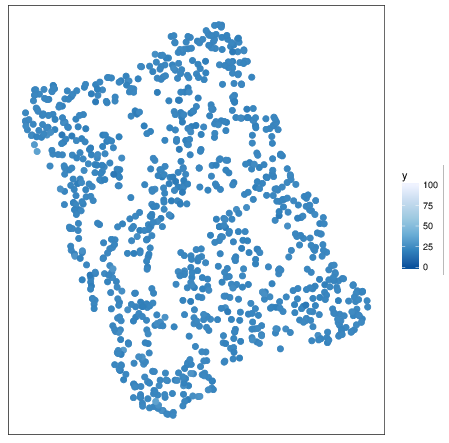
\includegraphics[width=\textwidth]{boston_svm_radial_sp.png}
    \end{subfigure} 
    \\
    \hline \\
    Per capita crime rate &
    \begin{subfigure}[b]{0.2\textwidth}
      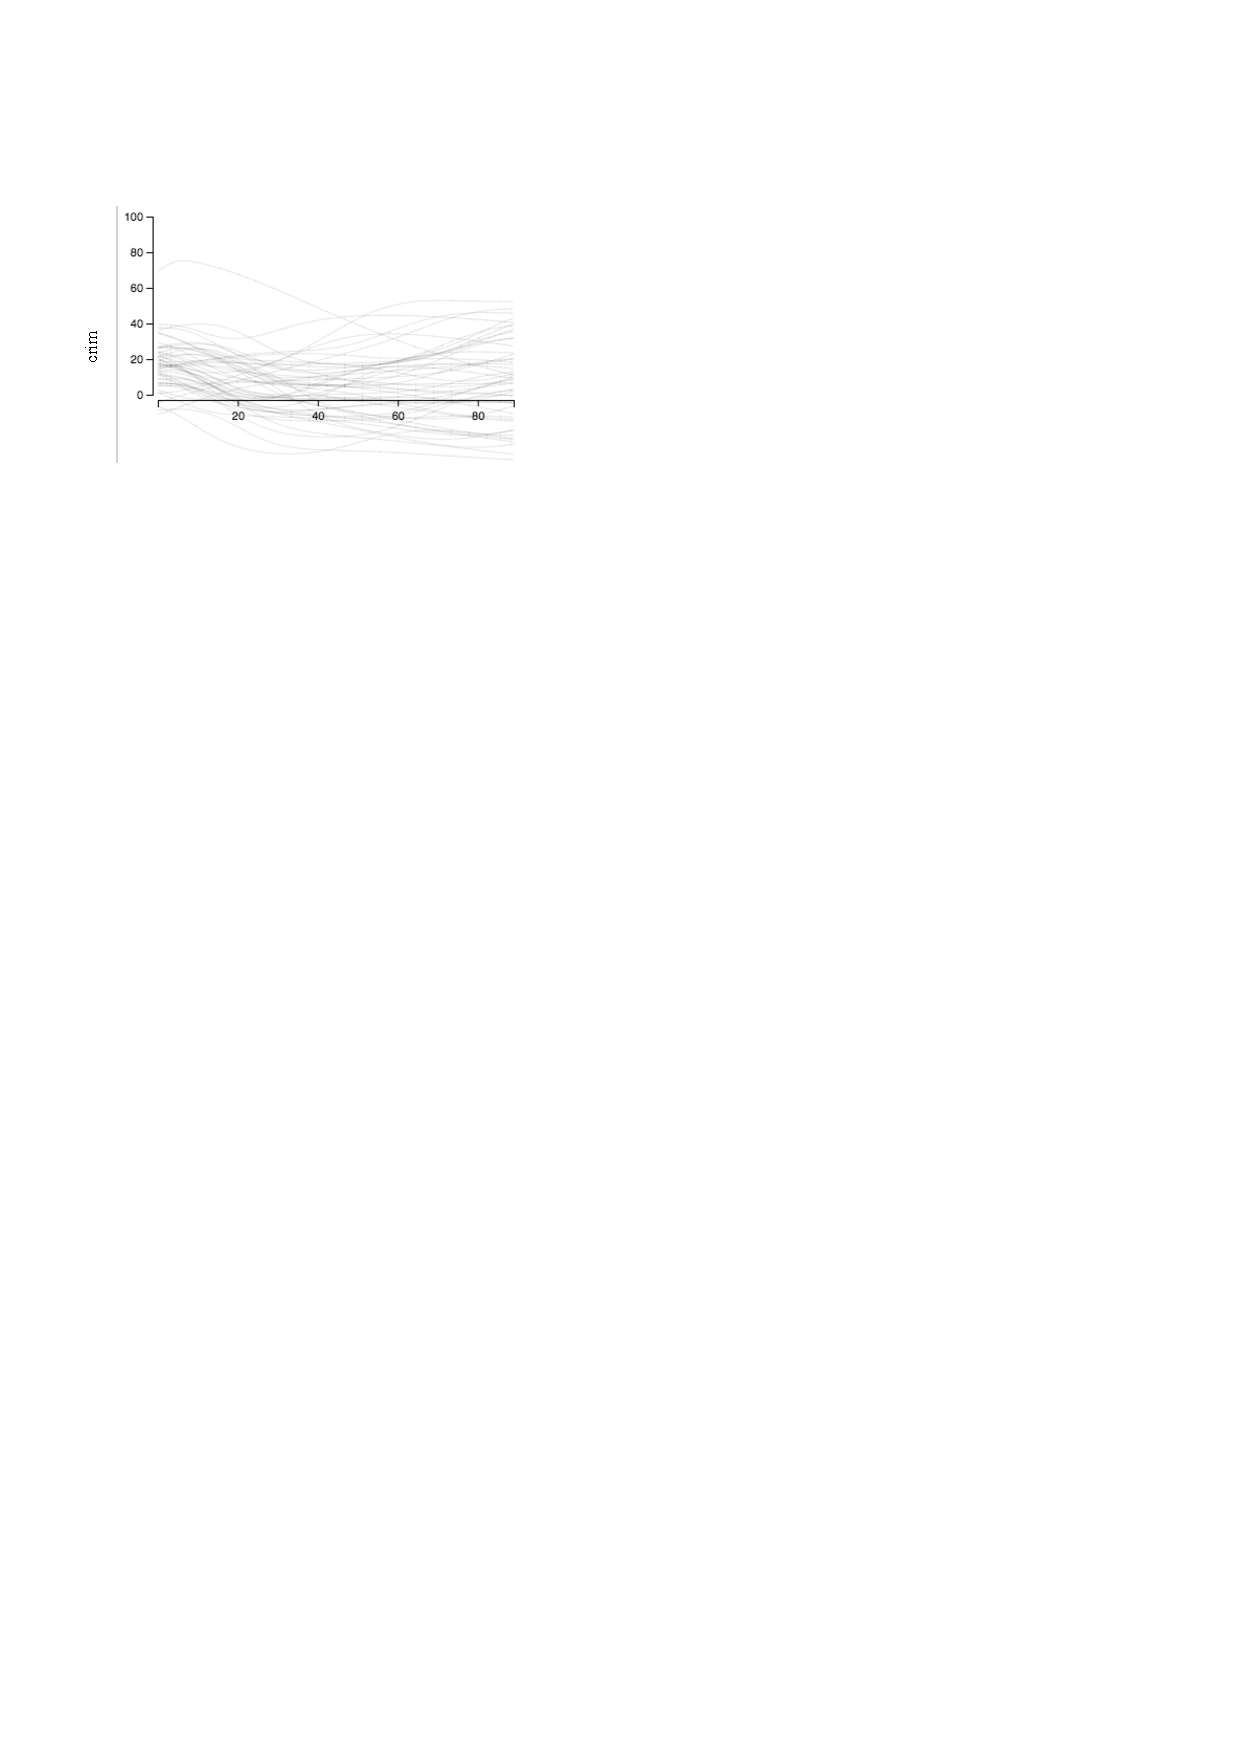
\includegraphics[width=\textwidth]{nn26_1.pdf}
    \end{subfigure}
    &
    \begin{subfigure}[b]{0.2\textwidth}
      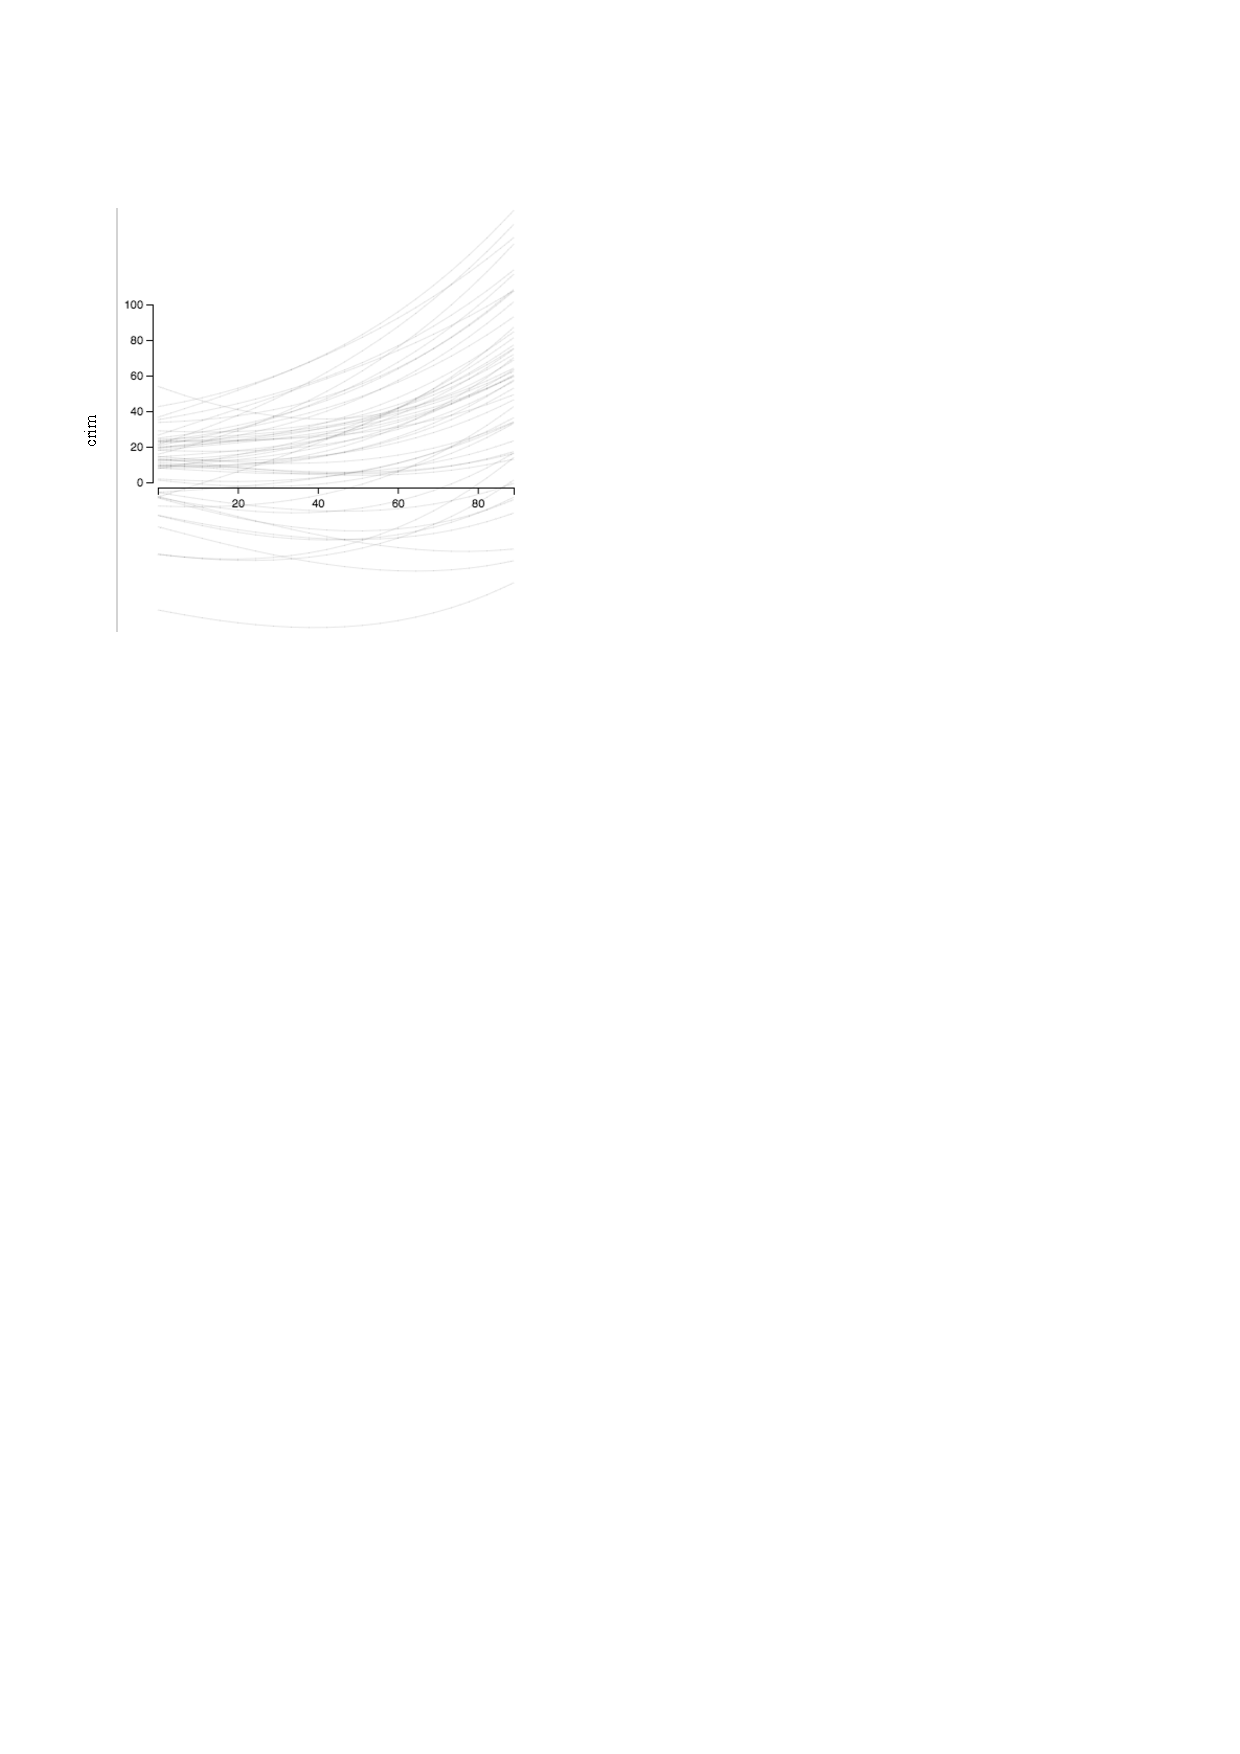
\includegraphics[width=\textwidth]{svmp_1.pdf}
    \end{subfigure}
    &
    \begin{subfigure}[b]{0.2\textwidth}
      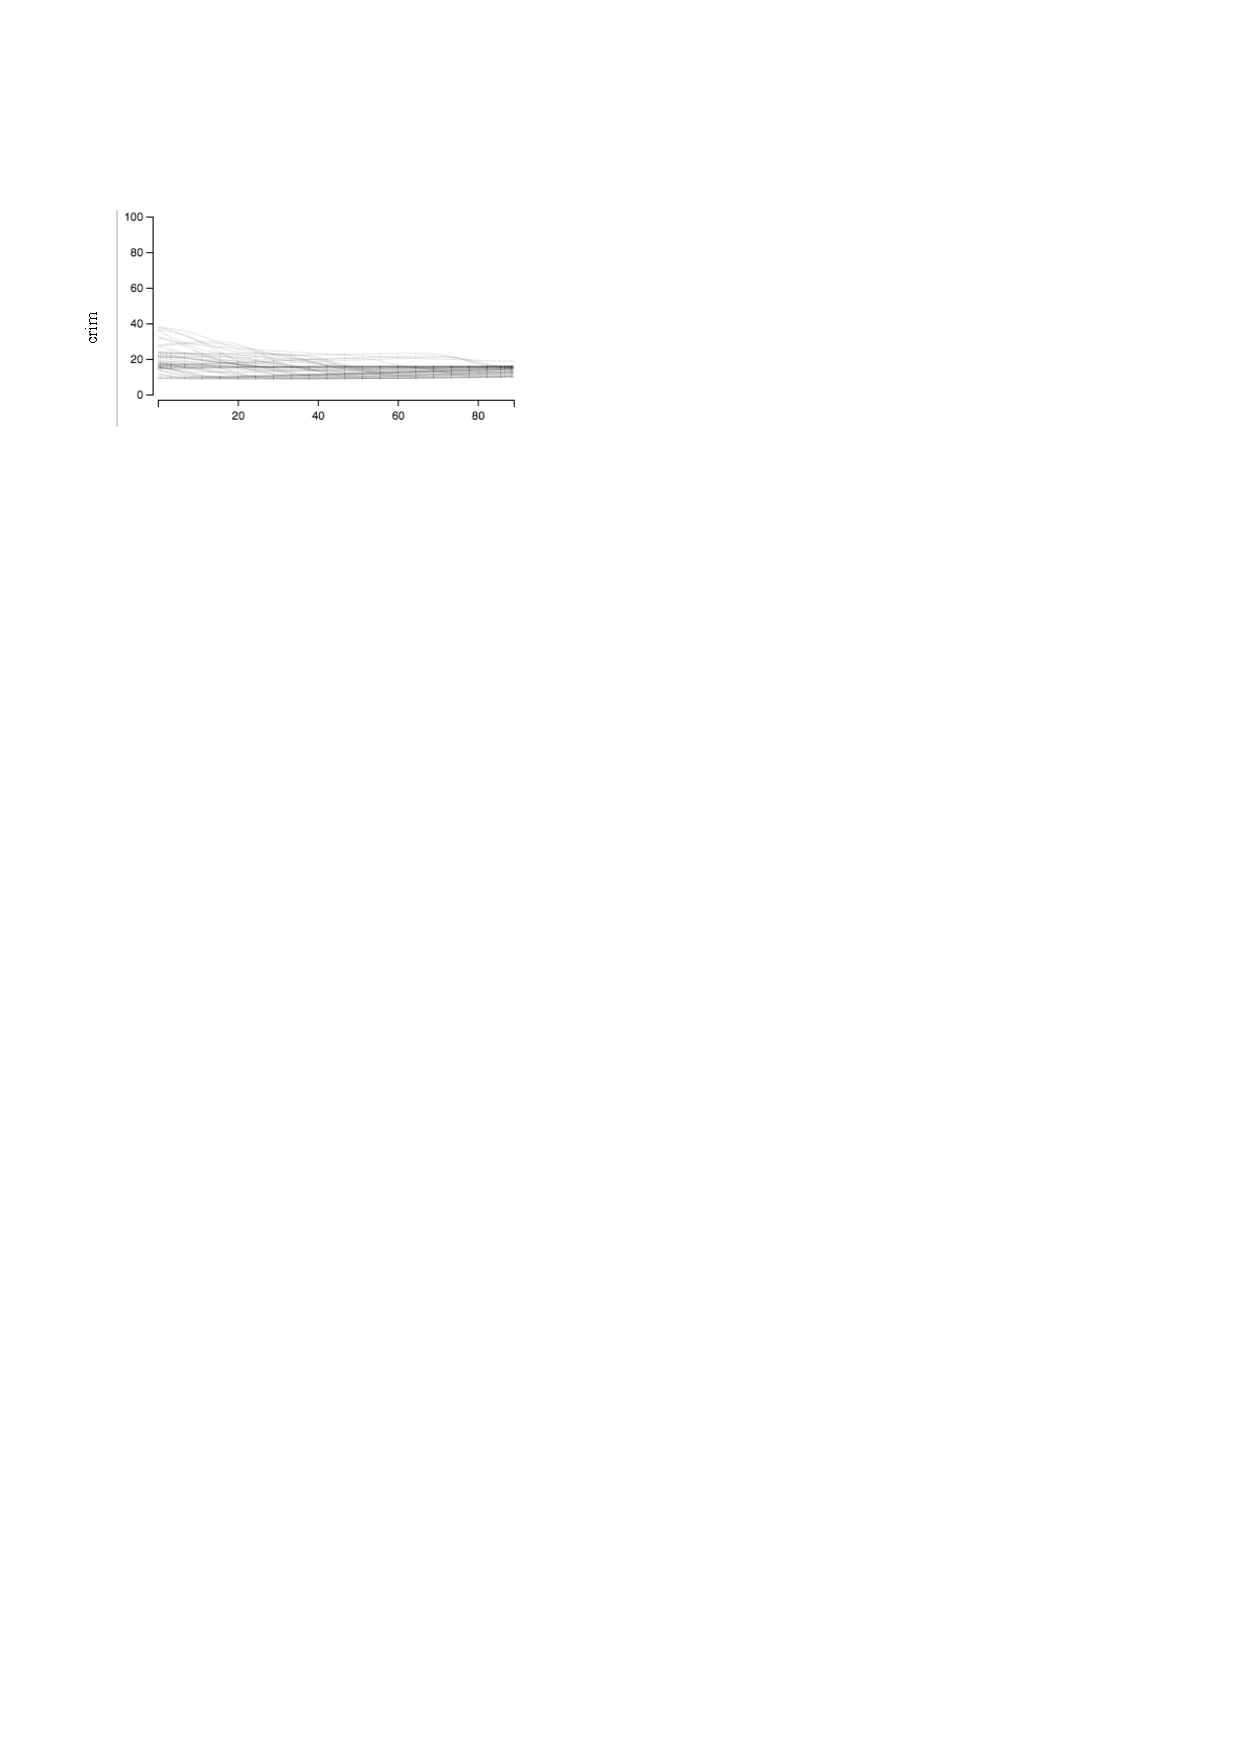
\includegraphics[width=\textwidth]{nn5x3_1.pdf}
    \end{subfigure}
    &
    \begin{subfigure}[b]{0.2\textwidth}
      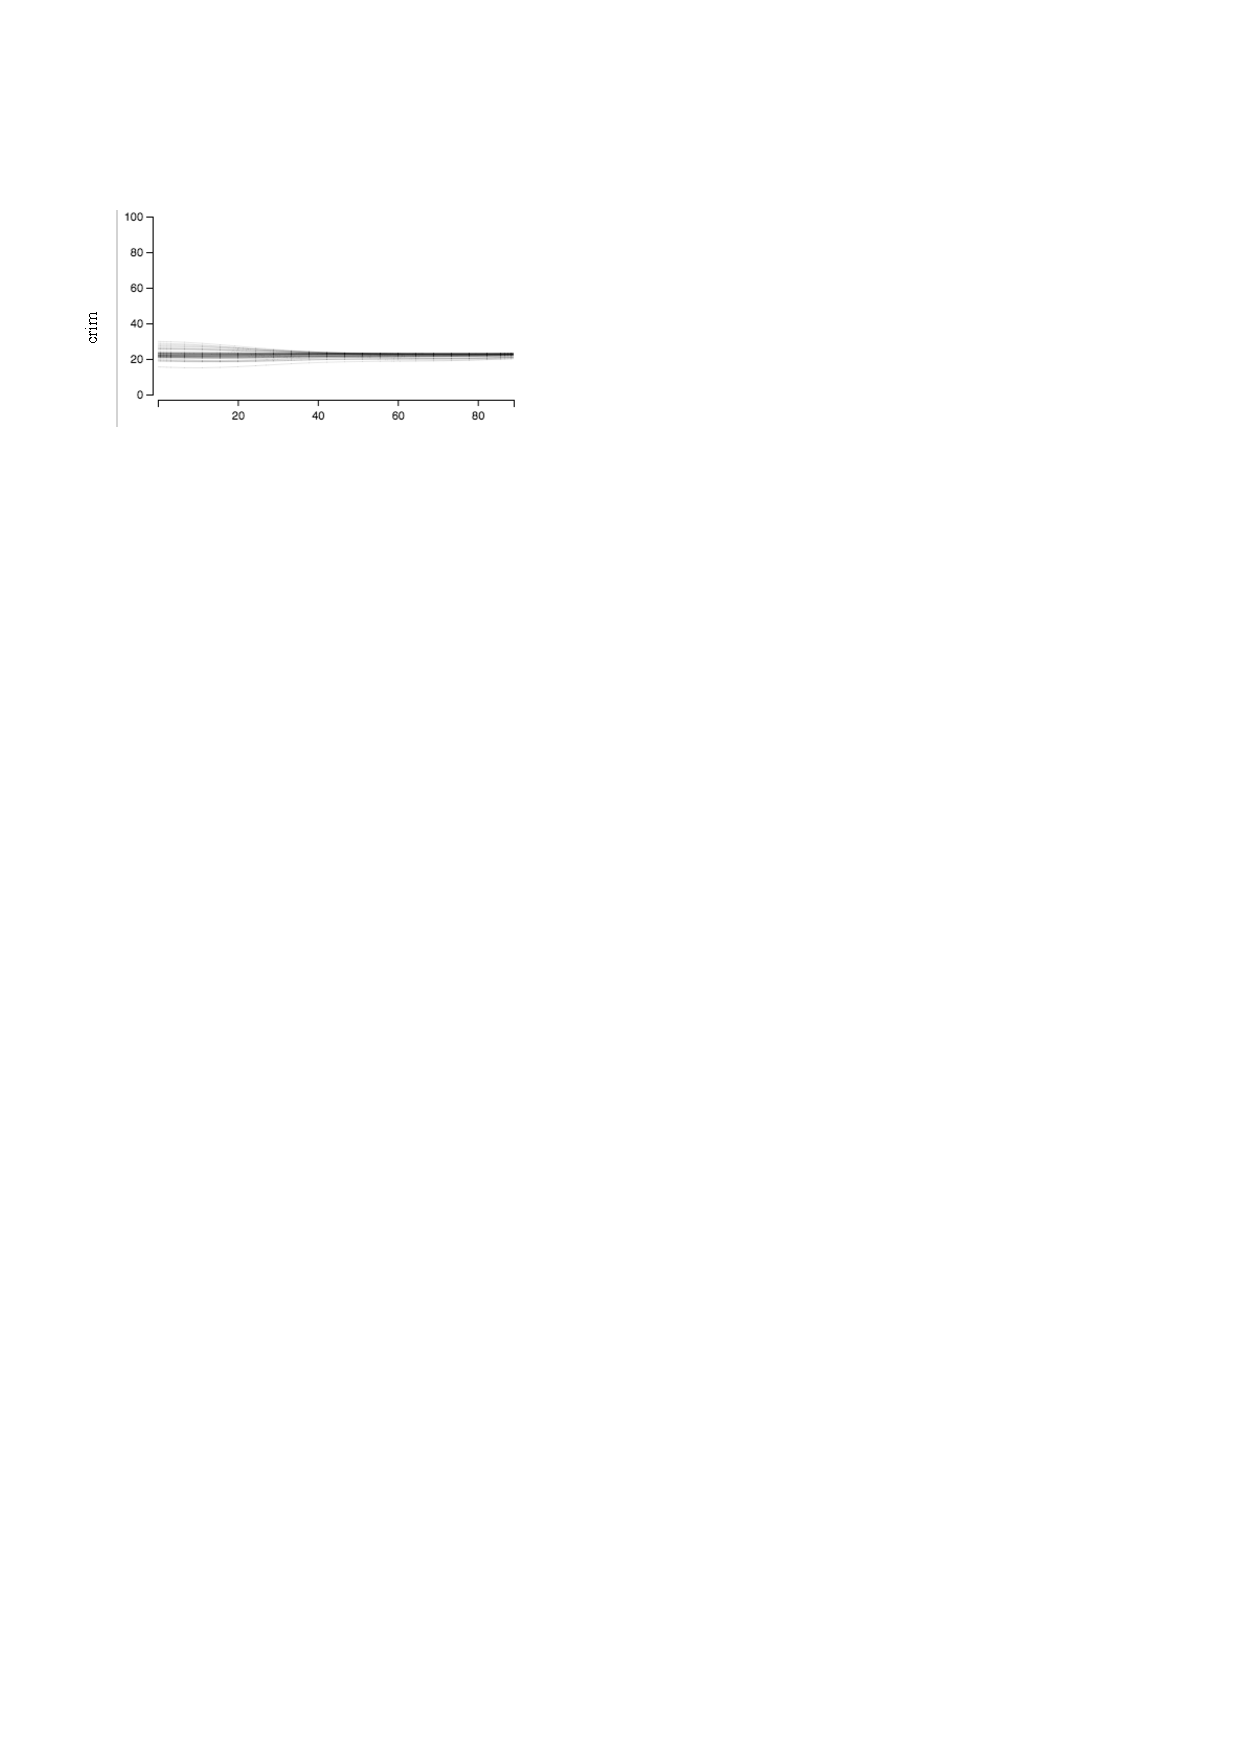
\includegraphics[width=\textwidth]{svmr_1.pdf}
    \end{subfigure}
    \\
    \hline \\
    Residential lots over 25,000 sq.ft. &
    \begin{subfigure}[b]{0.2\textwidth}
      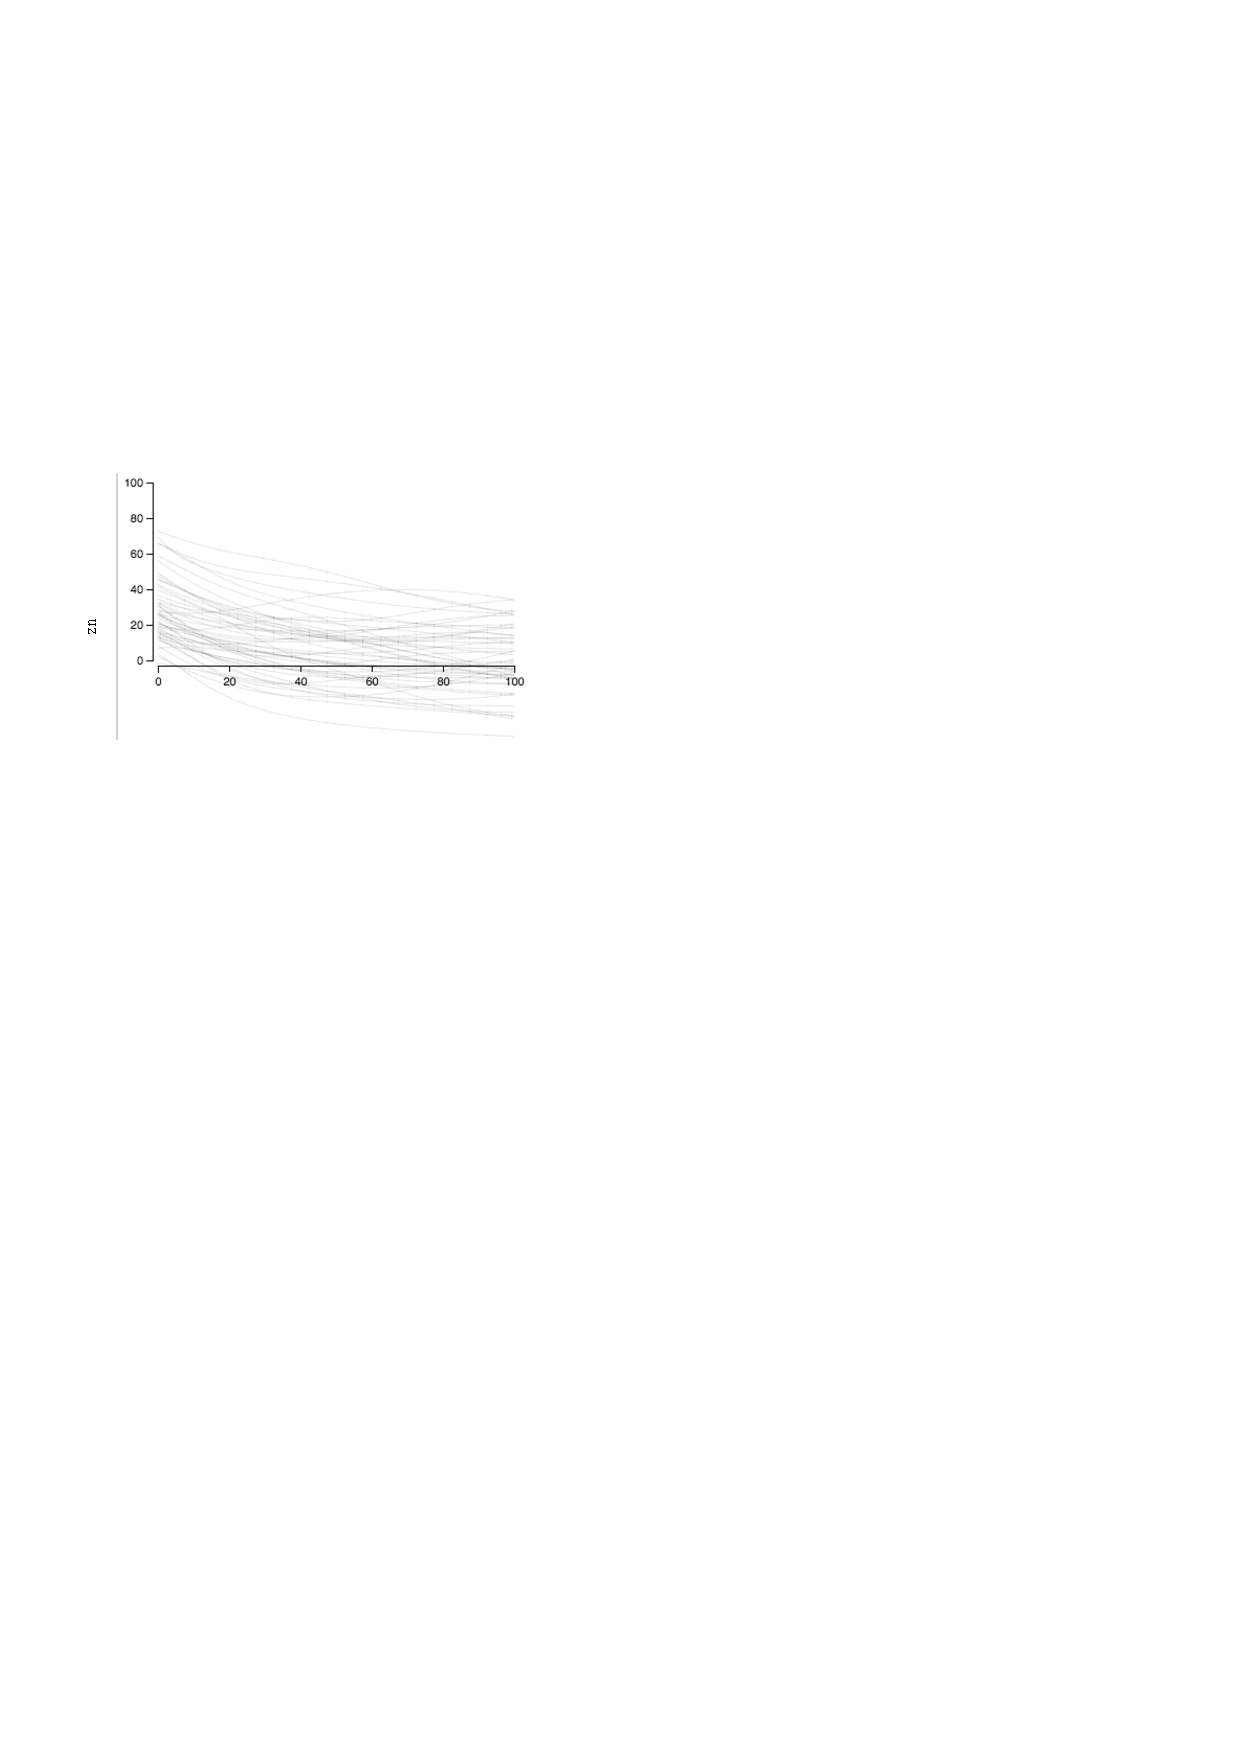
\includegraphics[width=\textwidth]{nn26_2.pdf}
    \end{subfigure}
    &
    \begin{subfigure}[b]{0.2\textwidth}
      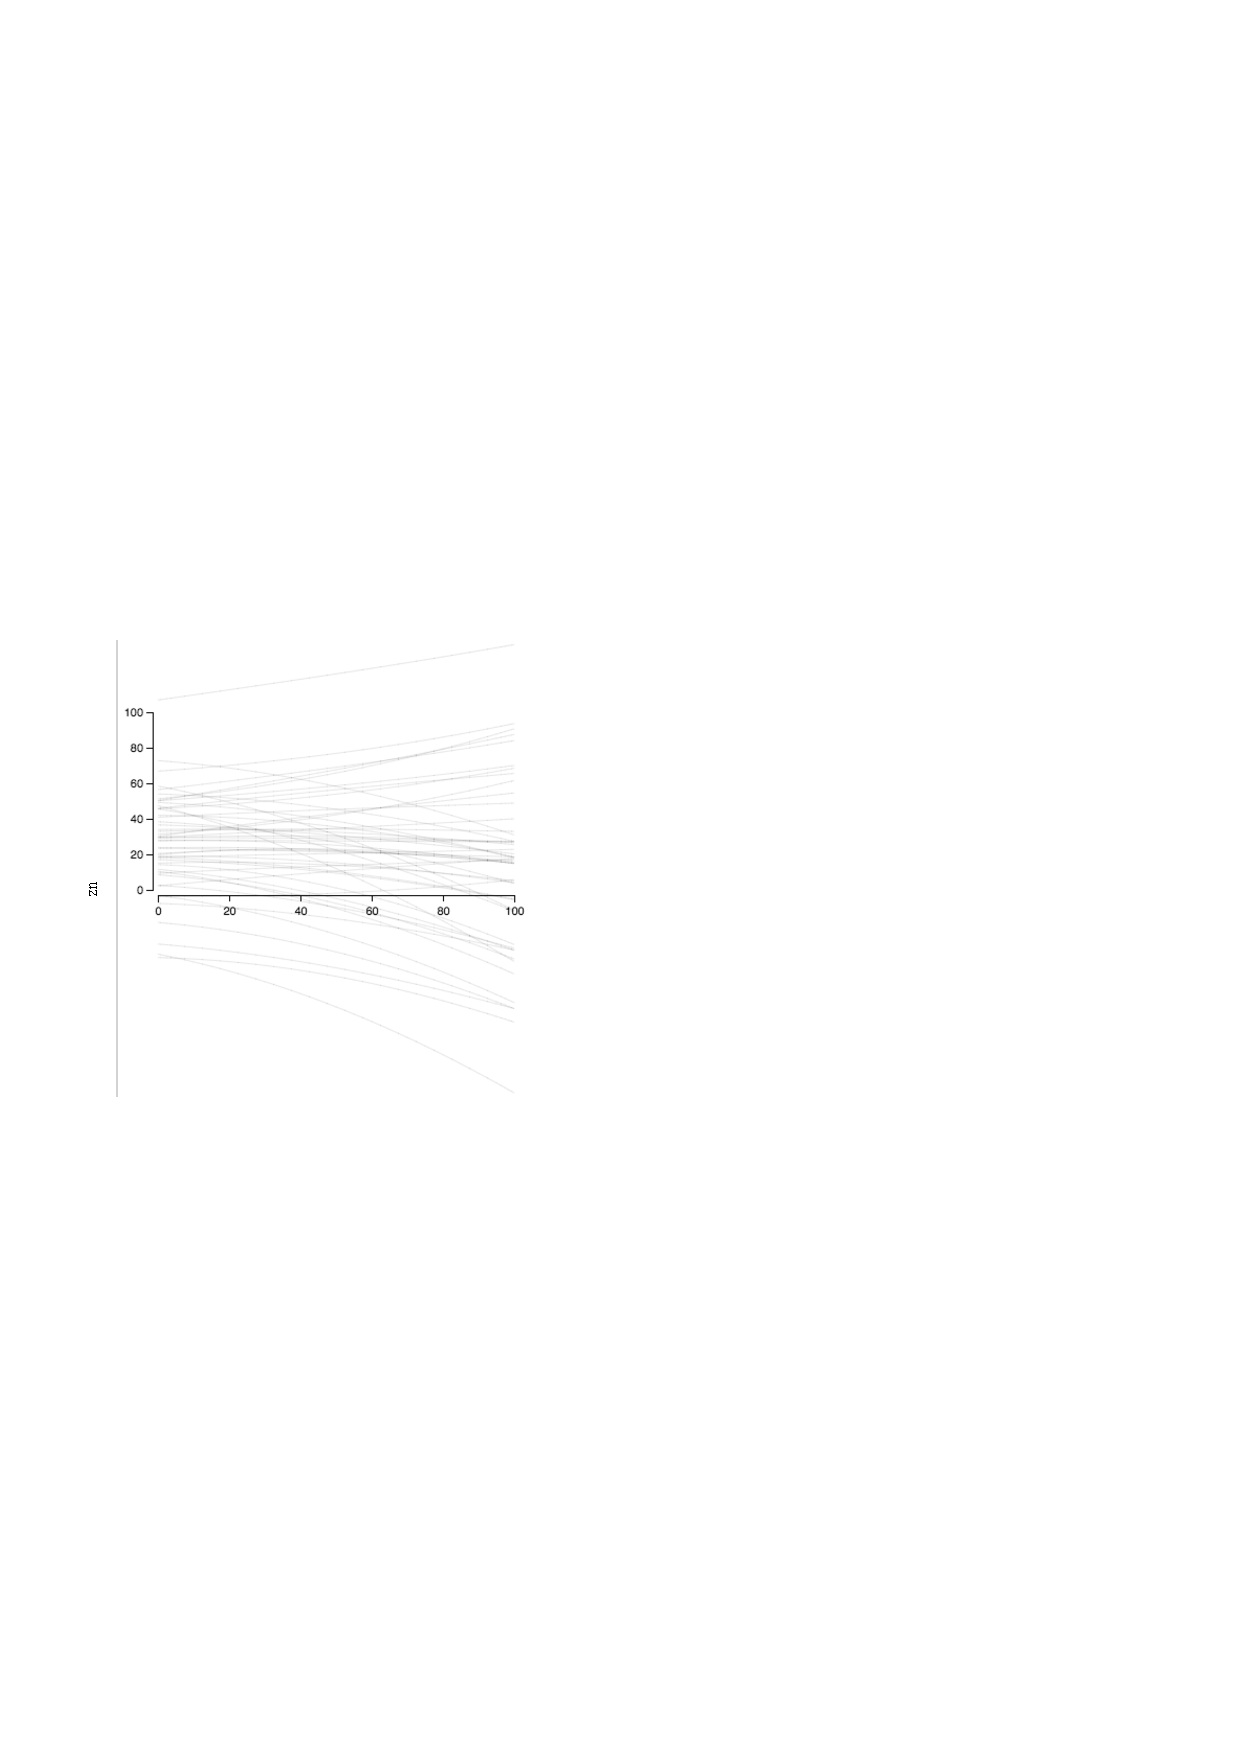
\includegraphics[width=\textwidth]{svmp_2.pdf}
    \end{subfigure}
    &
    \begin{subfigure}[b]{0.2\textwidth}
      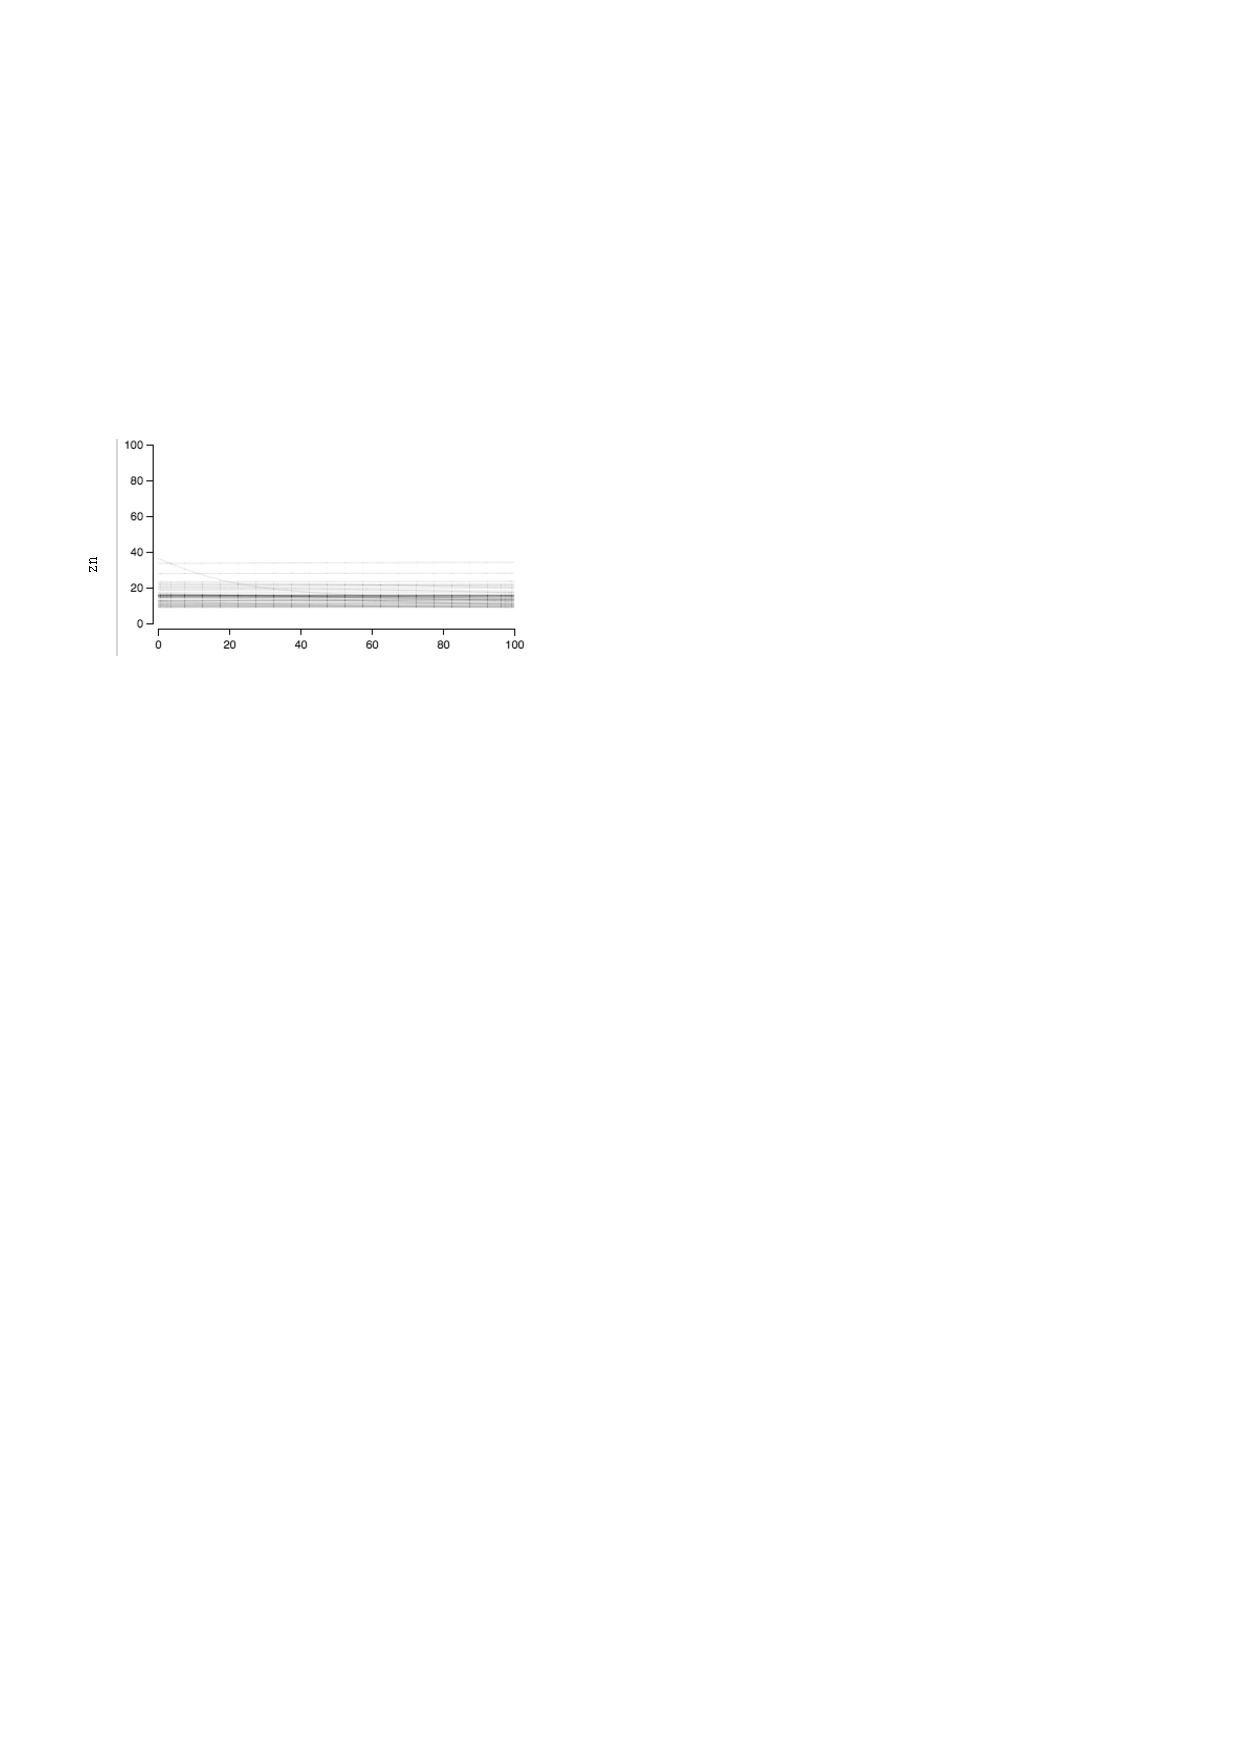
\includegraphics[width=\textwidth]{nn5x3_2.pdf}
    \end{subfigure}
    &
    \begin{subfigure}[b]{0.2\textwidth}
      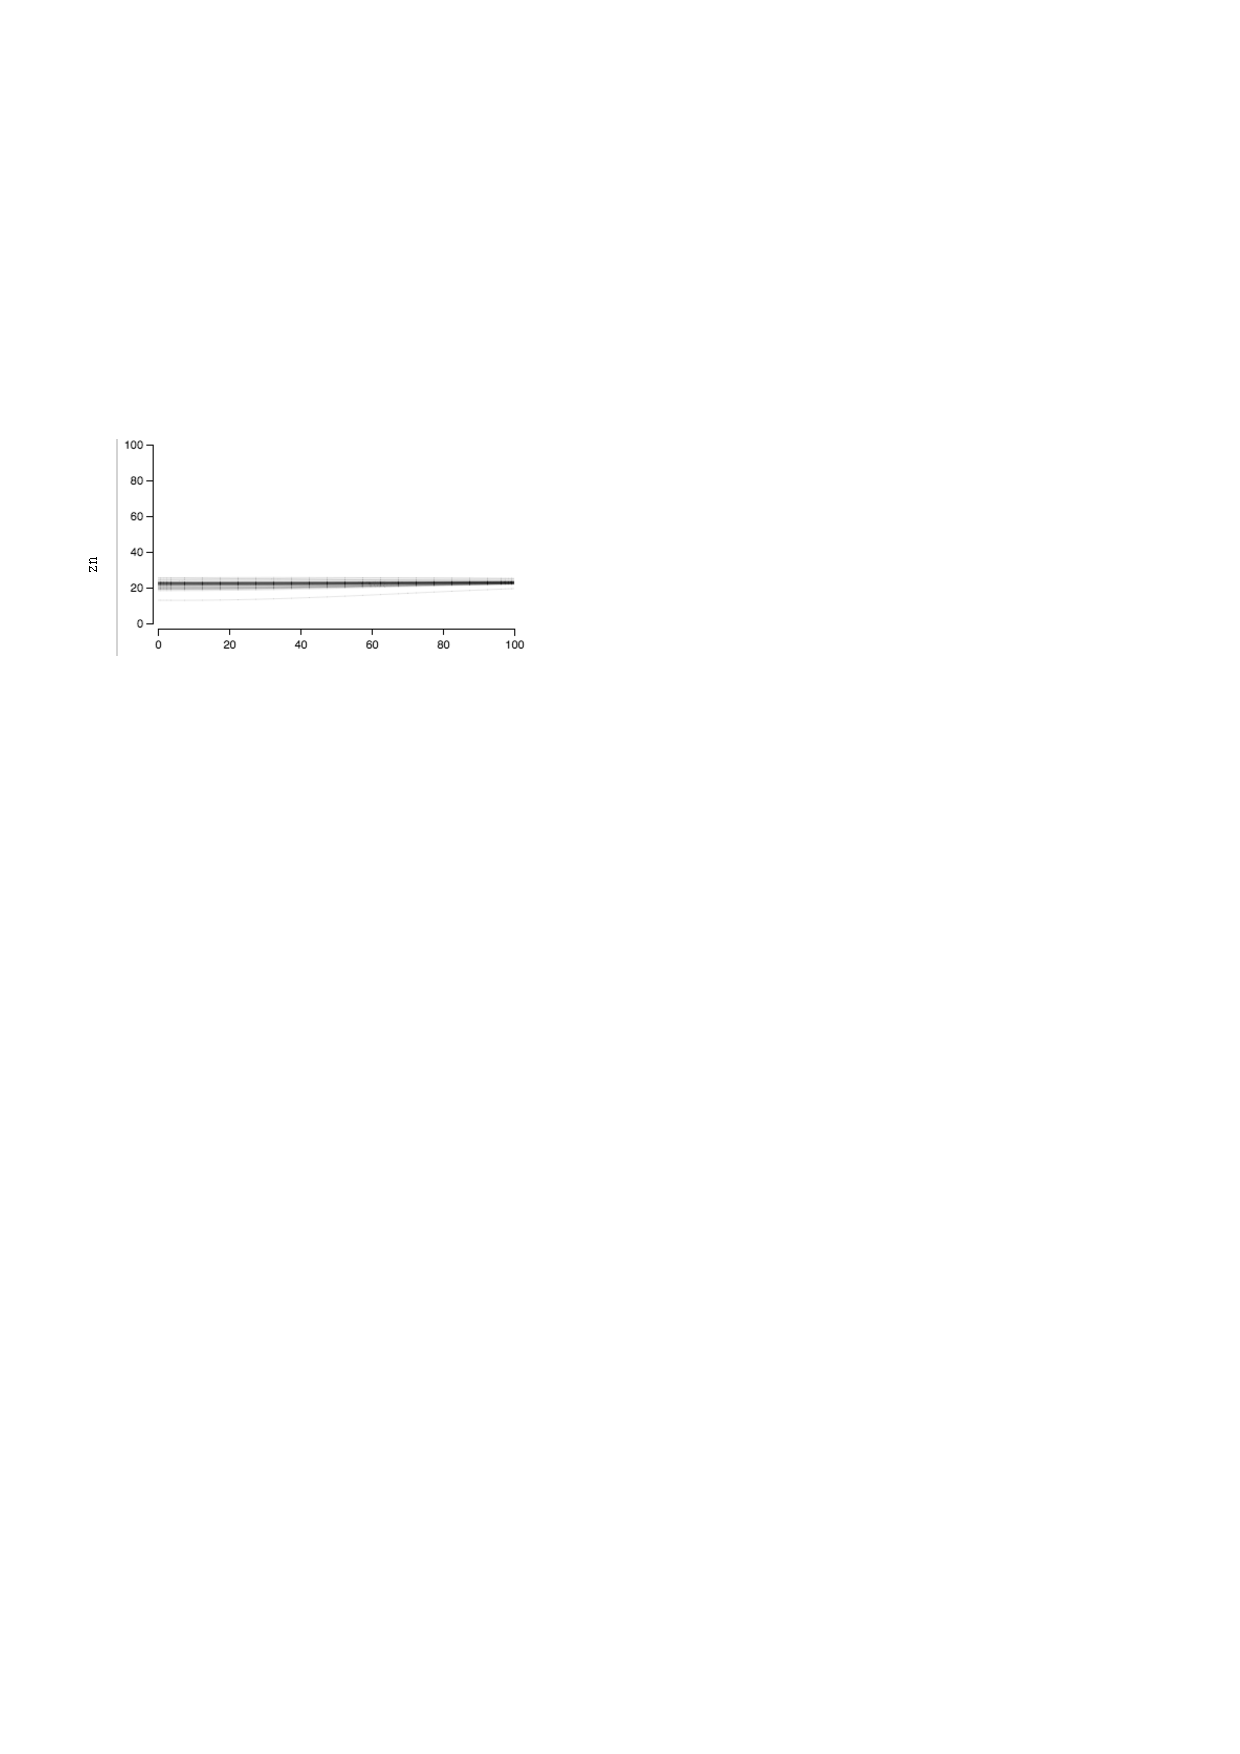
\includegraphics[width=\textwidth]{svmr_2.pdf}
    \end{subfigure}
    \\
    \hline \\
    Non-retail business acres &
    \begin{subfigure}[b]{0.2\textwidth}
      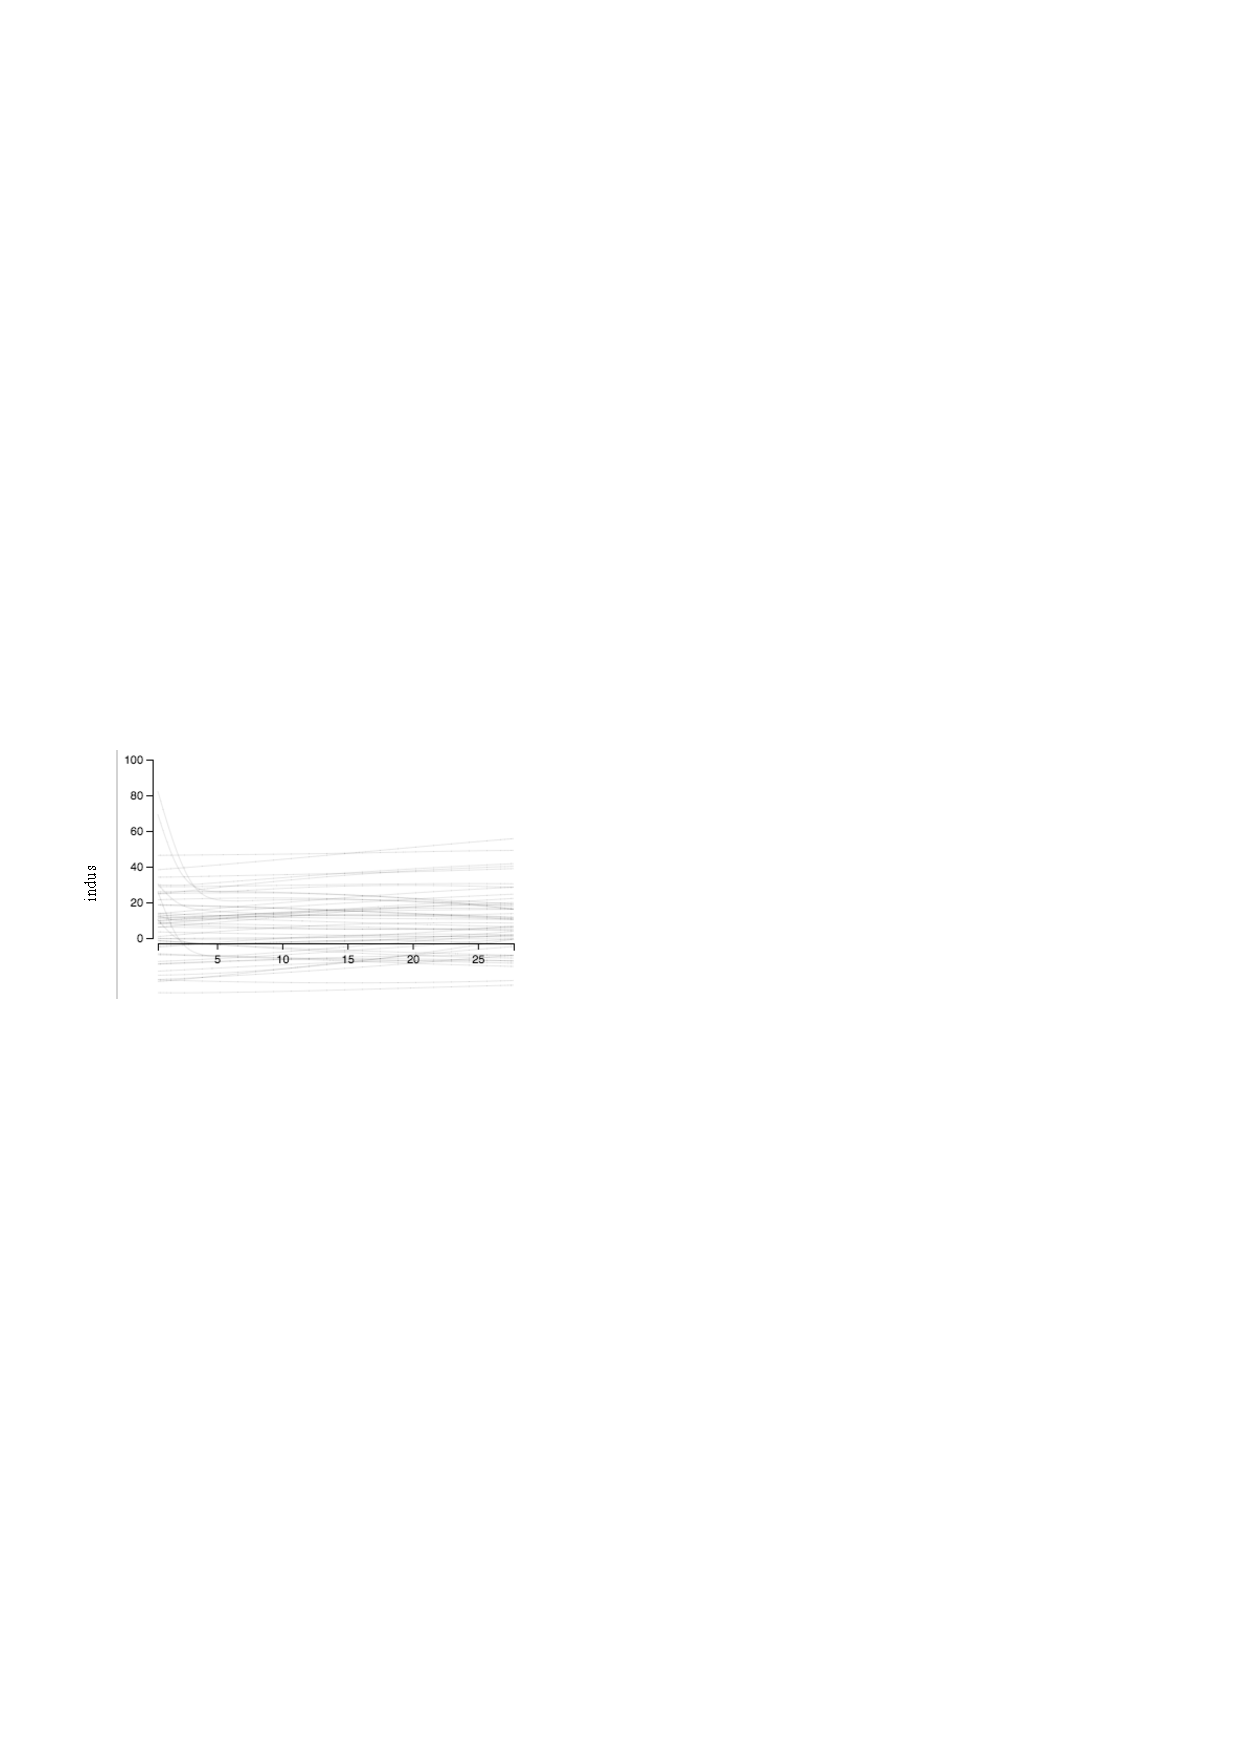
\includegraphics[width=\textwidth]{nn26_3.pdf}
    \end{subfigure}
    &
    \begin{subfigure}[b]{0.2\textwidth}
      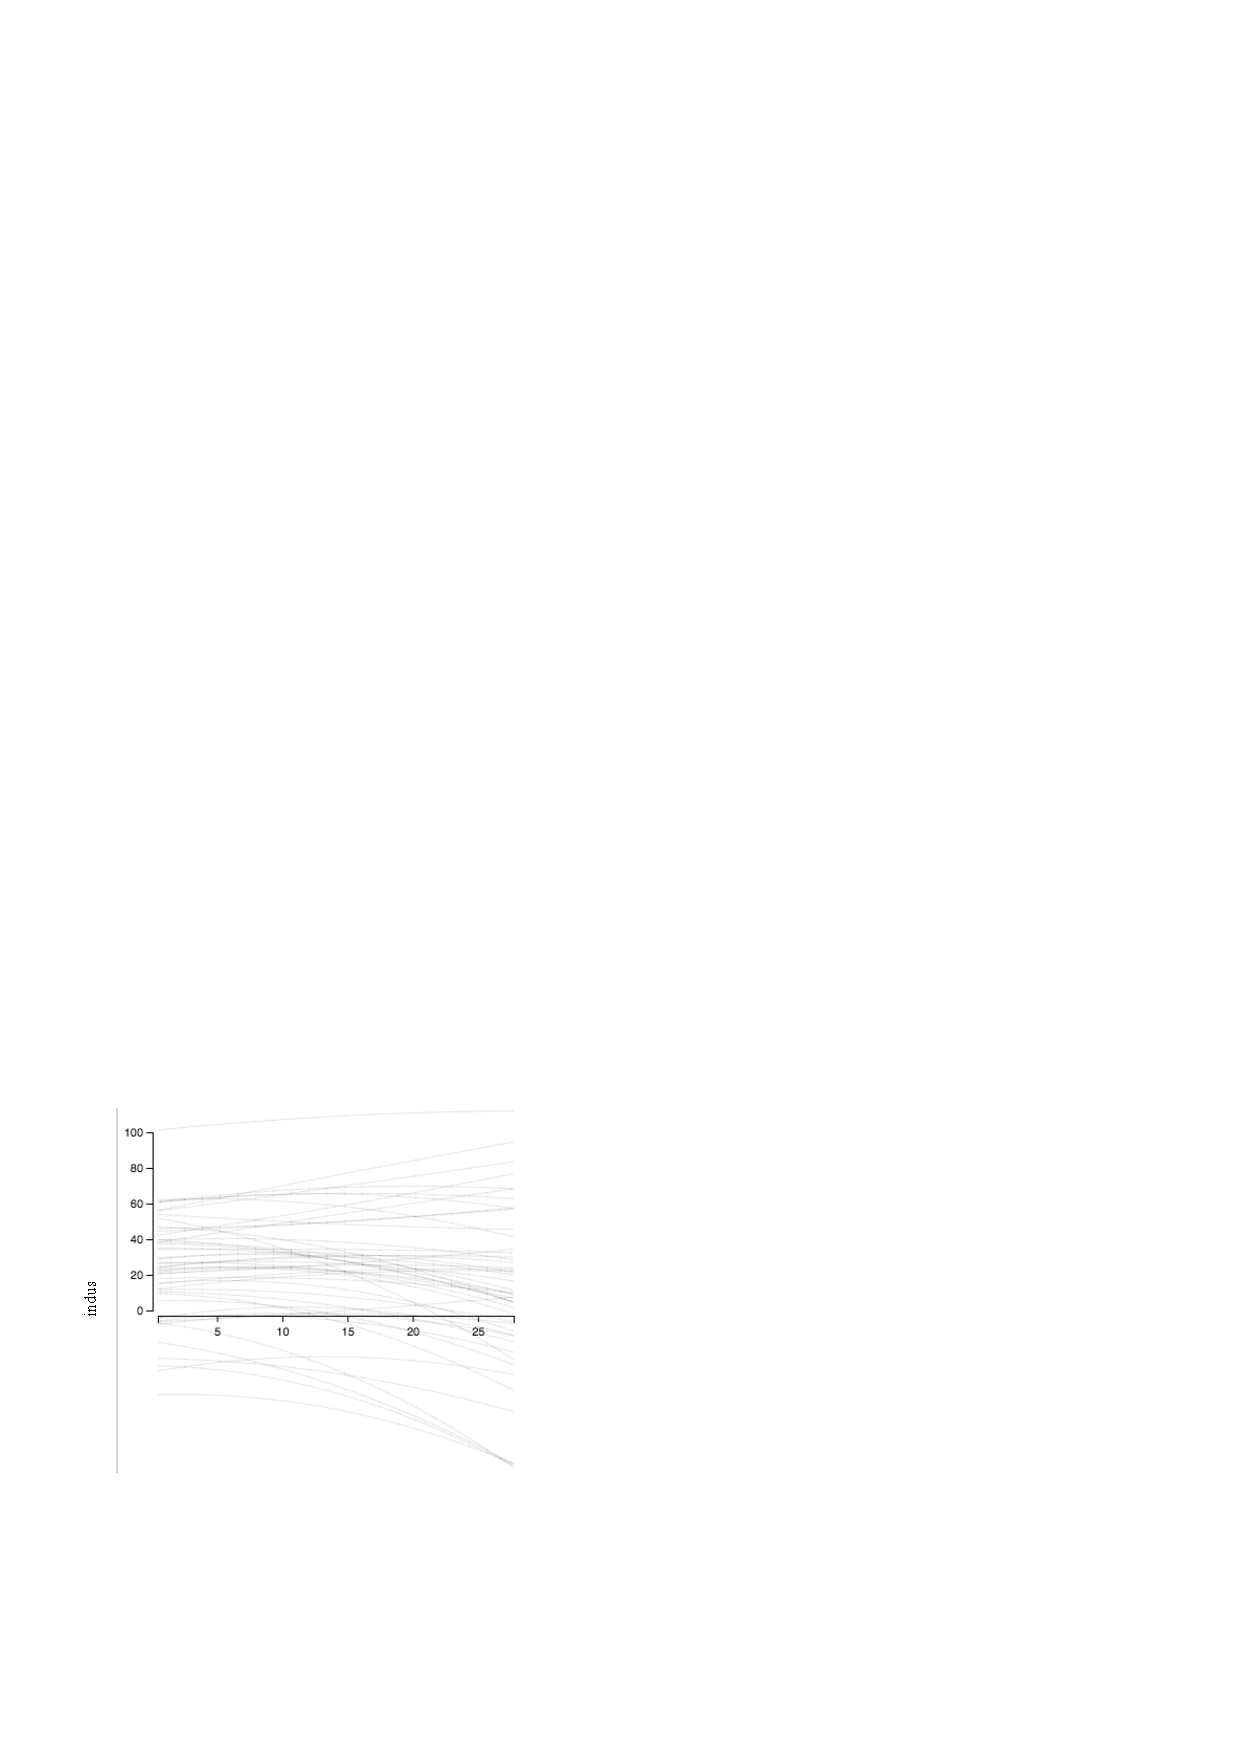
\includegraphics[width=\textwidth]{svmp_3.pdf}
    \end{subfigure}
    &
    \begin{subfigure}[b]{0.2\textwidth}
      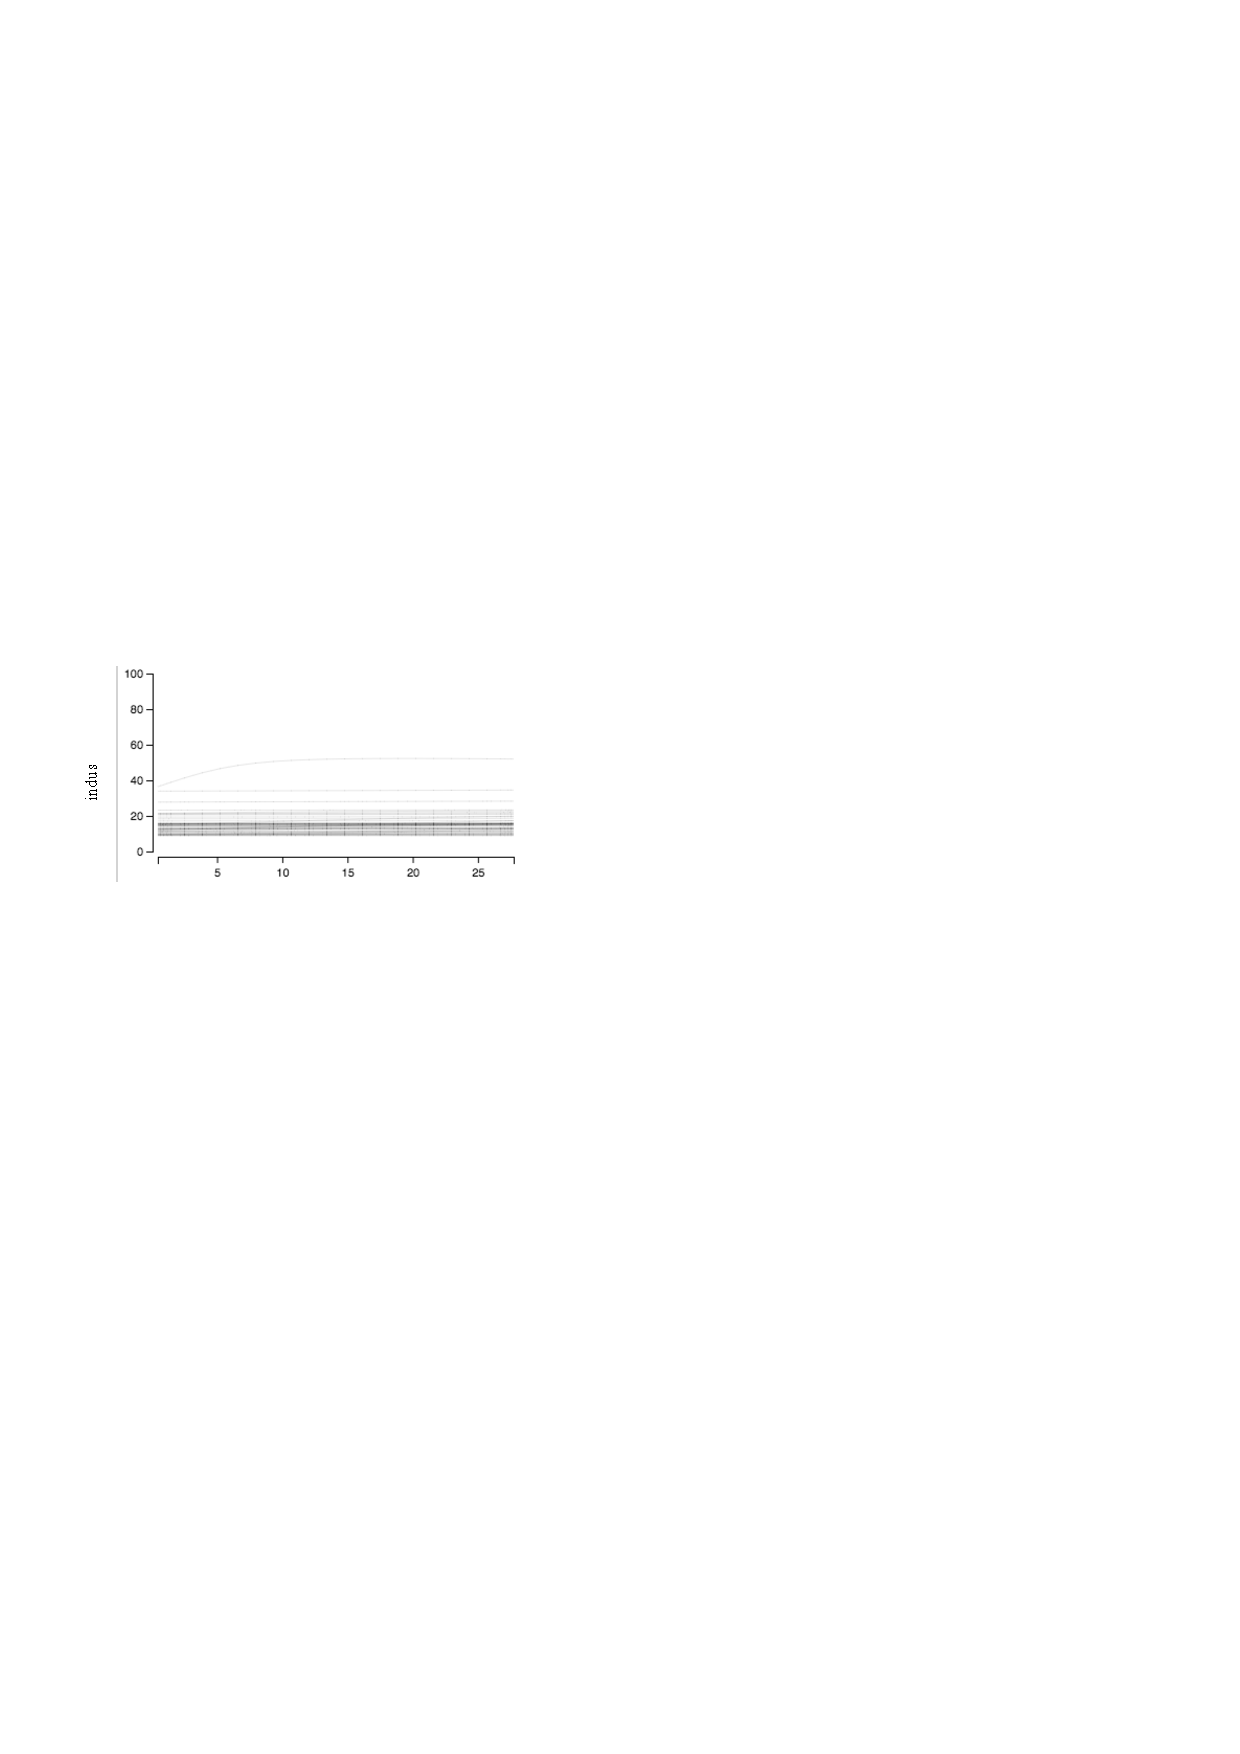
\includegraphics[width=\textwidth]{nn5x3_3.pdf}
    \end{subfigure}
    &
    \begin{subfigure}[b]{0.2\textwidth}
      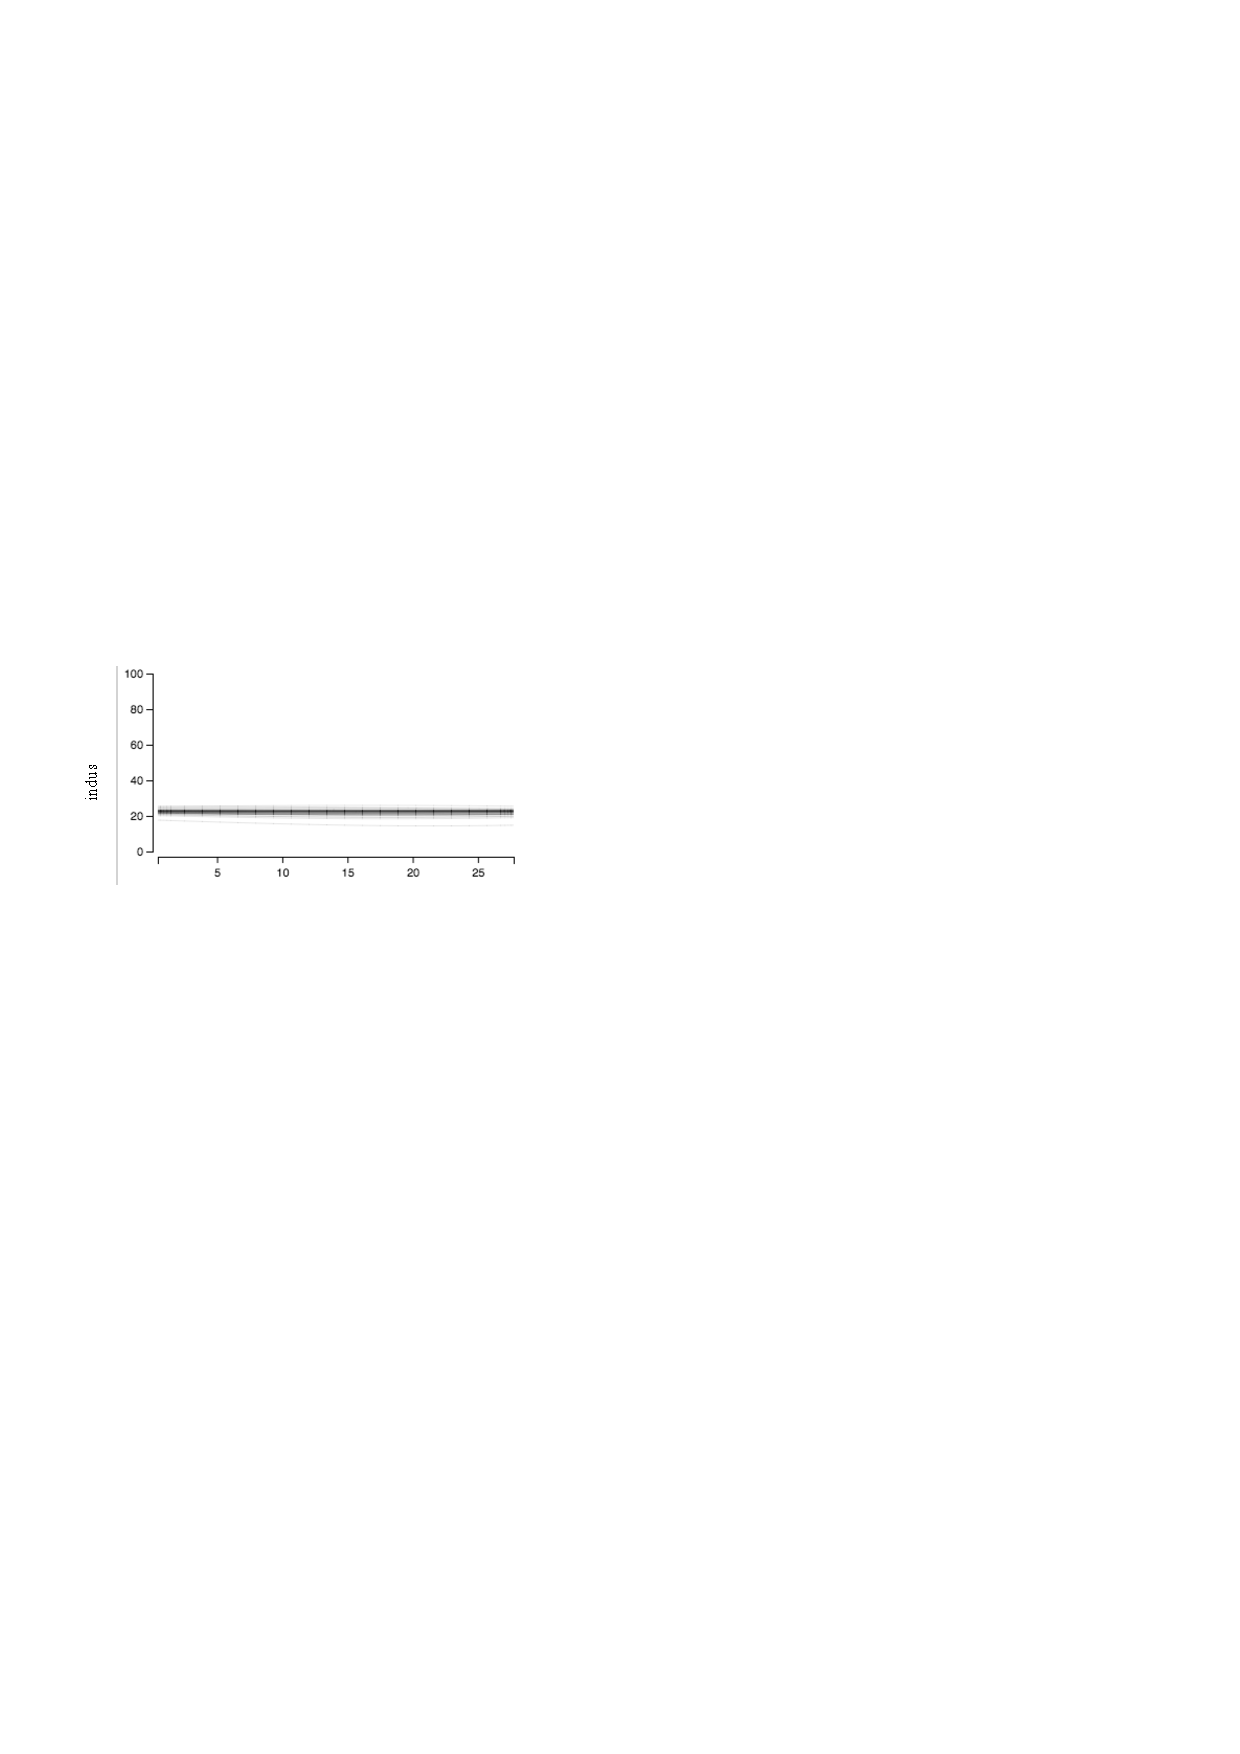
\includegraphics[width=\textwidth]{svmr_3.pdf}
    \end{subfigure}
    \\
    \hline \\
    1 if tract bounds river &
    \begin{subfigure}[b]{0.2\textwidth}
      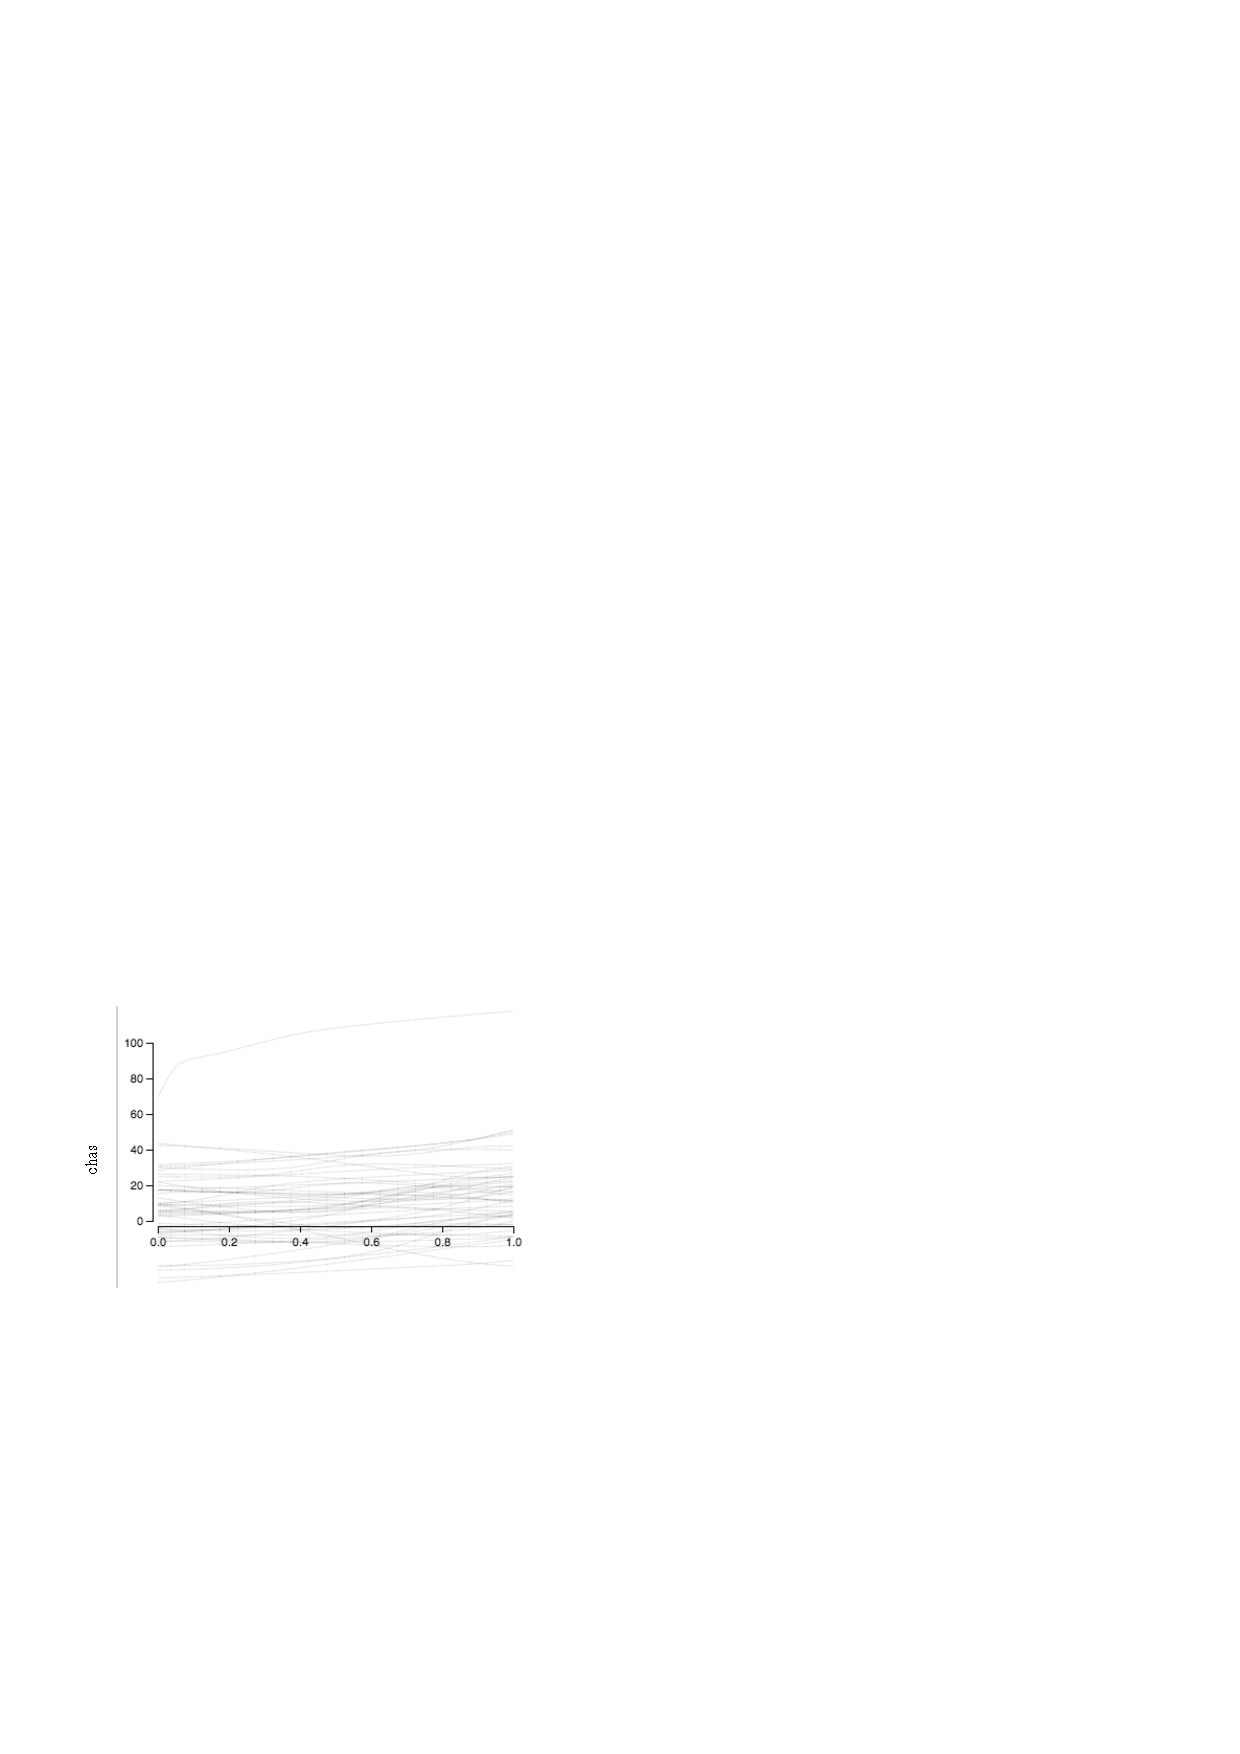
\includegraphics[width=\textwidth]{nn26_4.pdf}
    \end{subfigure}
    &
    \begin{subfigure}[b]{0.2\textwidth}
      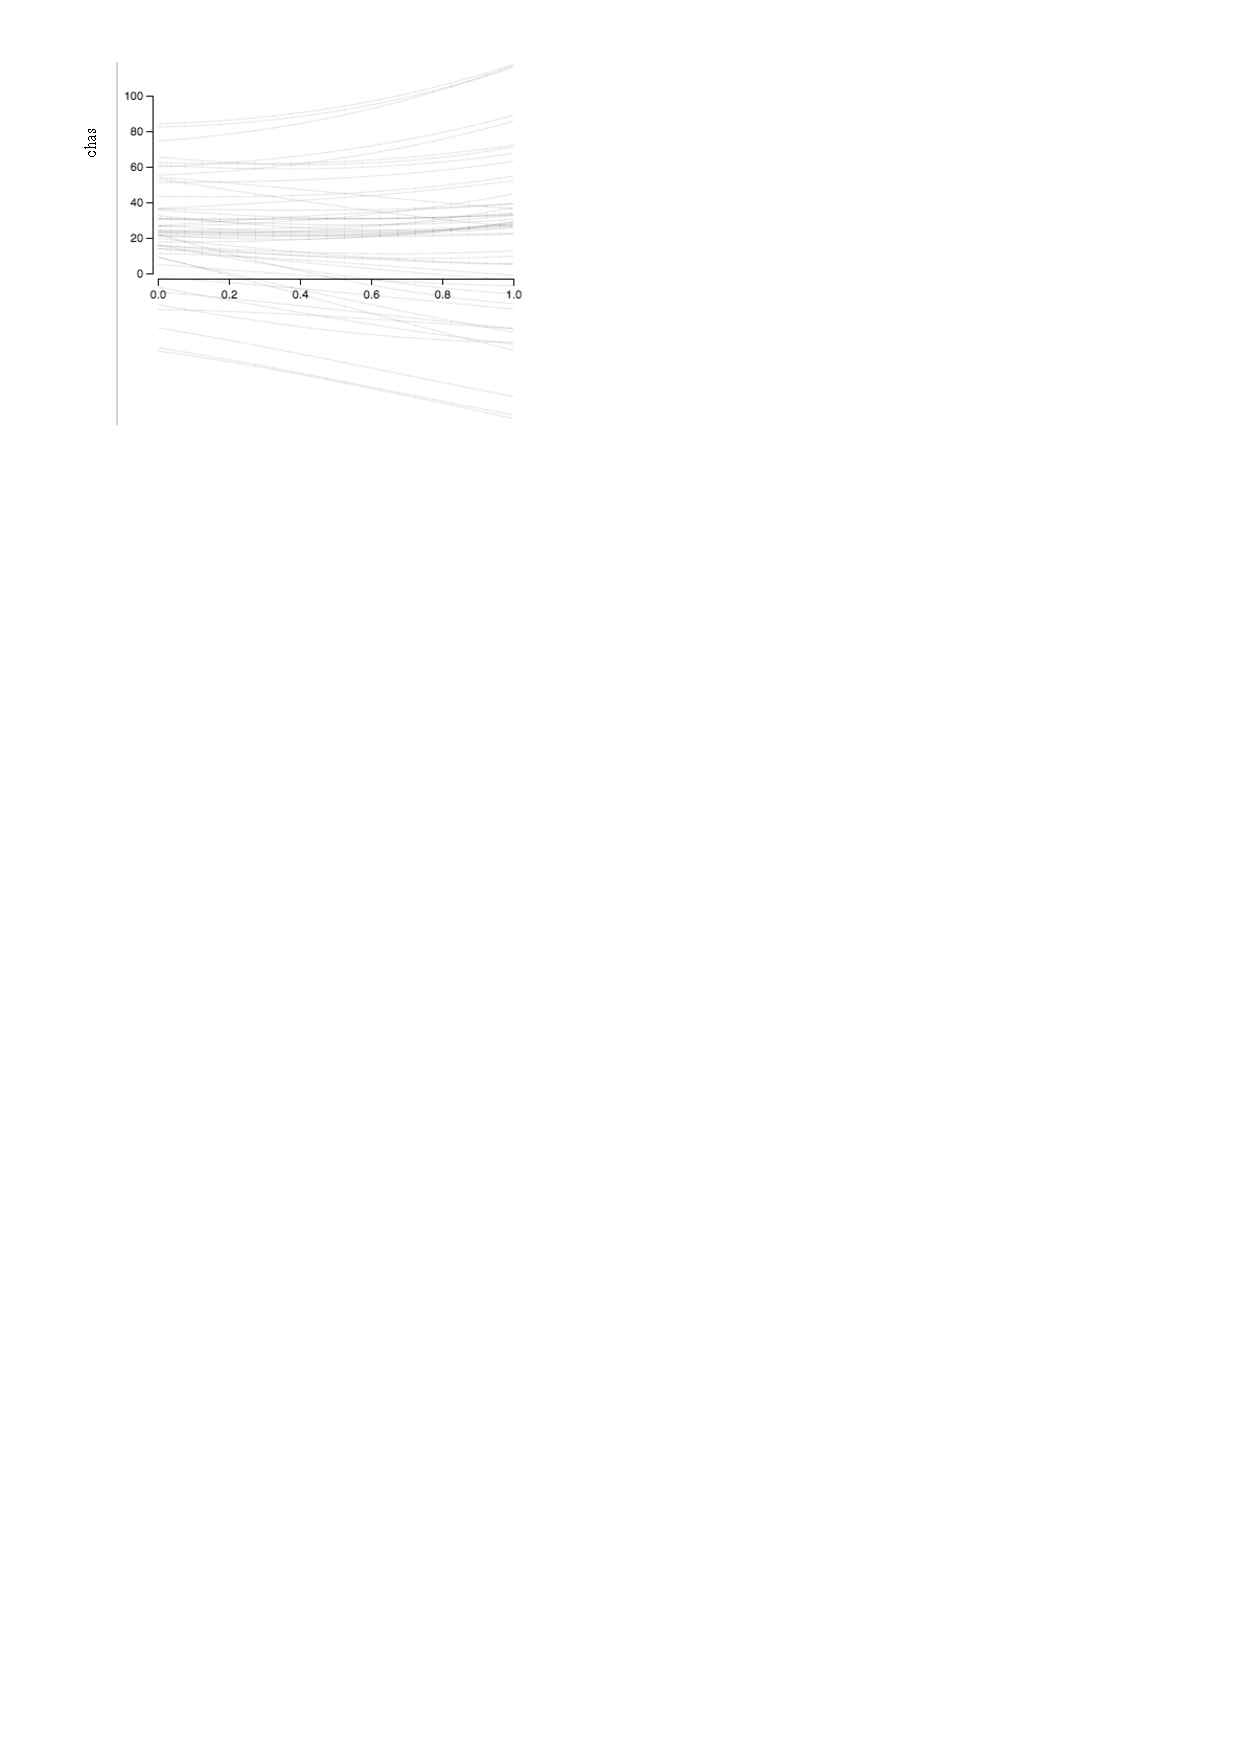
\includegraphics[width=\textwidth]{svmp_4.pdf}
    \end{subfigure}
    &
    \begin{subfigure}[b]{0.2\textwidth}
      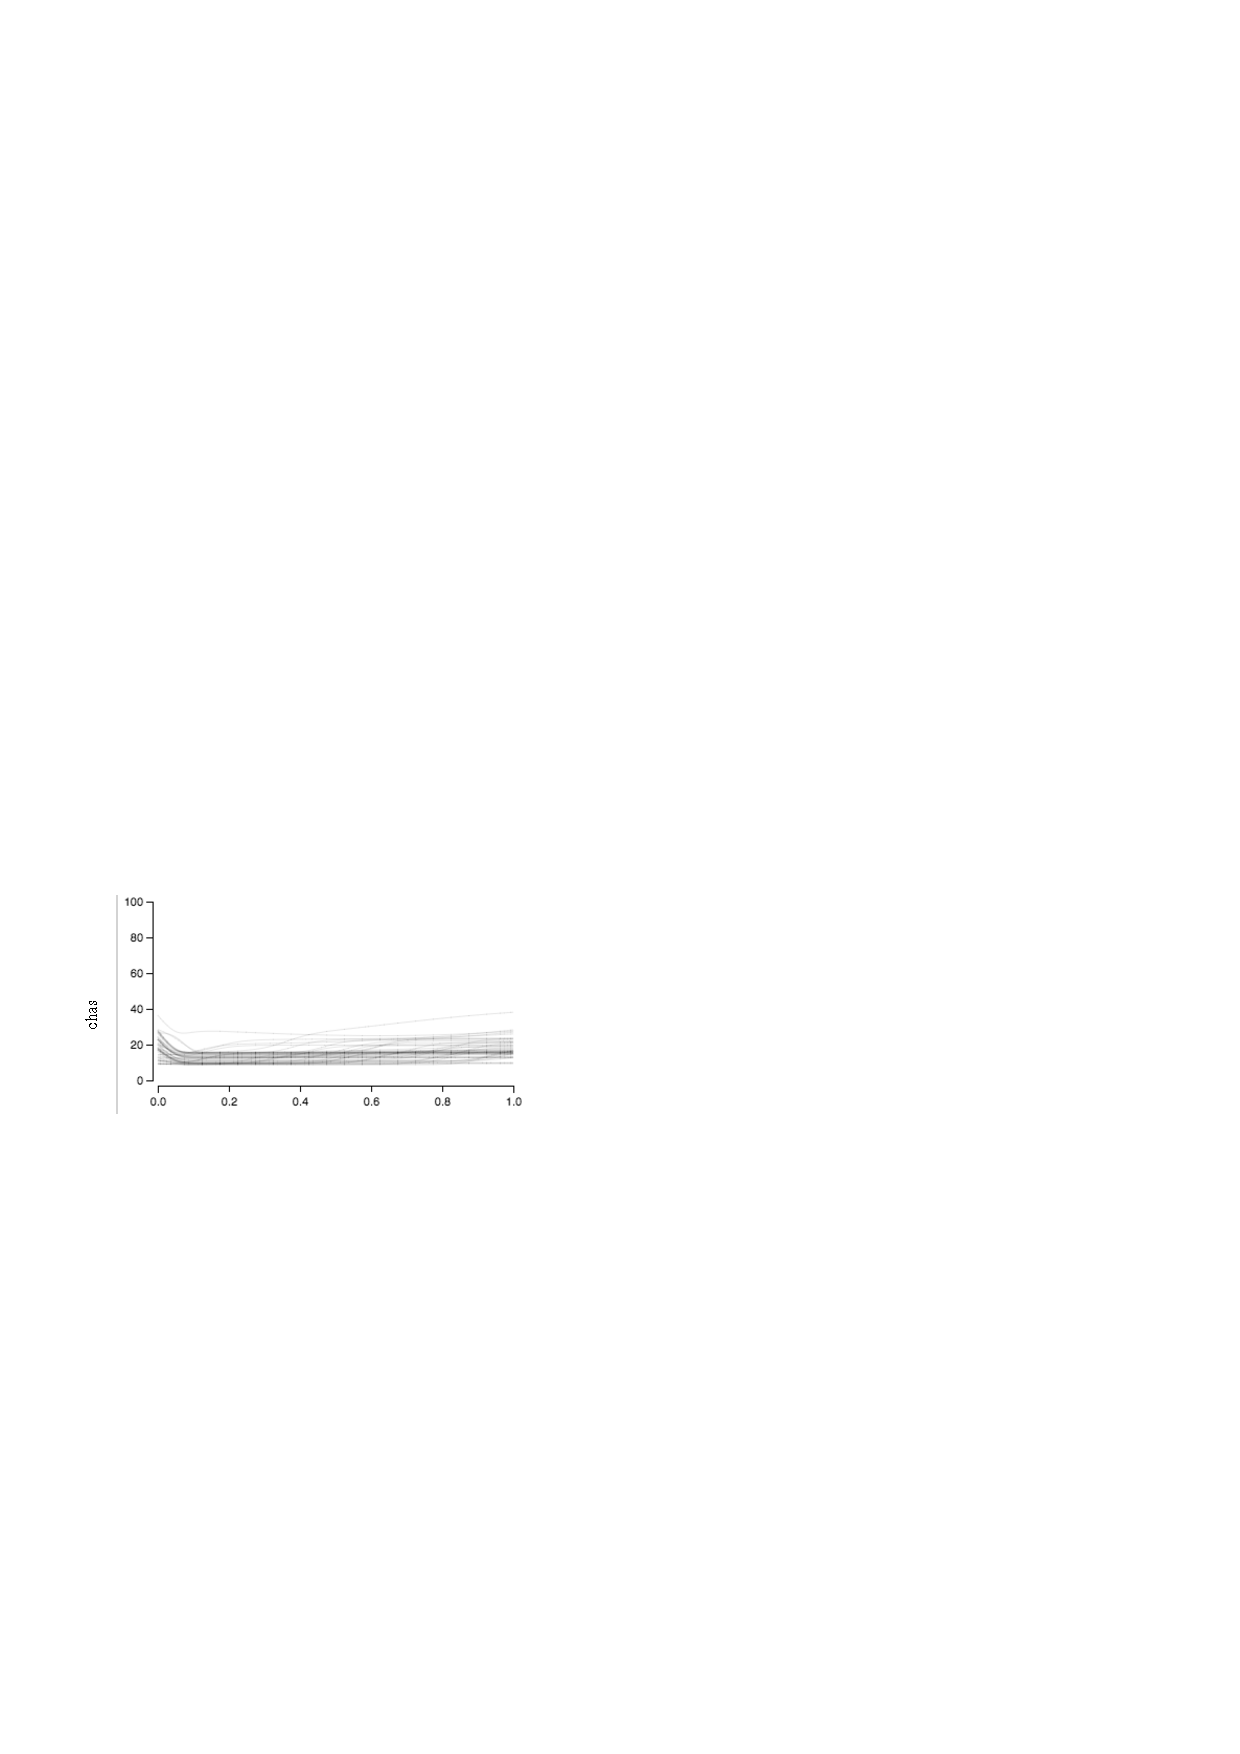
\includegraphics[width=\textwidth]{nn5x3_4.pdf}
    \end{subfigure}
    &
    \begin{subfigure}[b]{0.2\textwidth}
      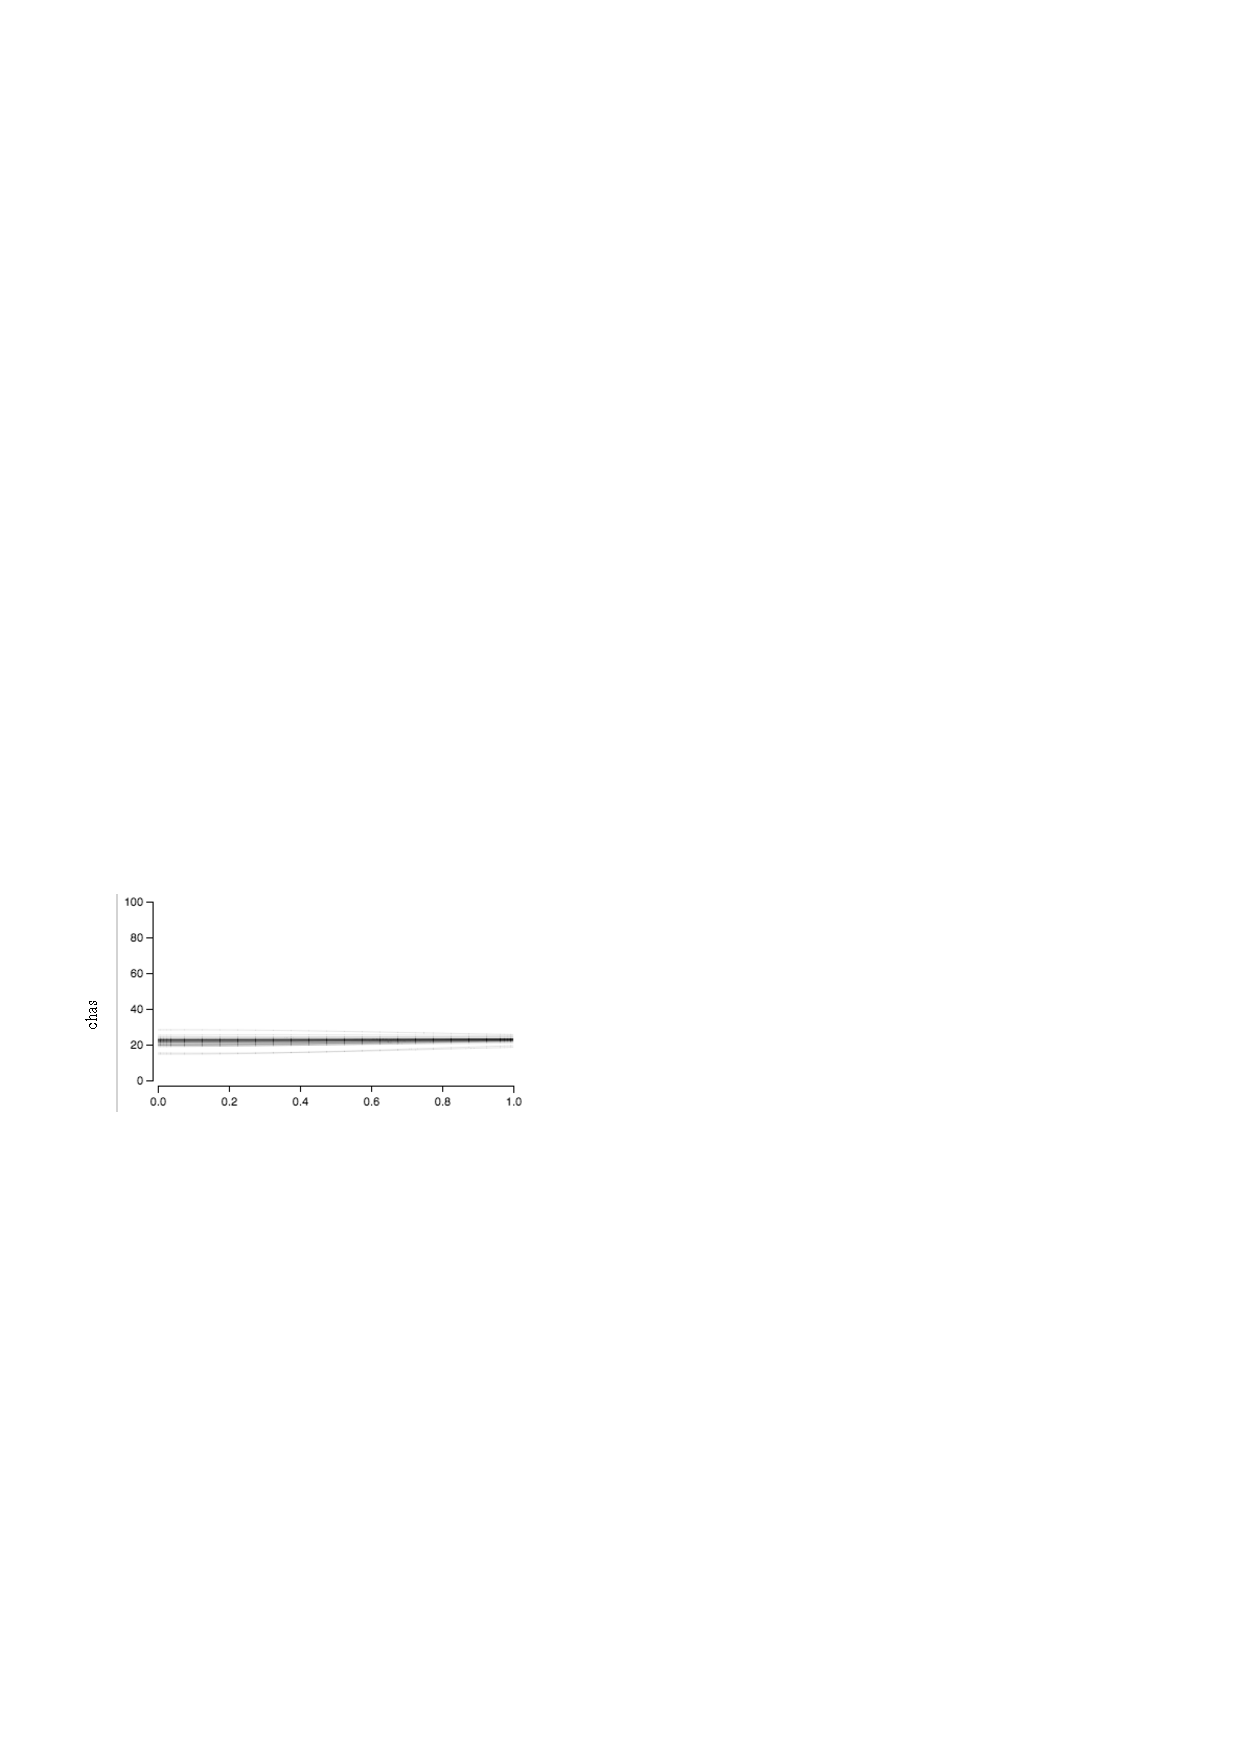
\includegraphics[width=\textwidth]{svmr_4.pdf}
    \end{subfigure}
    \\
    \hline \\
    Nitric oxide concentration &
    \begin{subfigure}[b]{0.2\textwidth}
      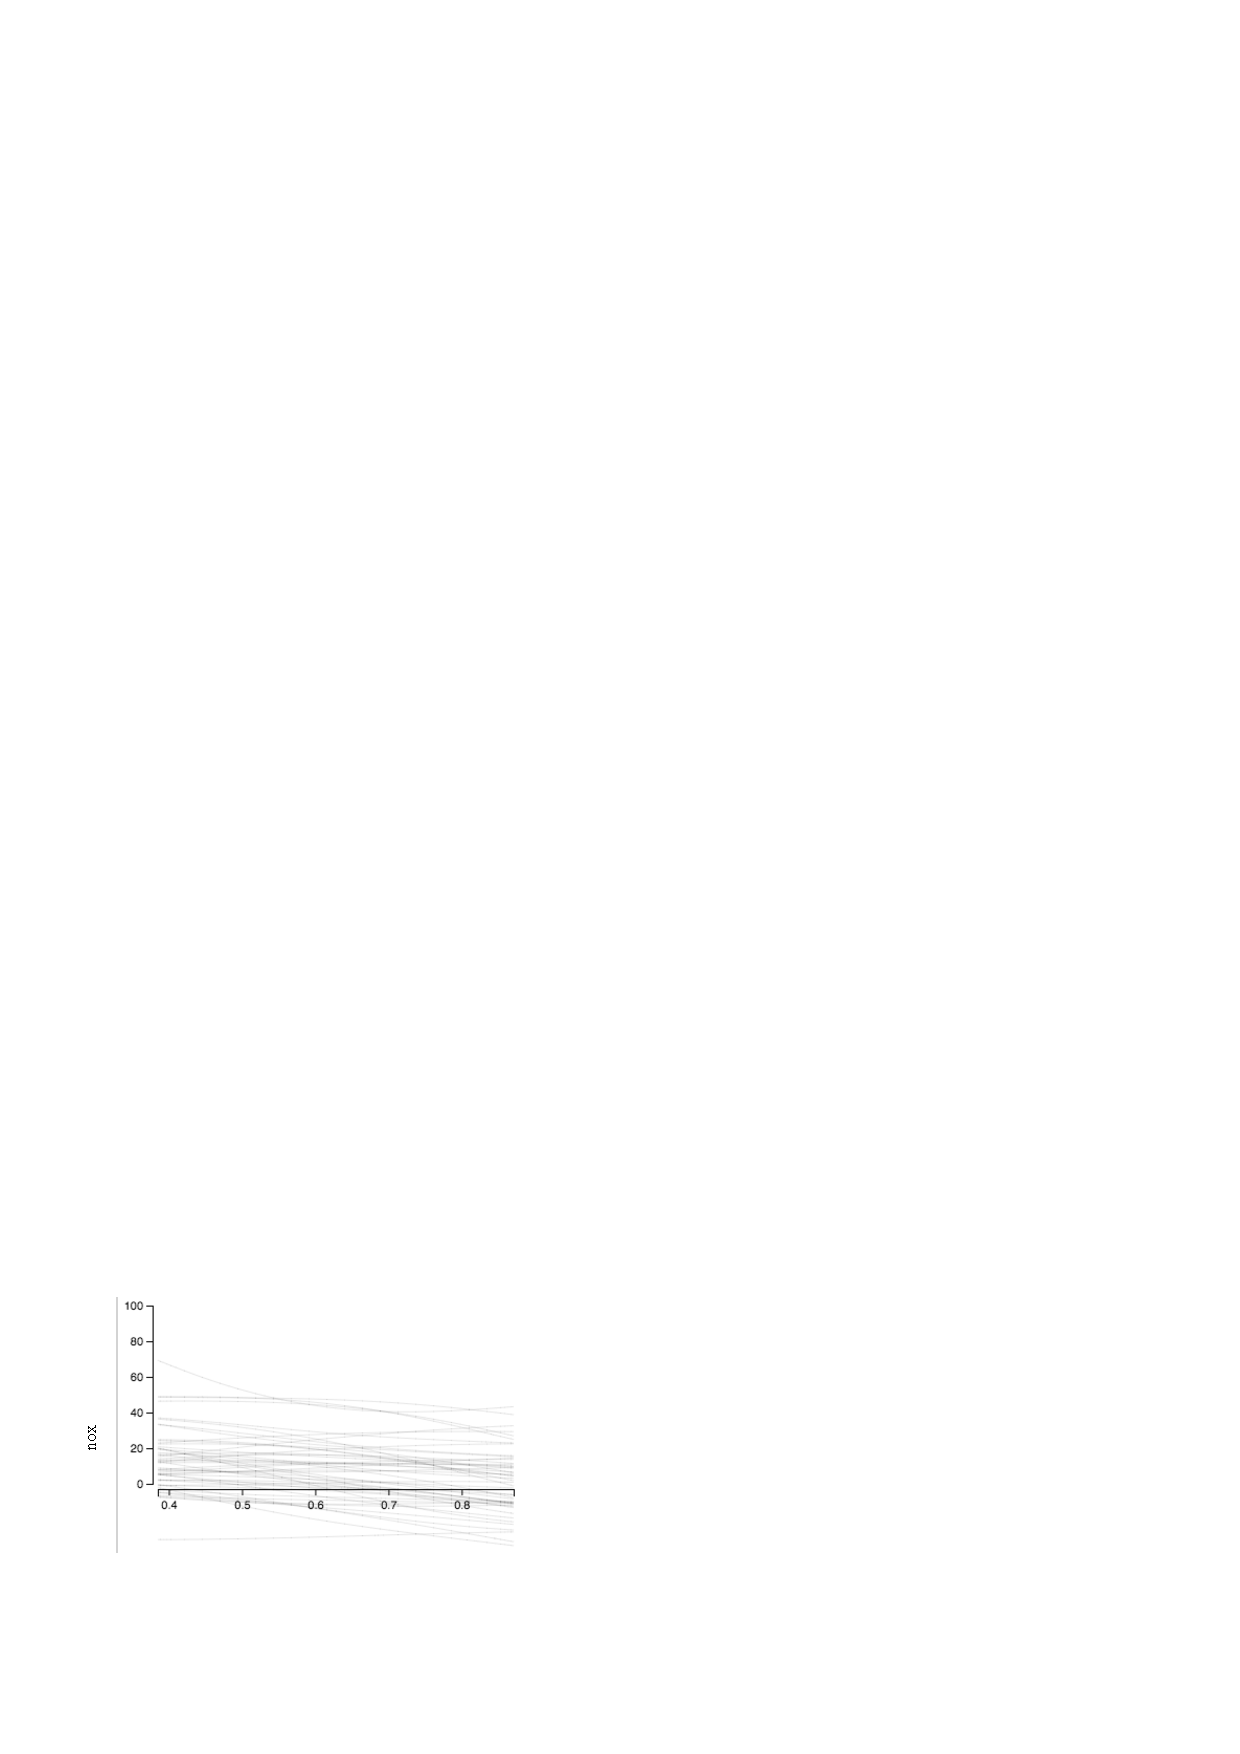
\includegraphics[width=\textwidth]{nn26_5.pdf}
    \end{subfigure}
    &
    \begin{subfigure}[b]{0.2\textwidth}
      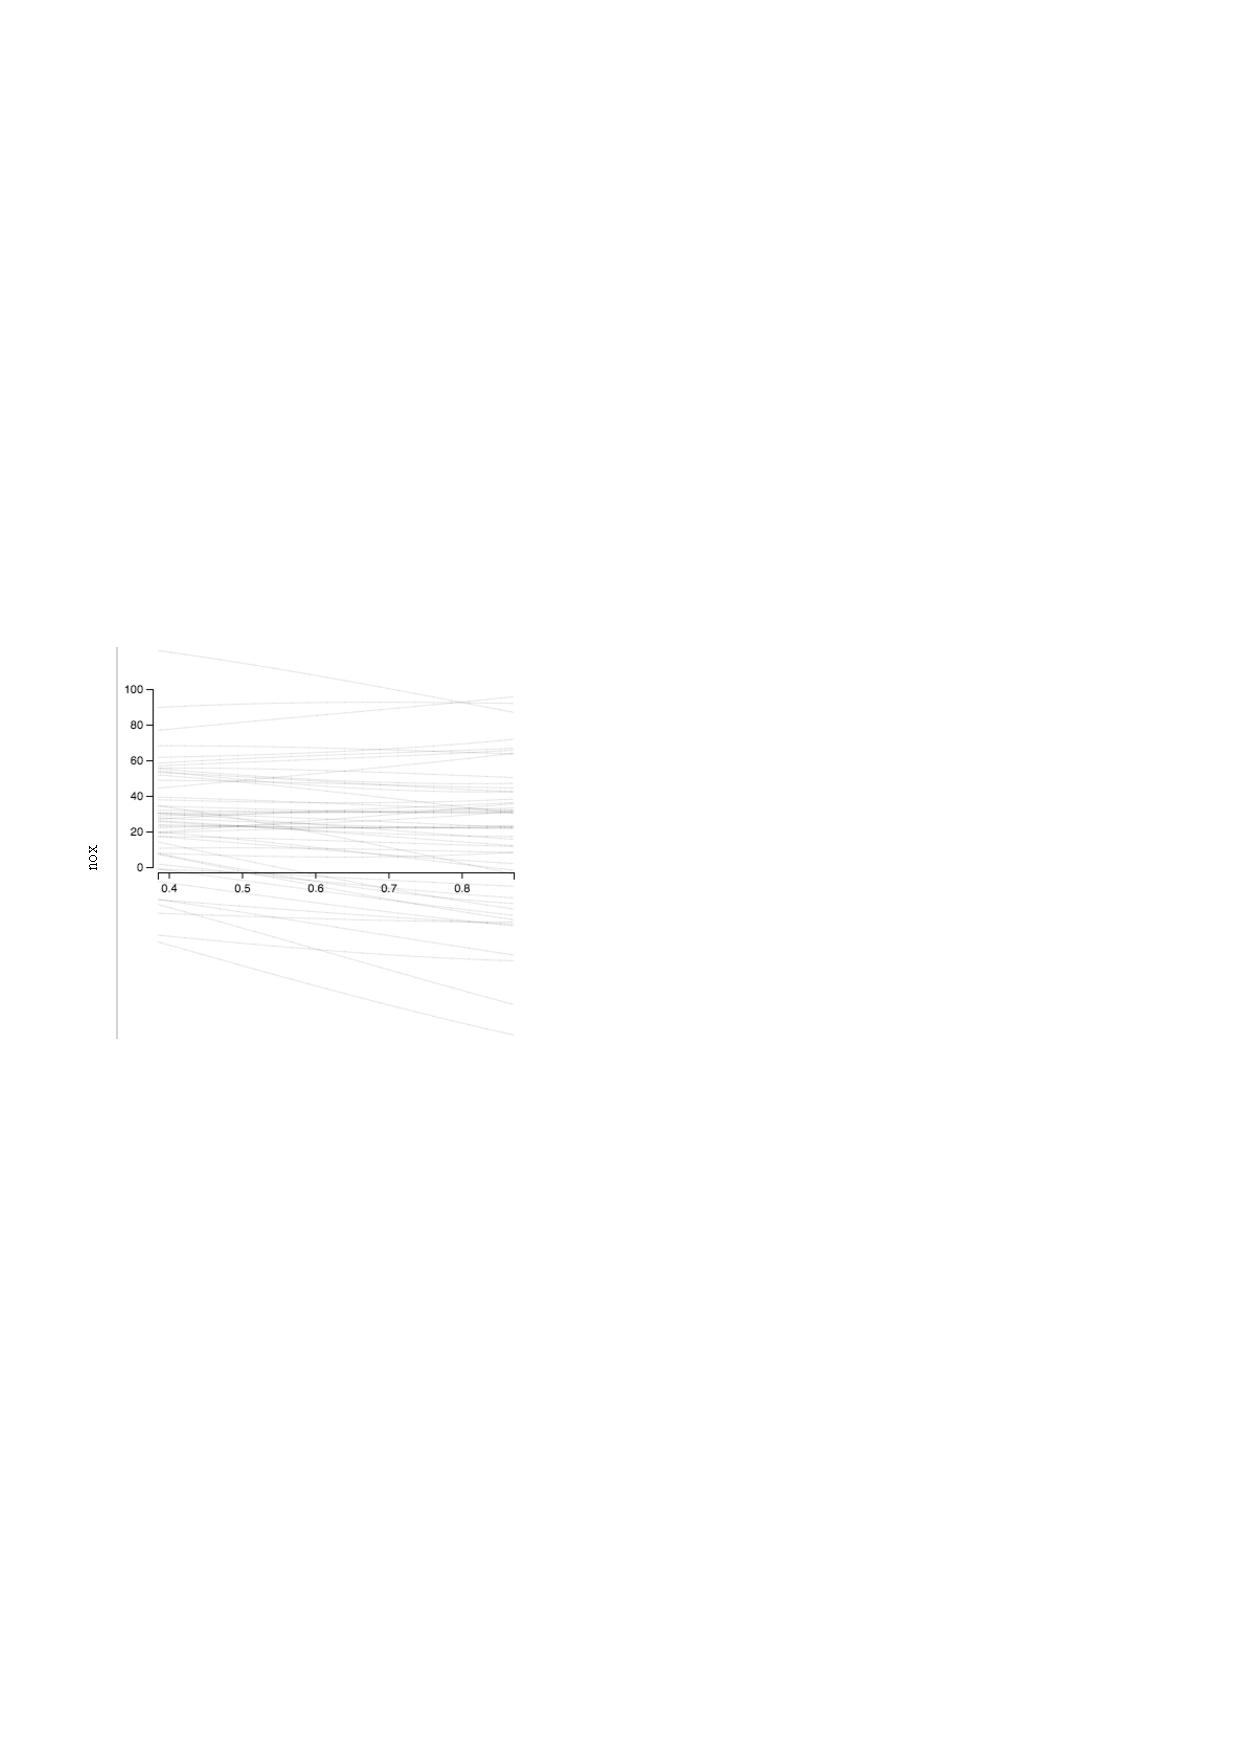
\includegraphics[width=\textwidth]{svmp_5.pdf}
    \end{subfigure}
    &
    \begin{subfigure}[b]{0.2\textwidth}
      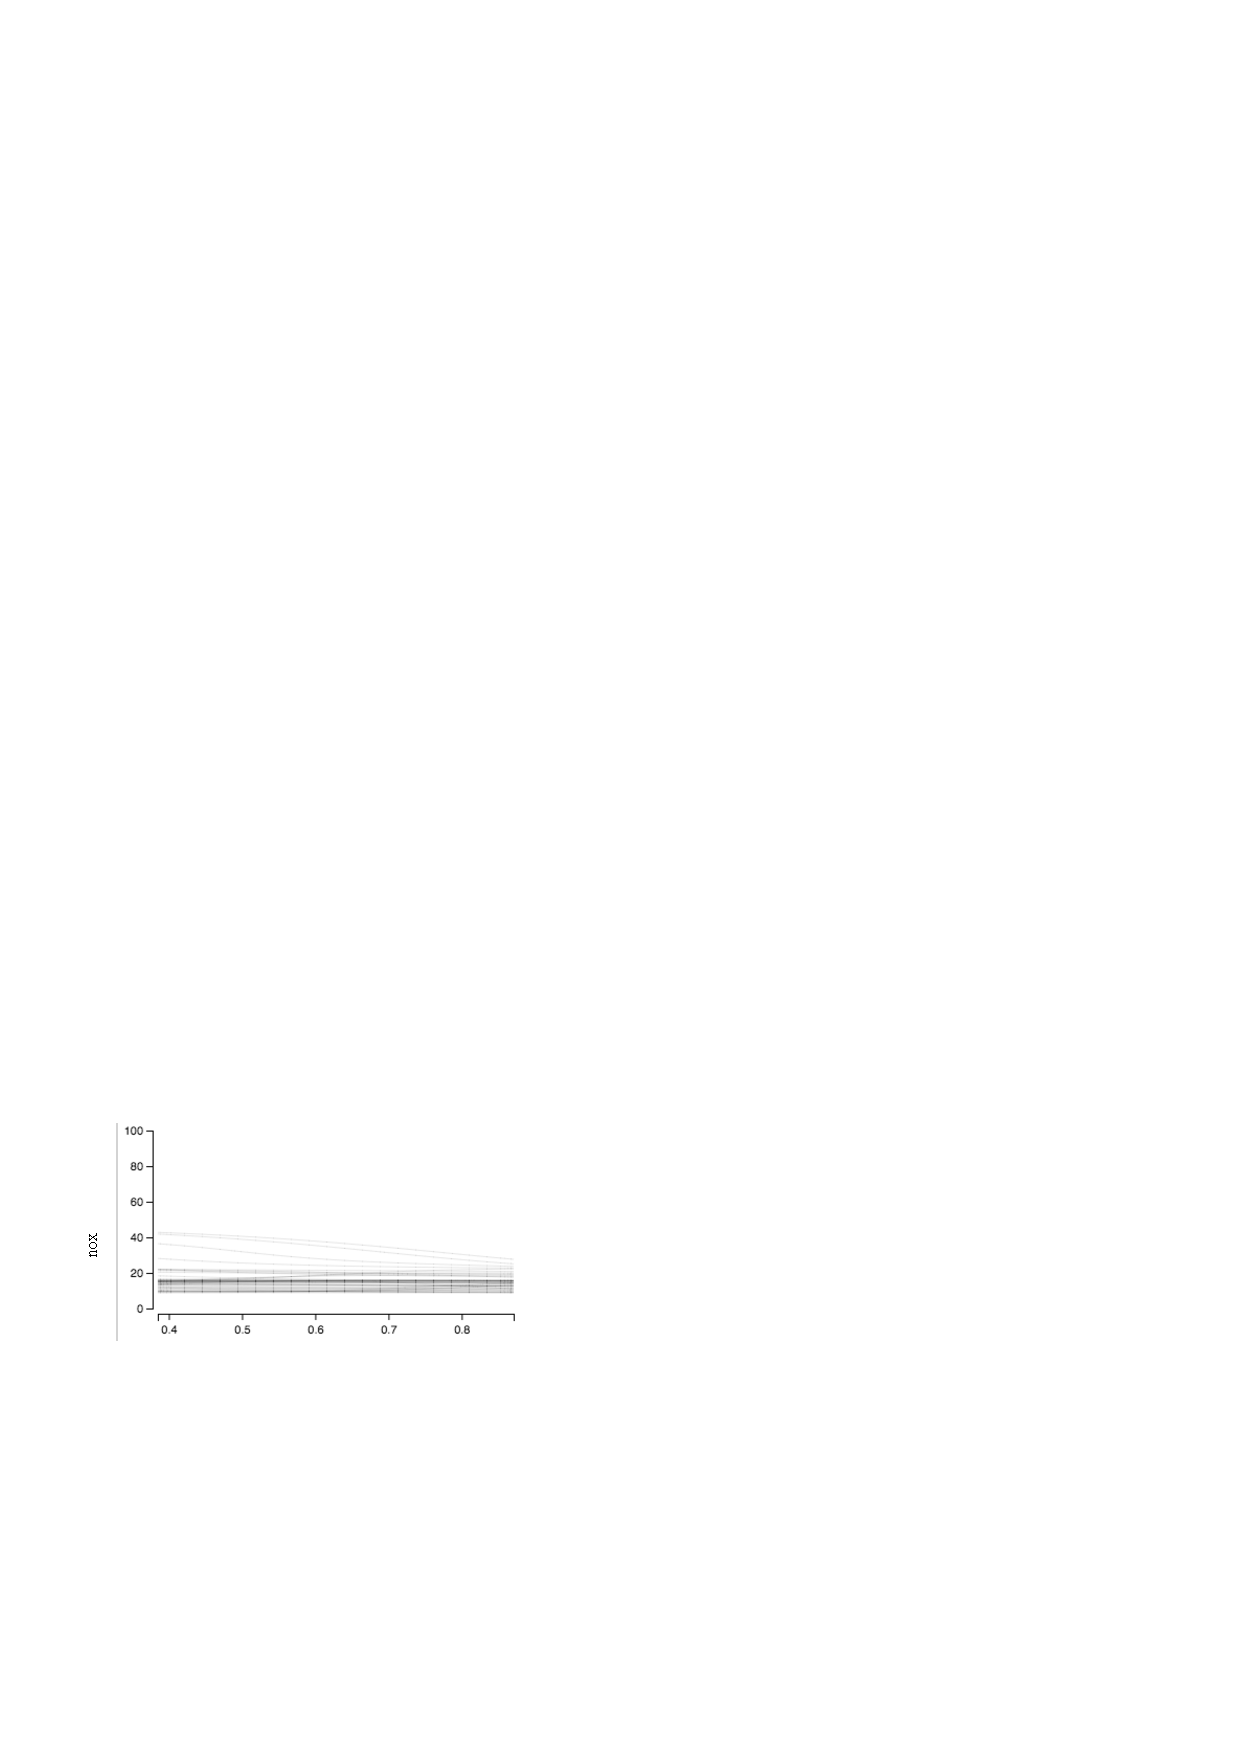
\includegraphics[width=\textwidth]{nn5x3_5.pdf}
    \end{subfigure}
    &
    \begin{subfigure}[b]{0.2\textwidth}
      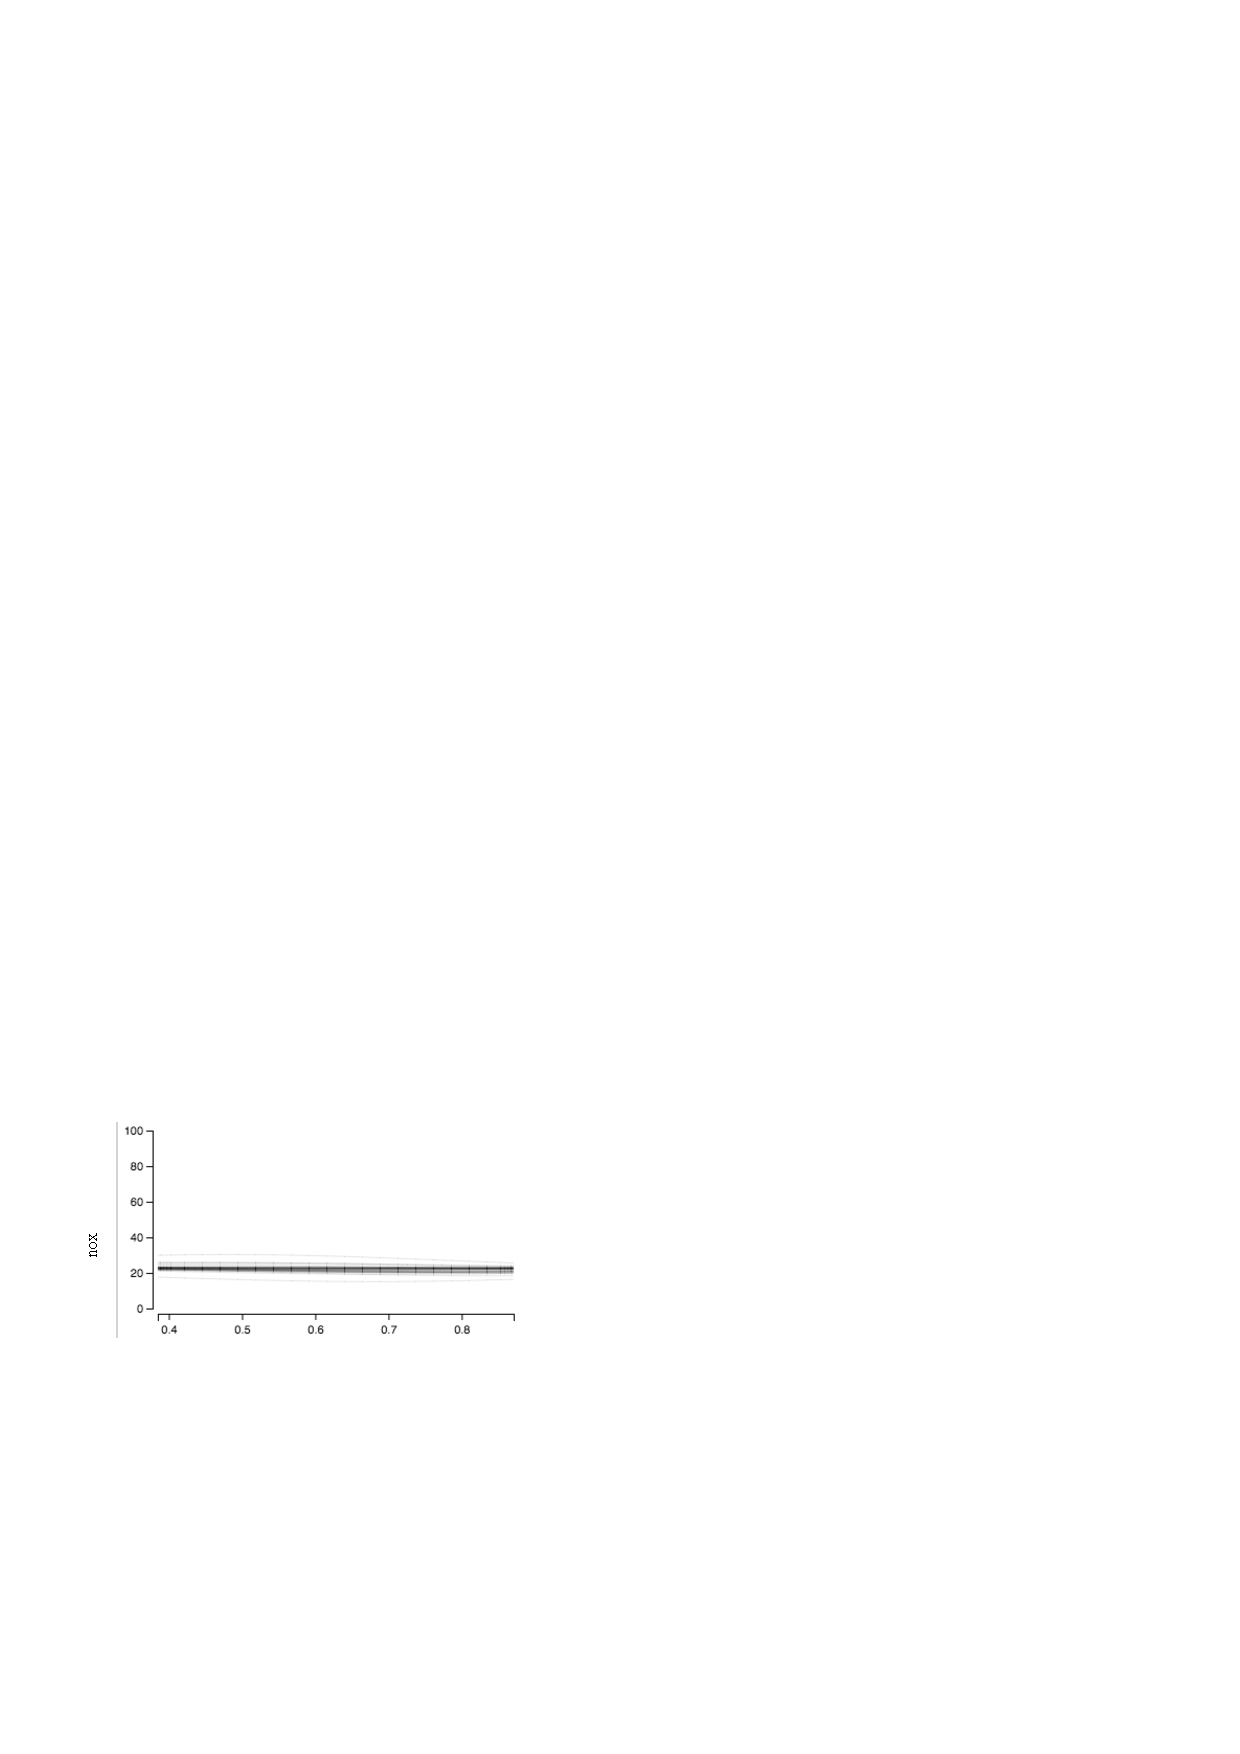
\includegraphics[width=\textwidth]{svmr_5.pdf}
    \end{subfigure}
    \\
    \hline \\
    Average number of rooms per dwelling &
    \begin{subfigure}[b]{0.2\textwidth}
      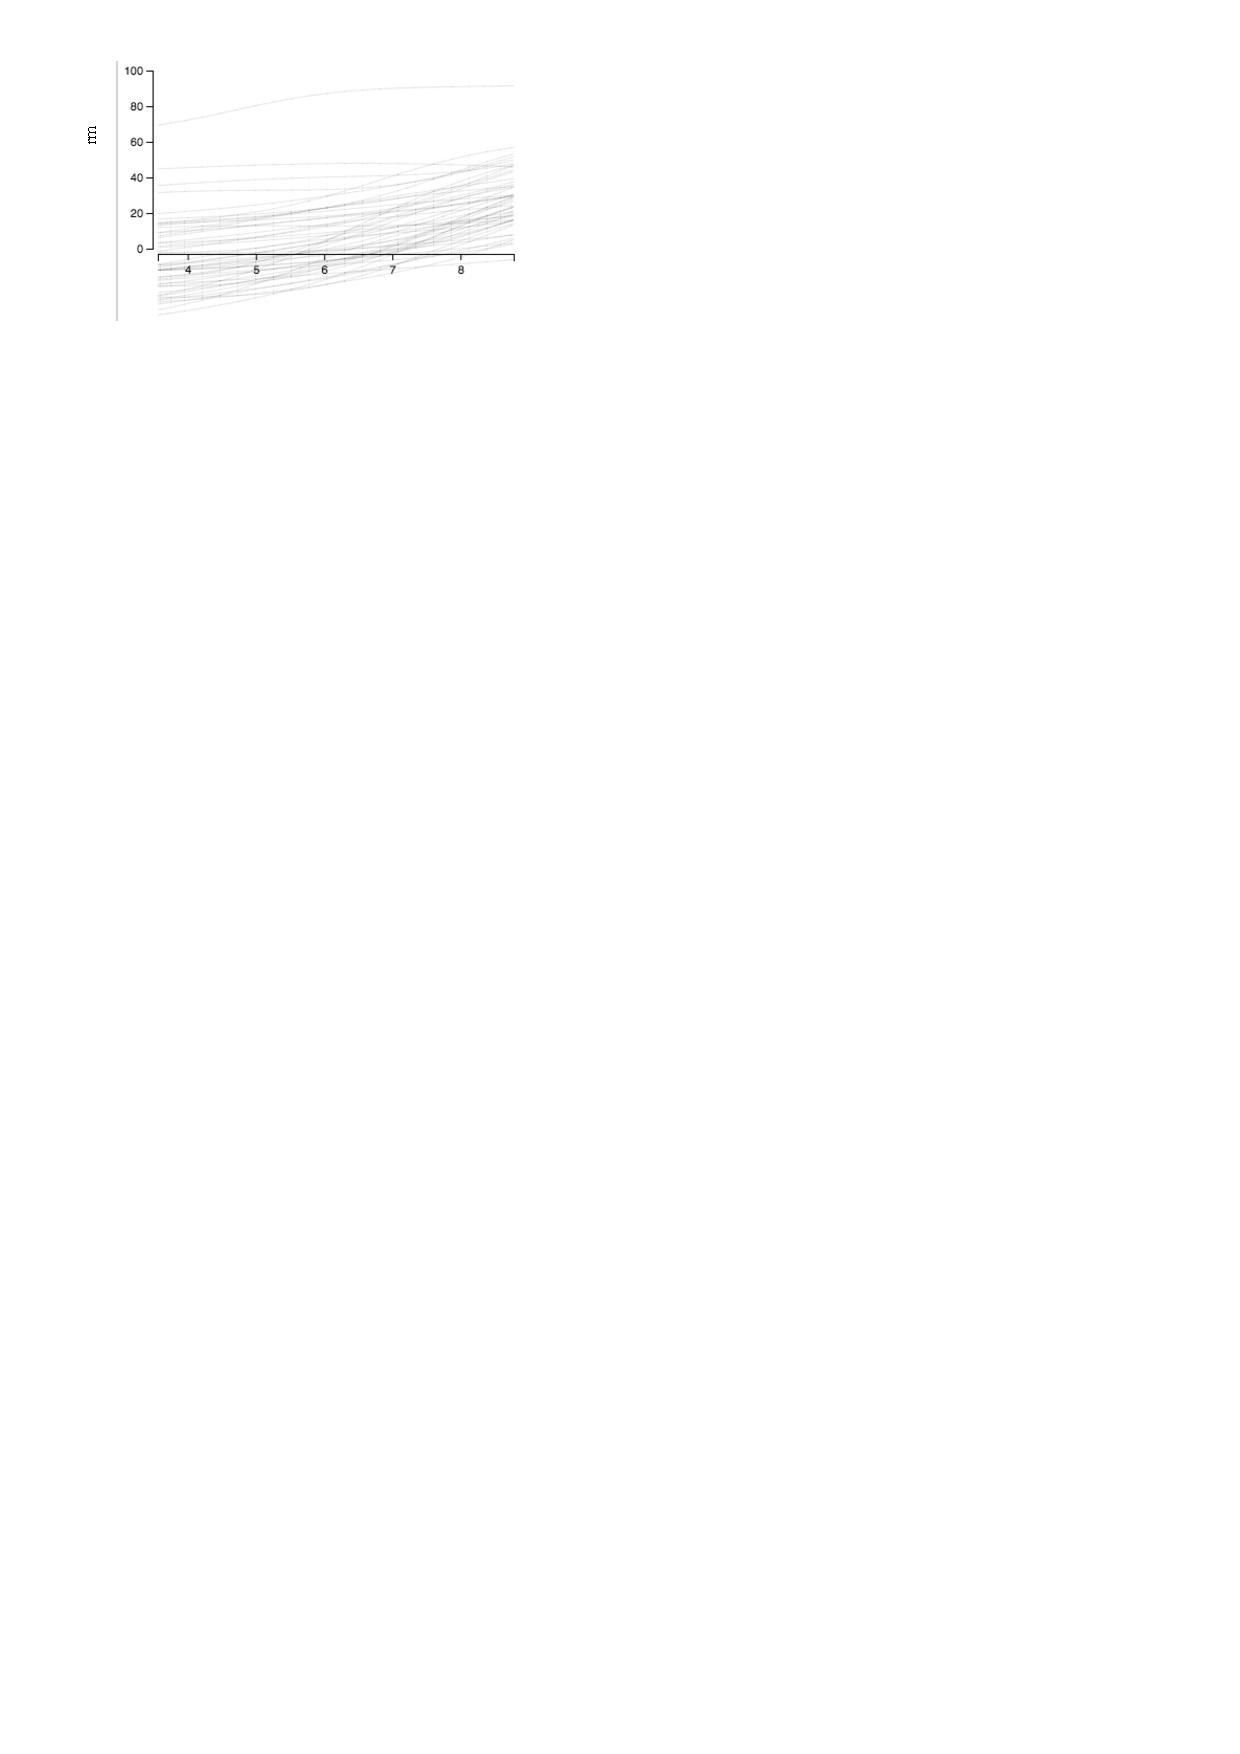
\includegraphics[width=\textwidth]{nn26_6.pdf}
    \end{subfigure}
    &
    \begin{subfigure}[b]{0.2\textwidth}
      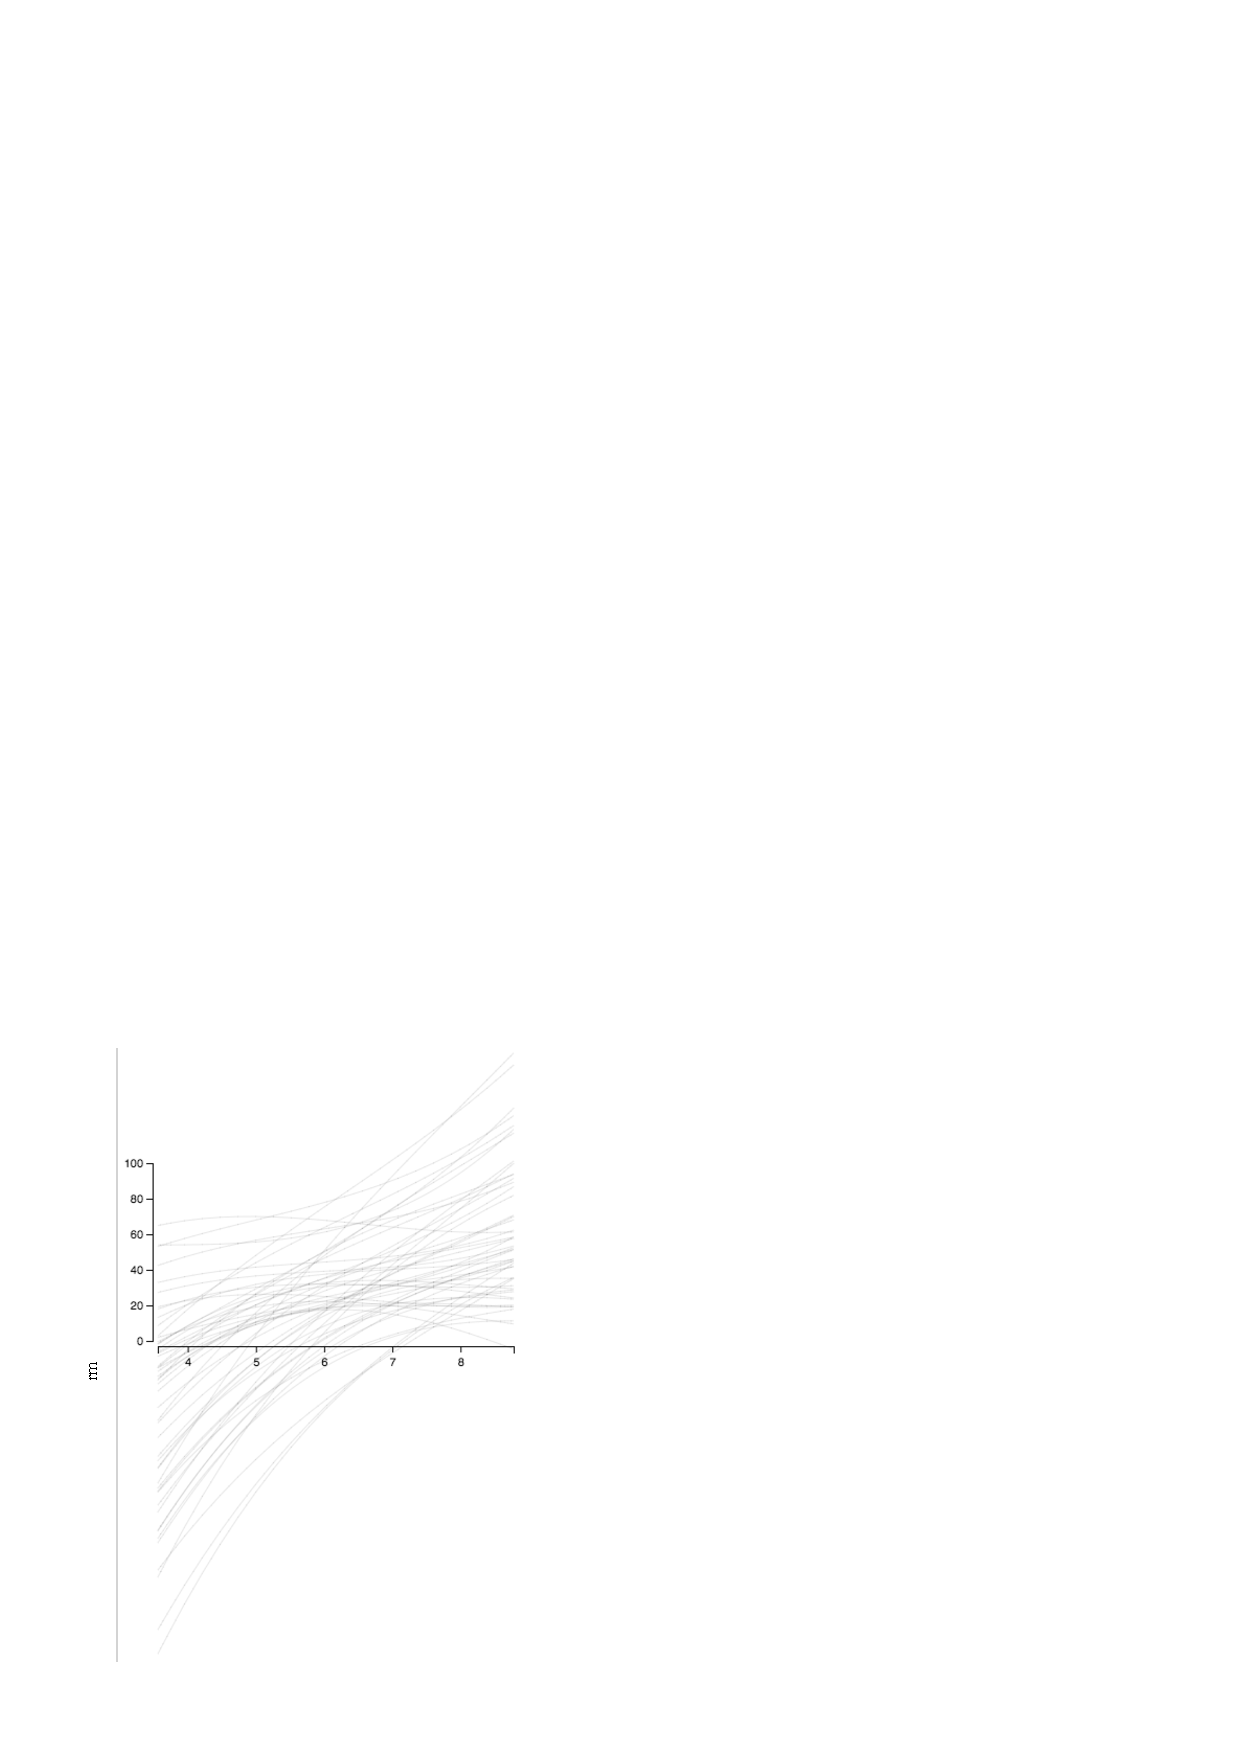
\includegraphics[width=\textwidth]{svmp_6.pdf}
    \end{subfigure}
    &
    \begin{subfigure}[b]{0.2\textwidth}
      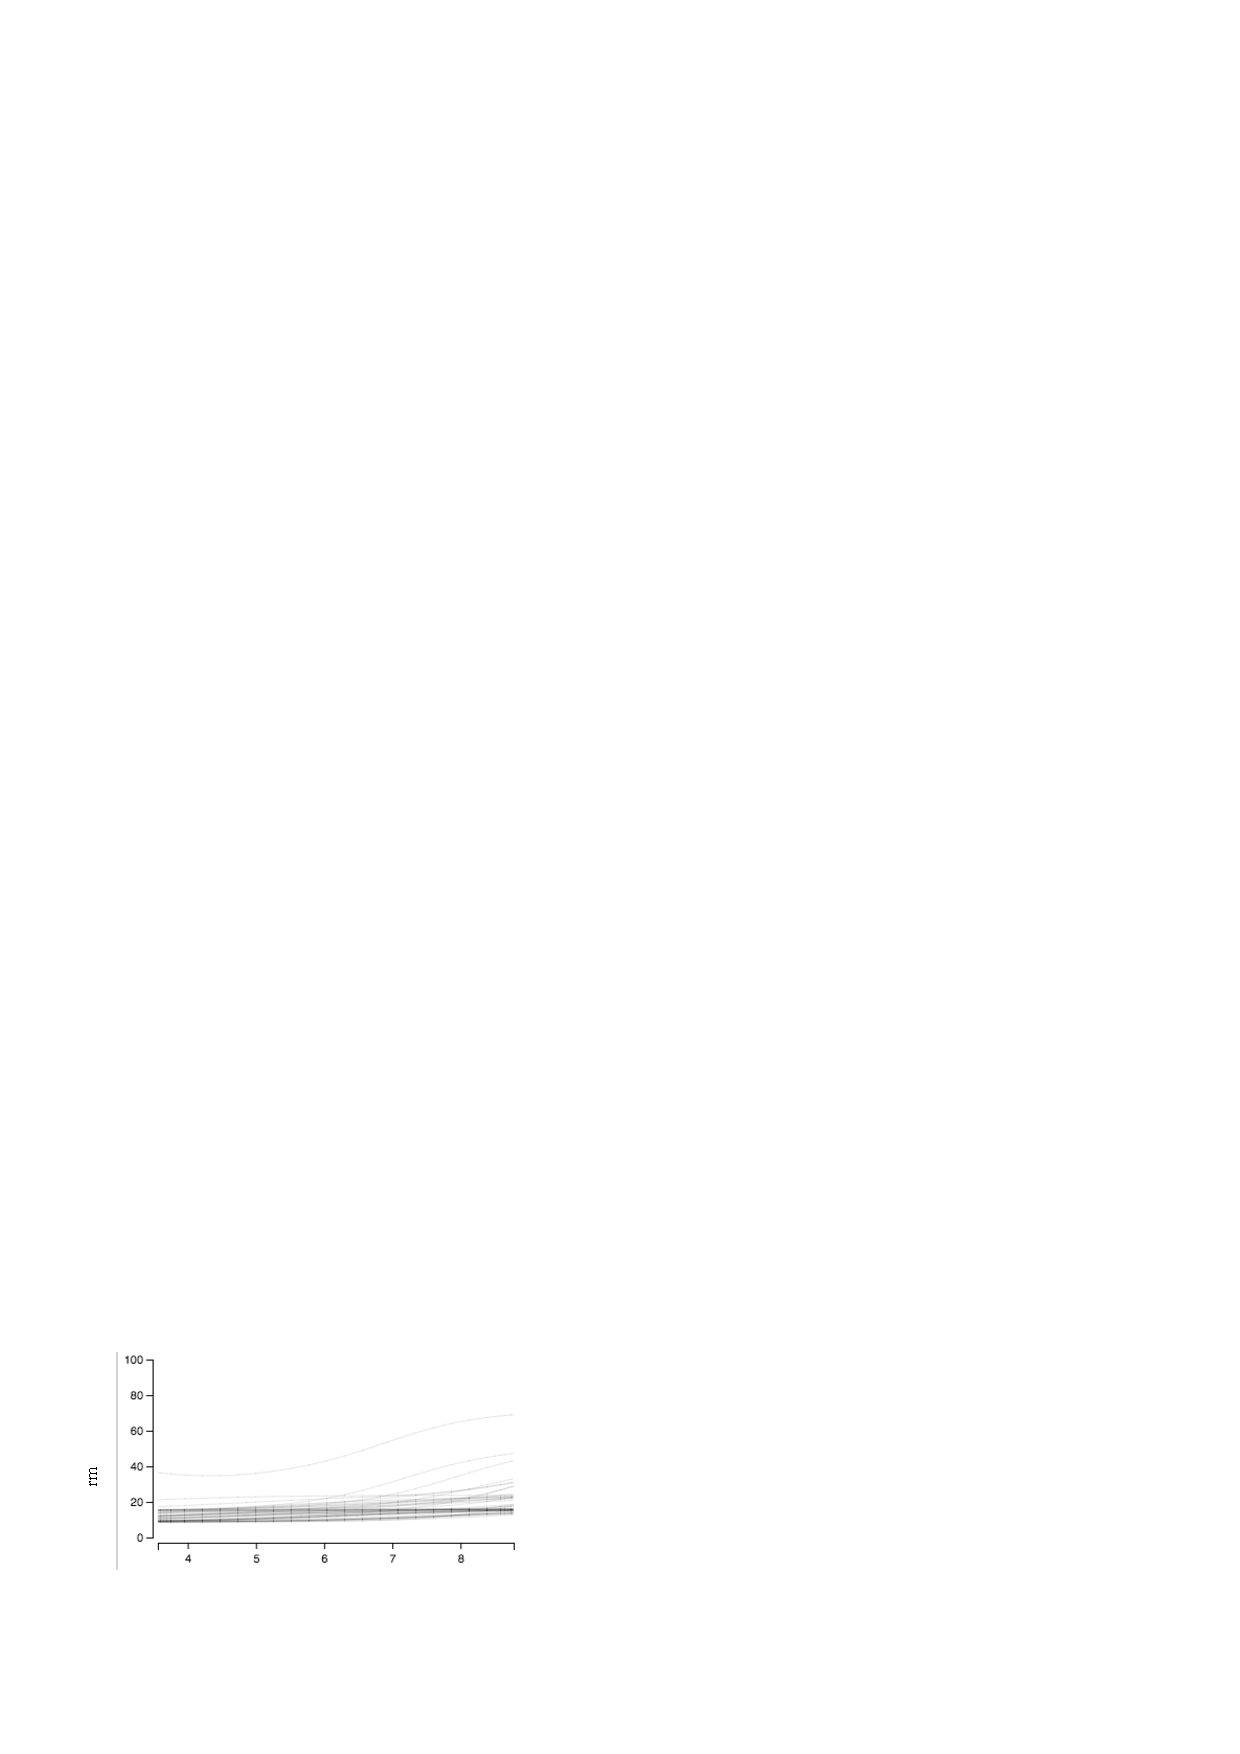
\includegraphics[width=\textwidth]{nn5x3_6.pdf}
    \end{subfigure}
    &
    \begin{subfigure}[b]{0.2\textwidth}
      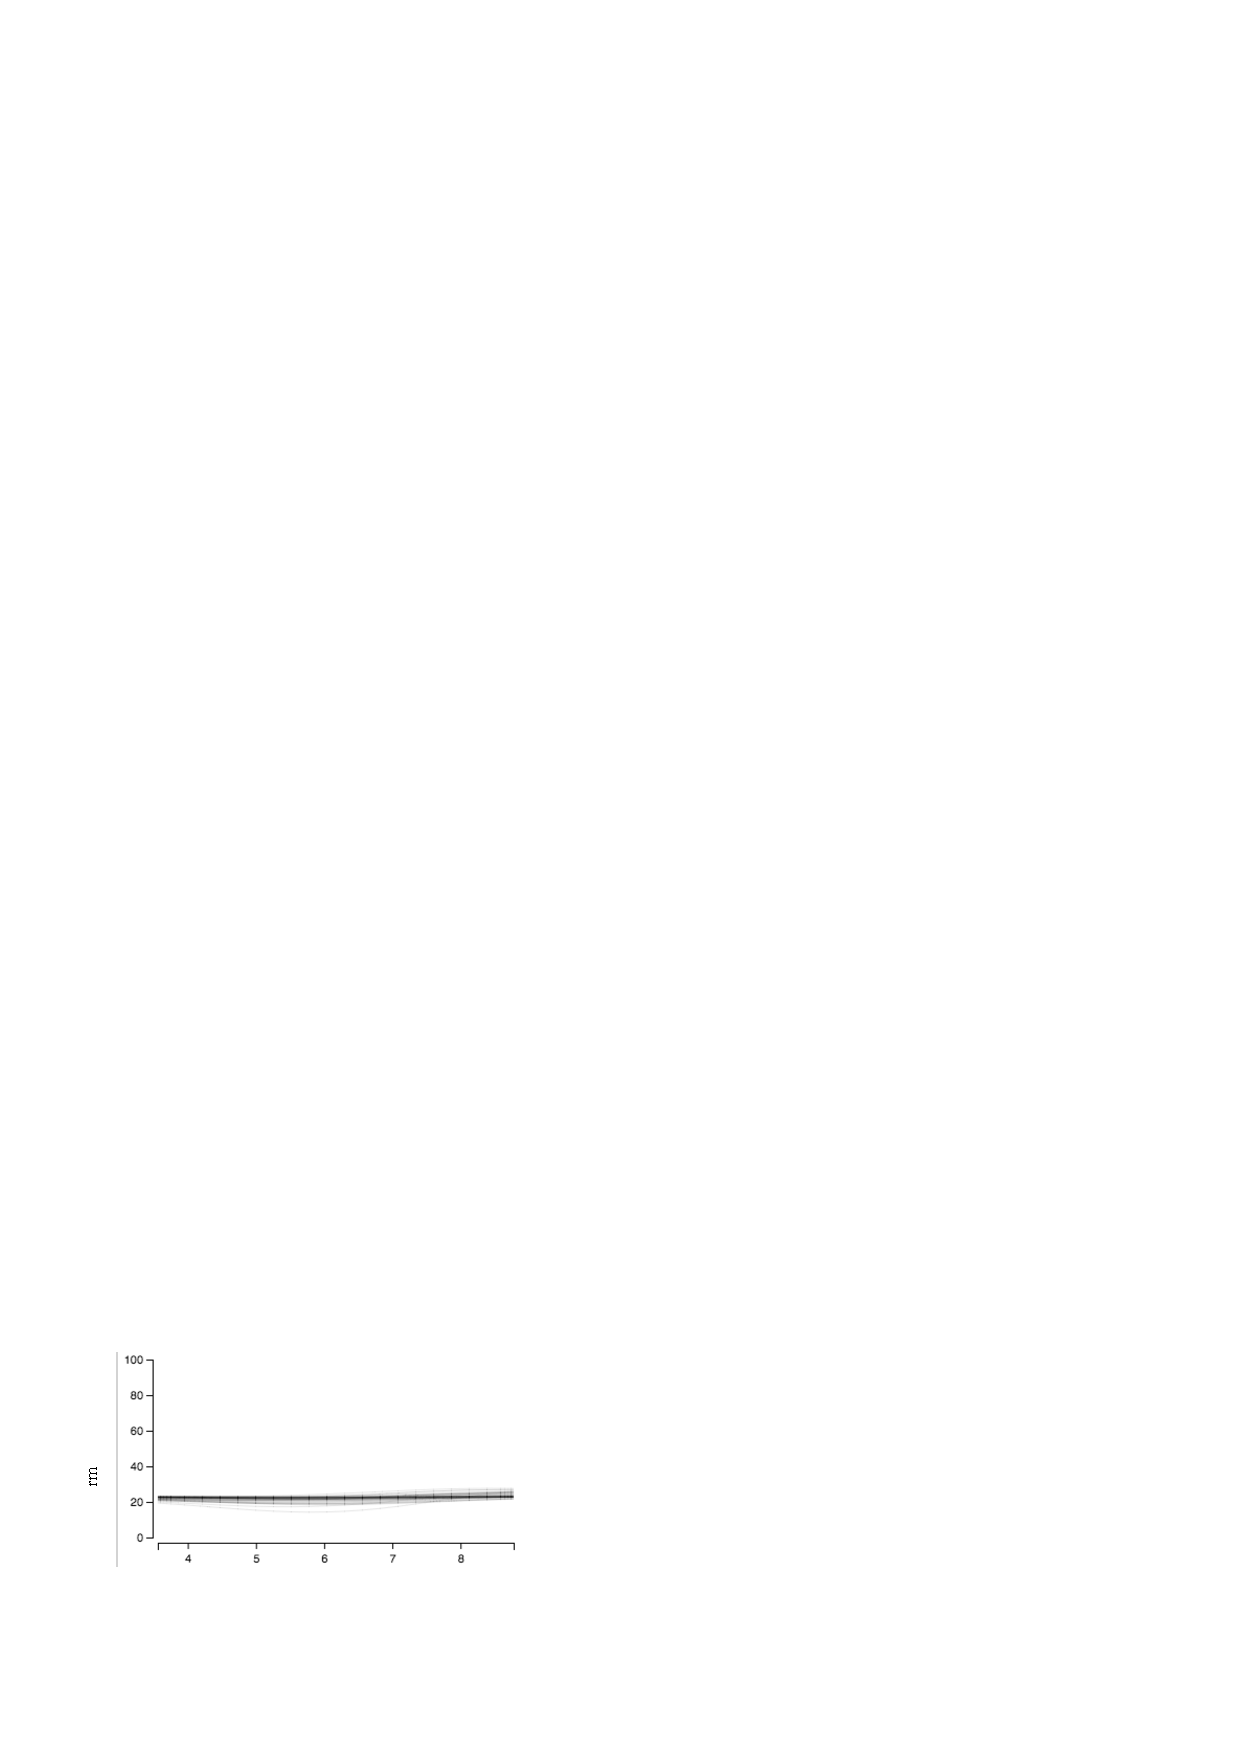
\includegraphics[width=\textwidth]{svmr_6.pdf}
    \end{subfigure}
    \\
    \hline \\
    Units built prior to 1940 &
    \begin{subfigure}[b]{0.2\textwidth}
      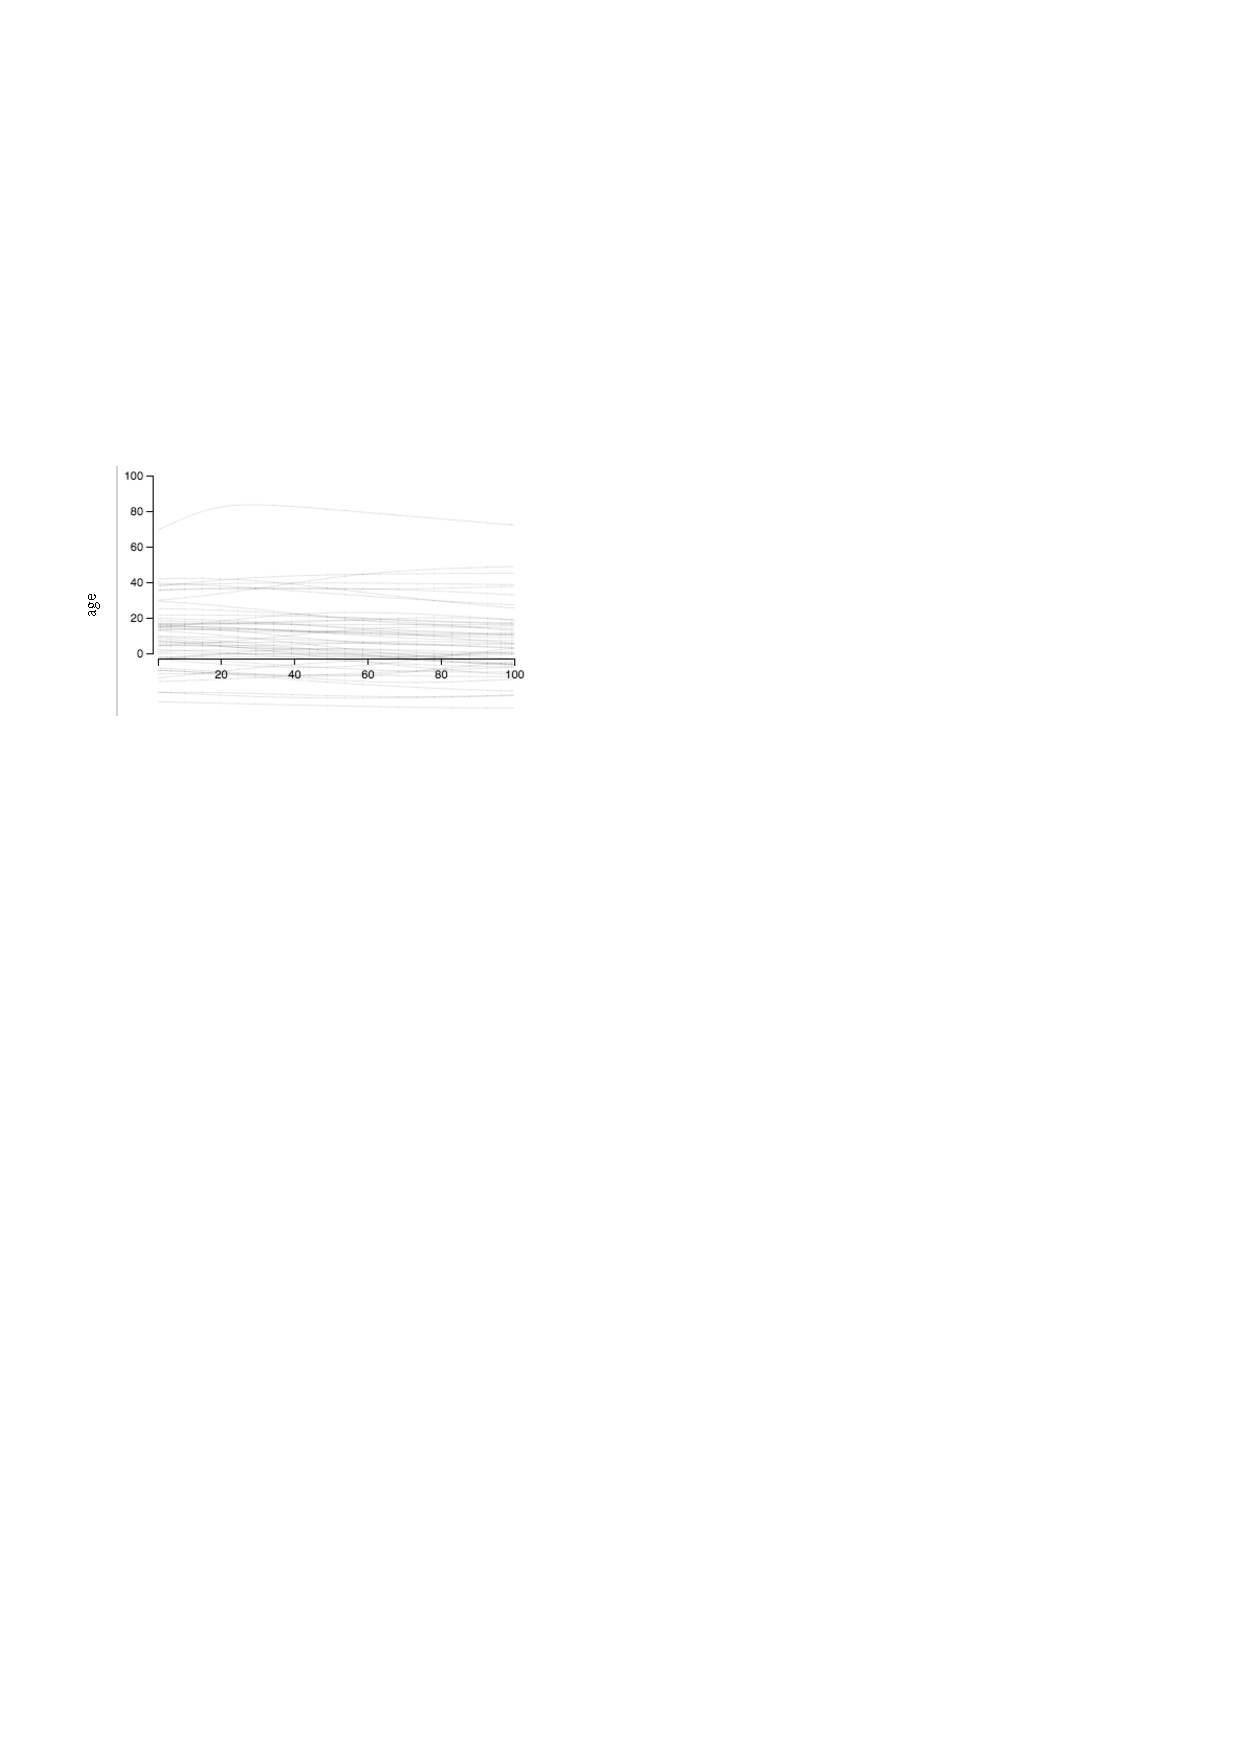
\includegraphics[width=\textwidth]{nn26_7.pdf}
    \end{subfigure}
    &
    \begin{subfigure}[b]{0.2\textwidth}
      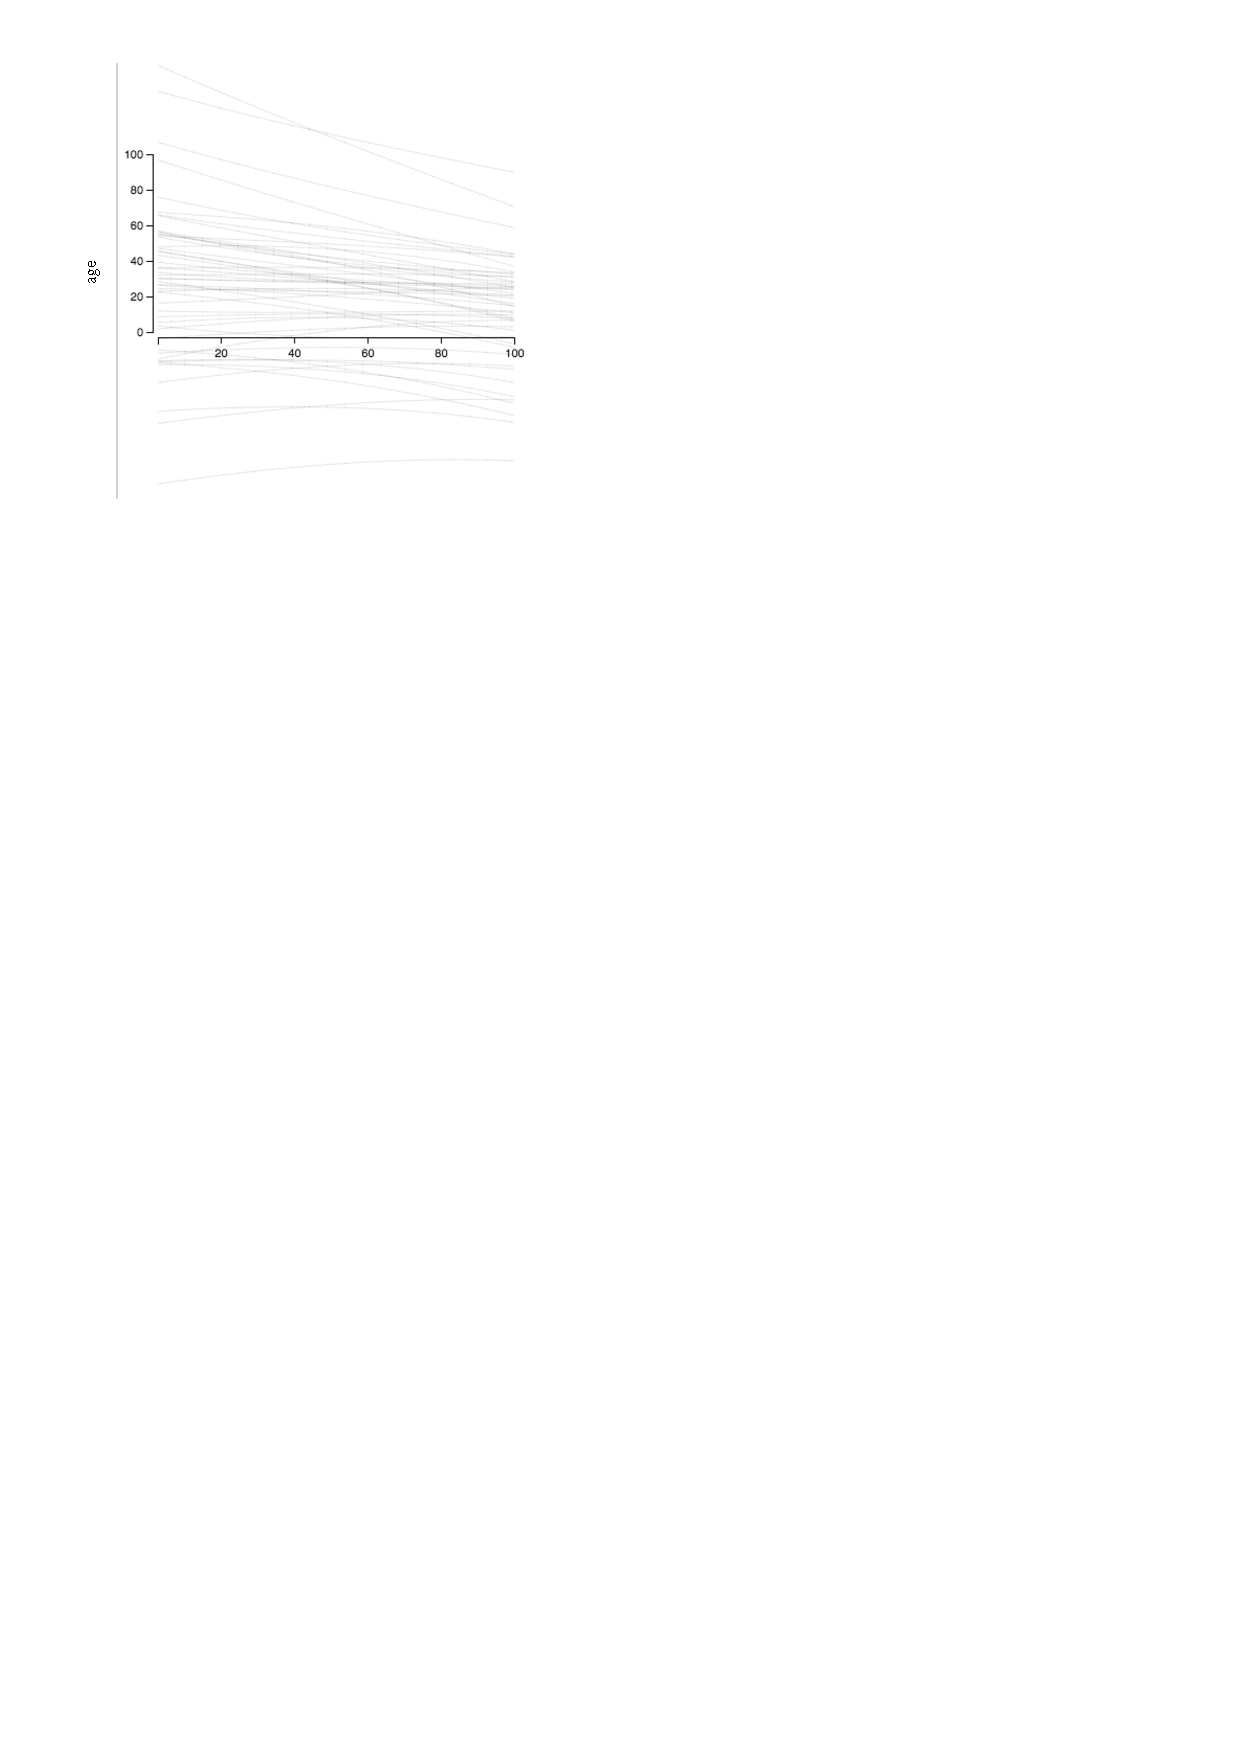
\includegraphics[width=\textwidth]{svmp_7.pdf}
    \end{subfigure}
    &
    \begin{subfigure}[b]{0.2\textwidth}
      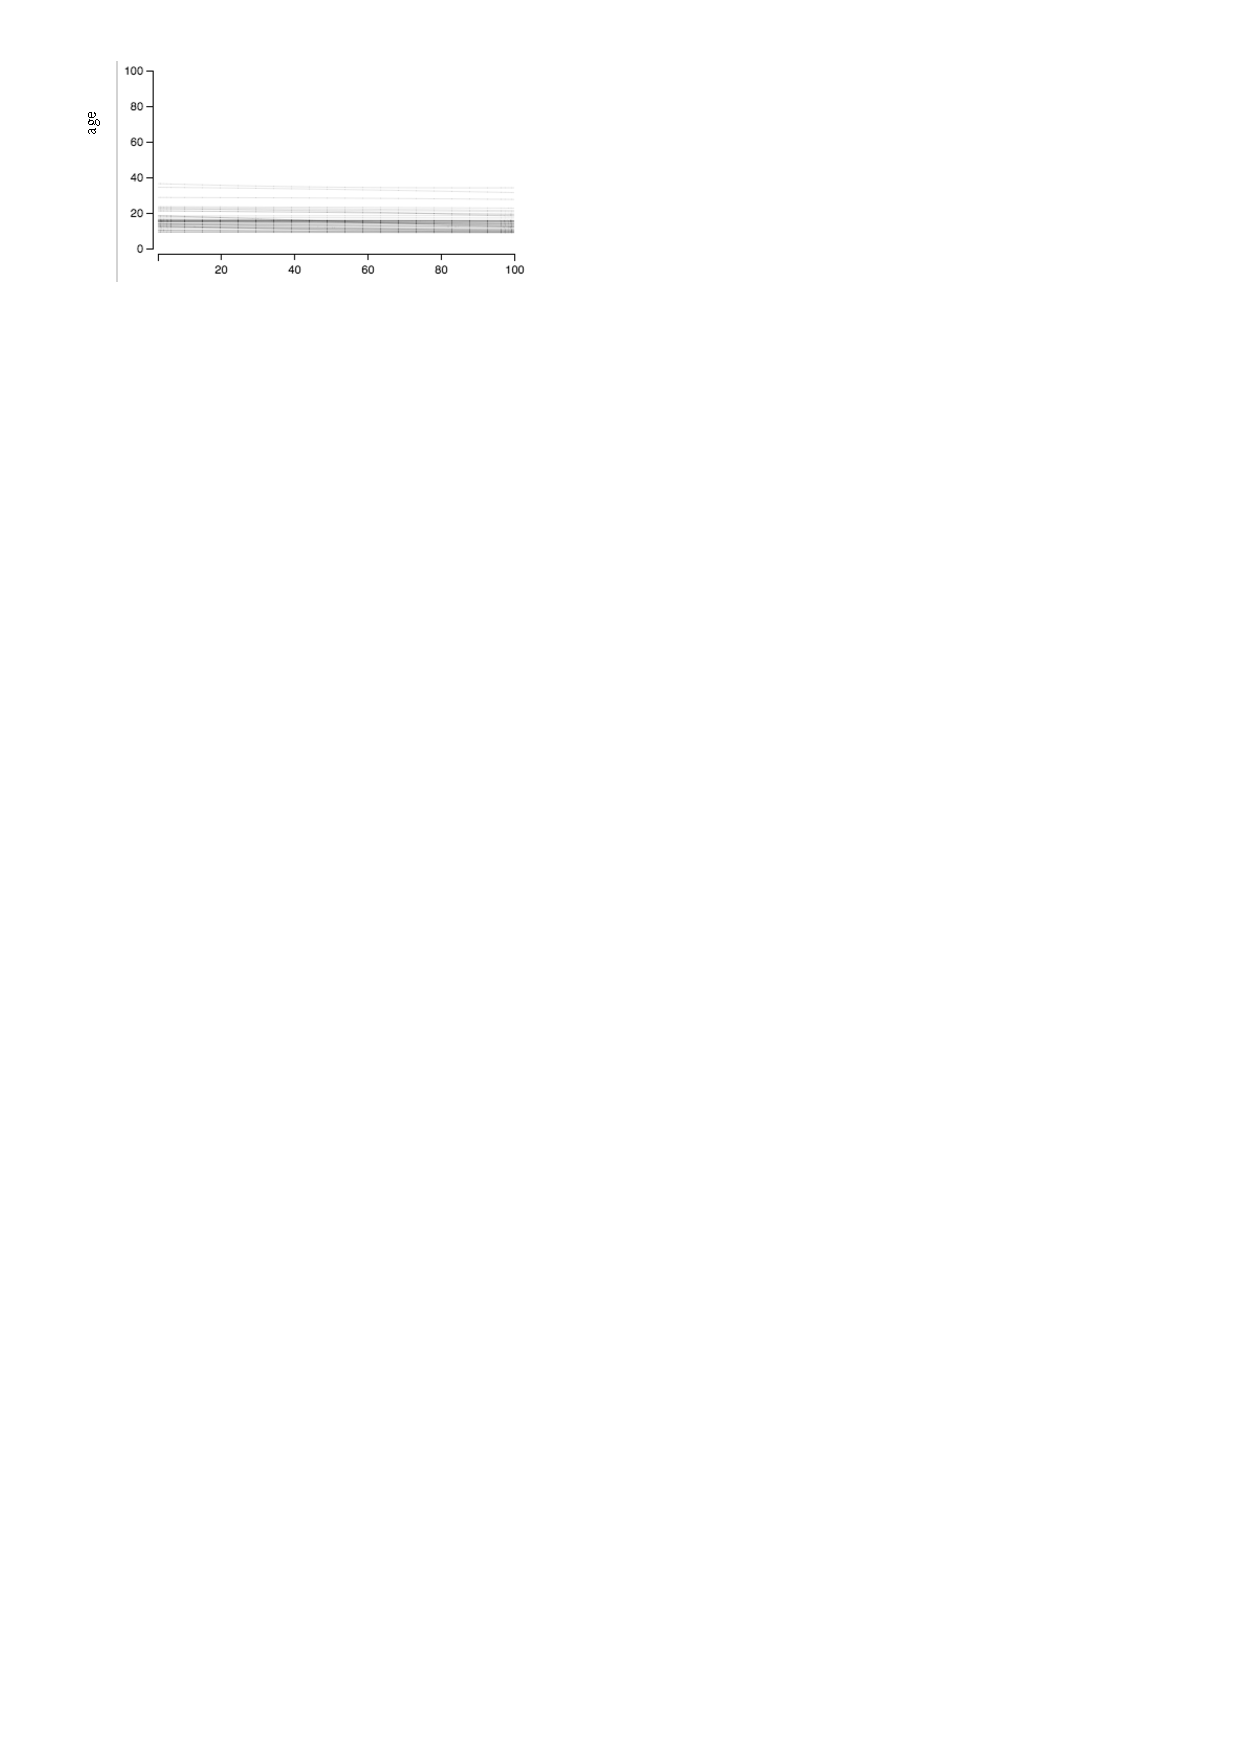
\includegraphics[width=\textwidth]{nn5x3_7.pdf}
    \end{subfigure}
    &
    \begin{subfigure}[b]{0.2\textwidth}
      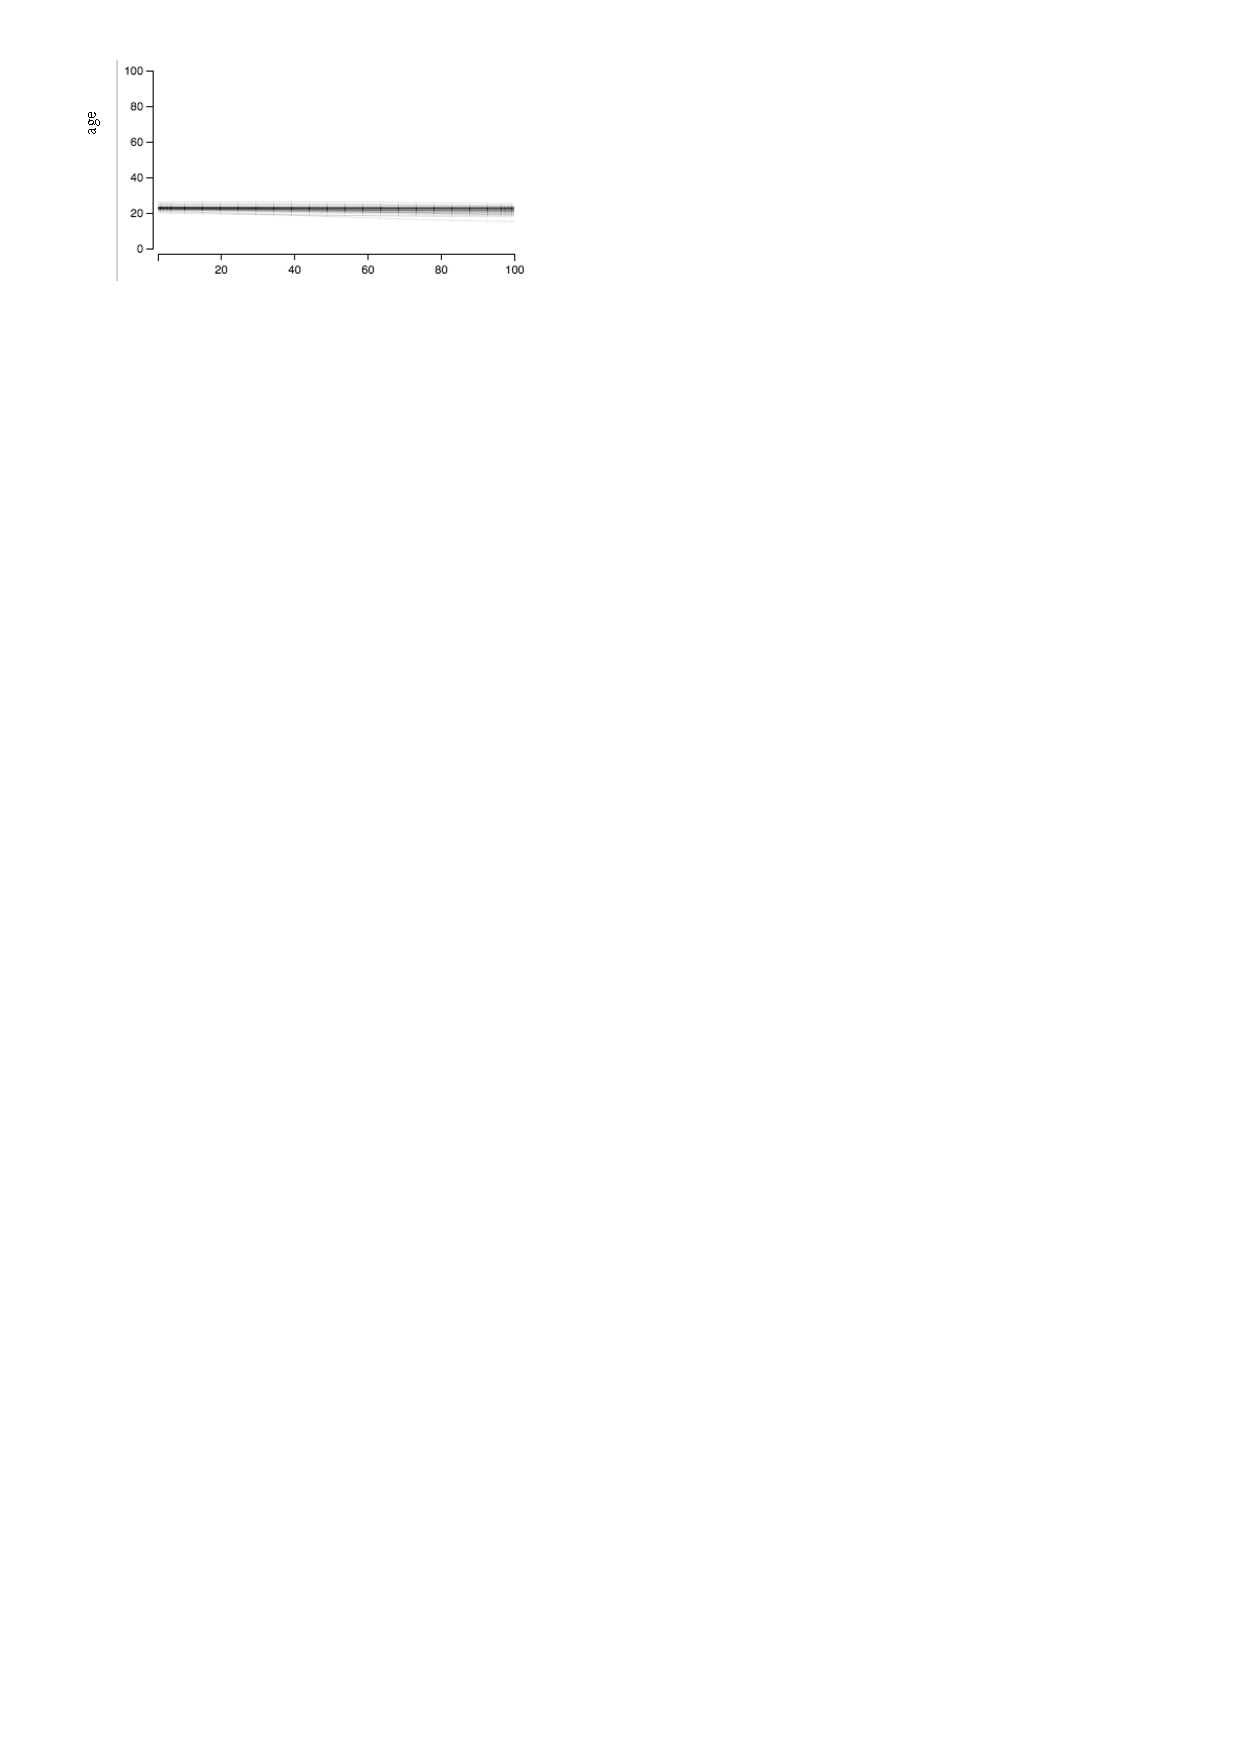
\includegraphics[width=\textwidth]{svmr_7.pdf}
    \end{subfigure}
    \\
    \hline \\
    Distances to employment centres &
    \begin{subfigure}[b]{0.2\textwidth}
      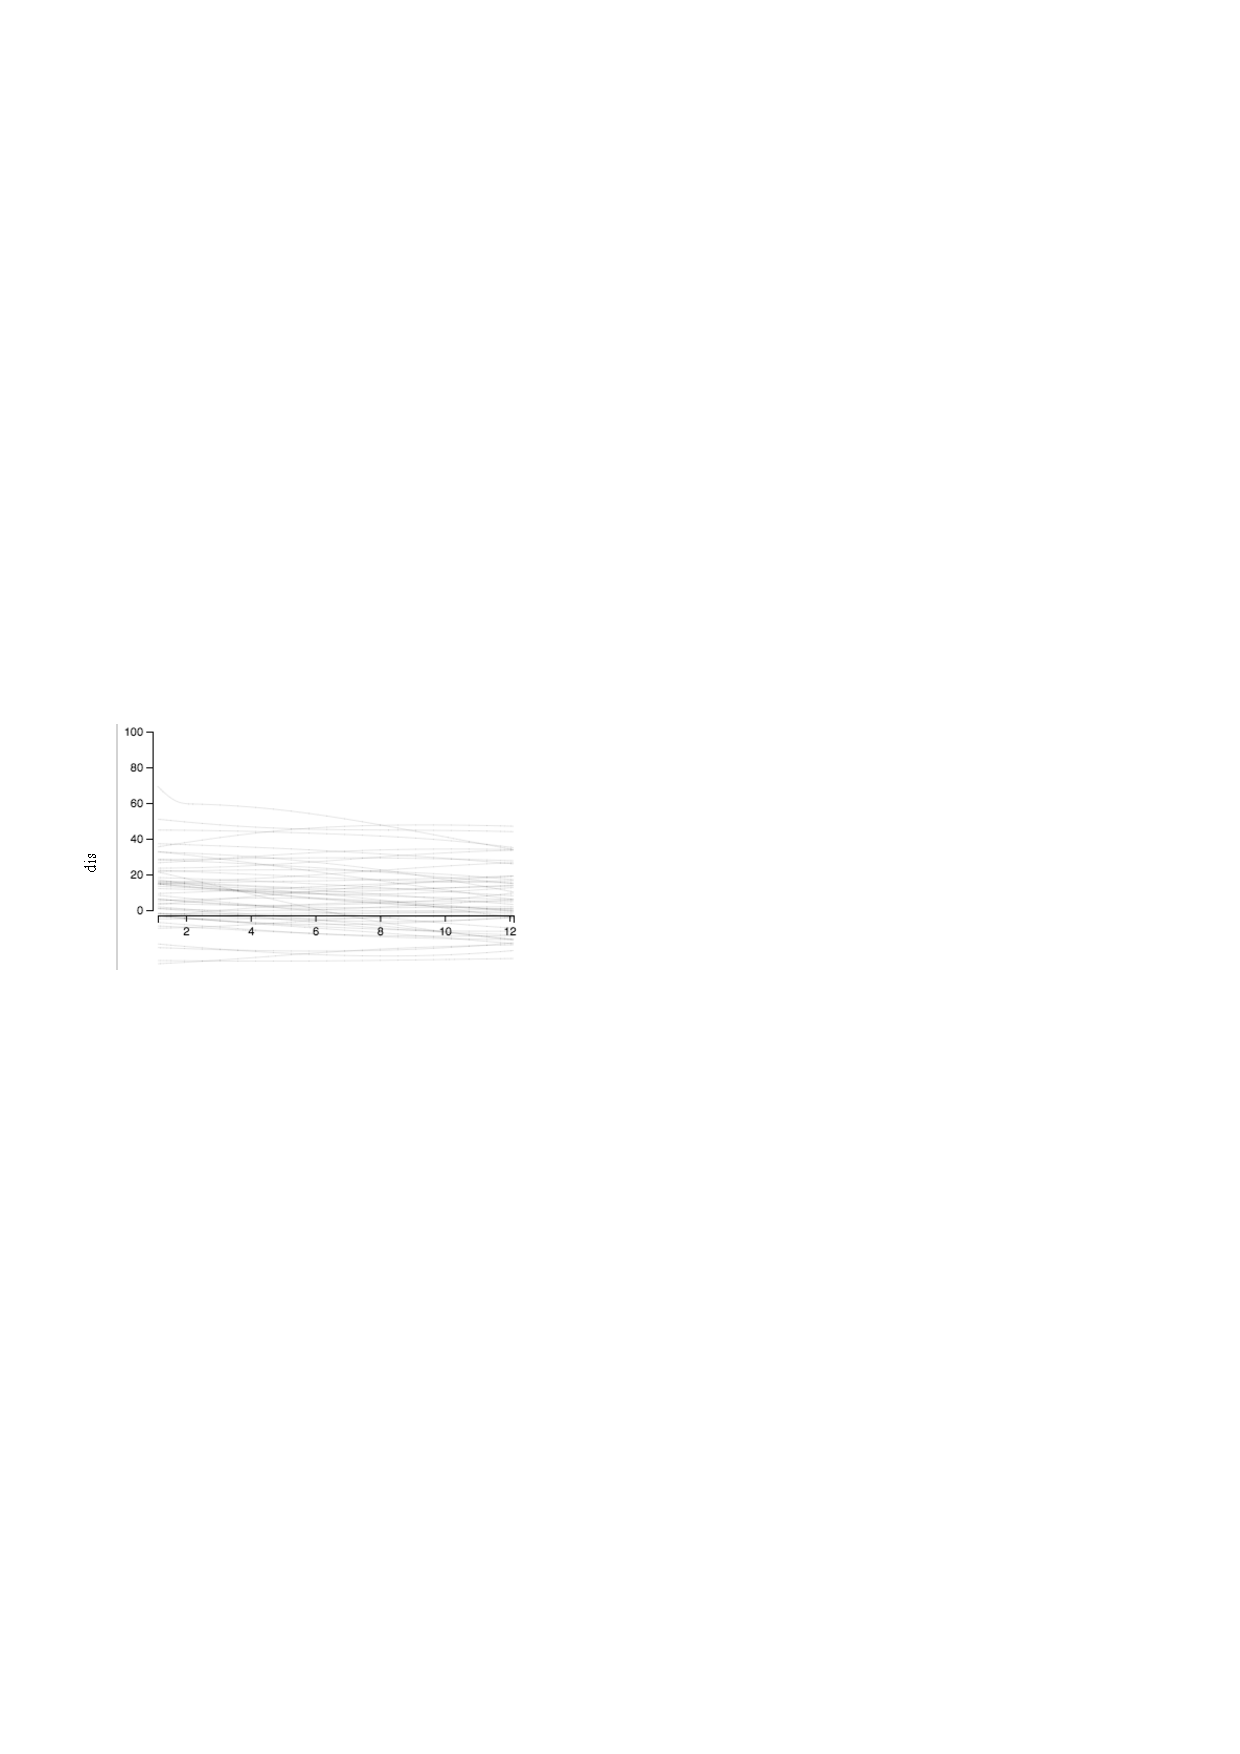
\includegraphics[width=\textwidth]{nn26_8.pdf}
    \end{subfigure}
    &
    \begin{subfigure}[b]{0.2\textwidth}
      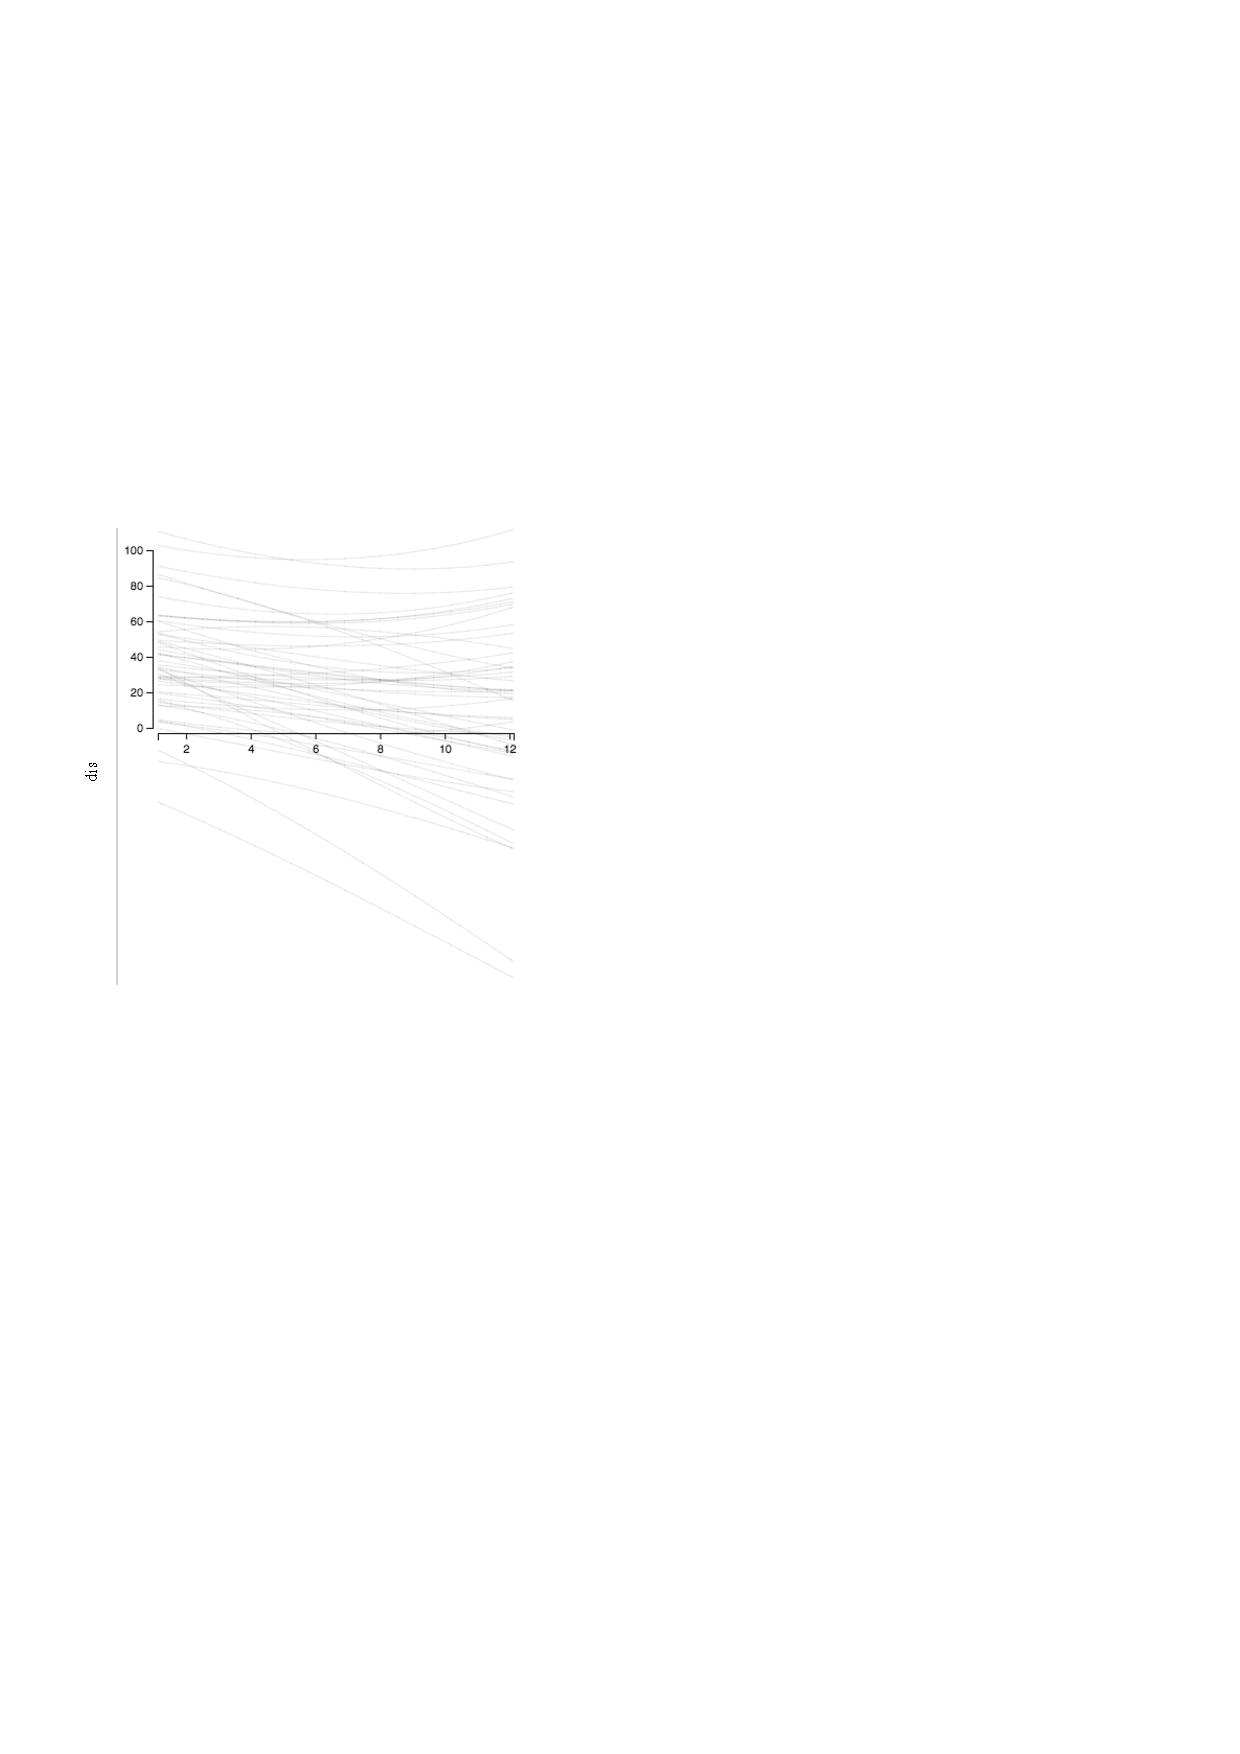
\includegraphics[width=\textwidth]{svmp_8.pdf}
    \end{subfigure}
    &
    \begin{subfigure}[b]{0.2\textwidth}
      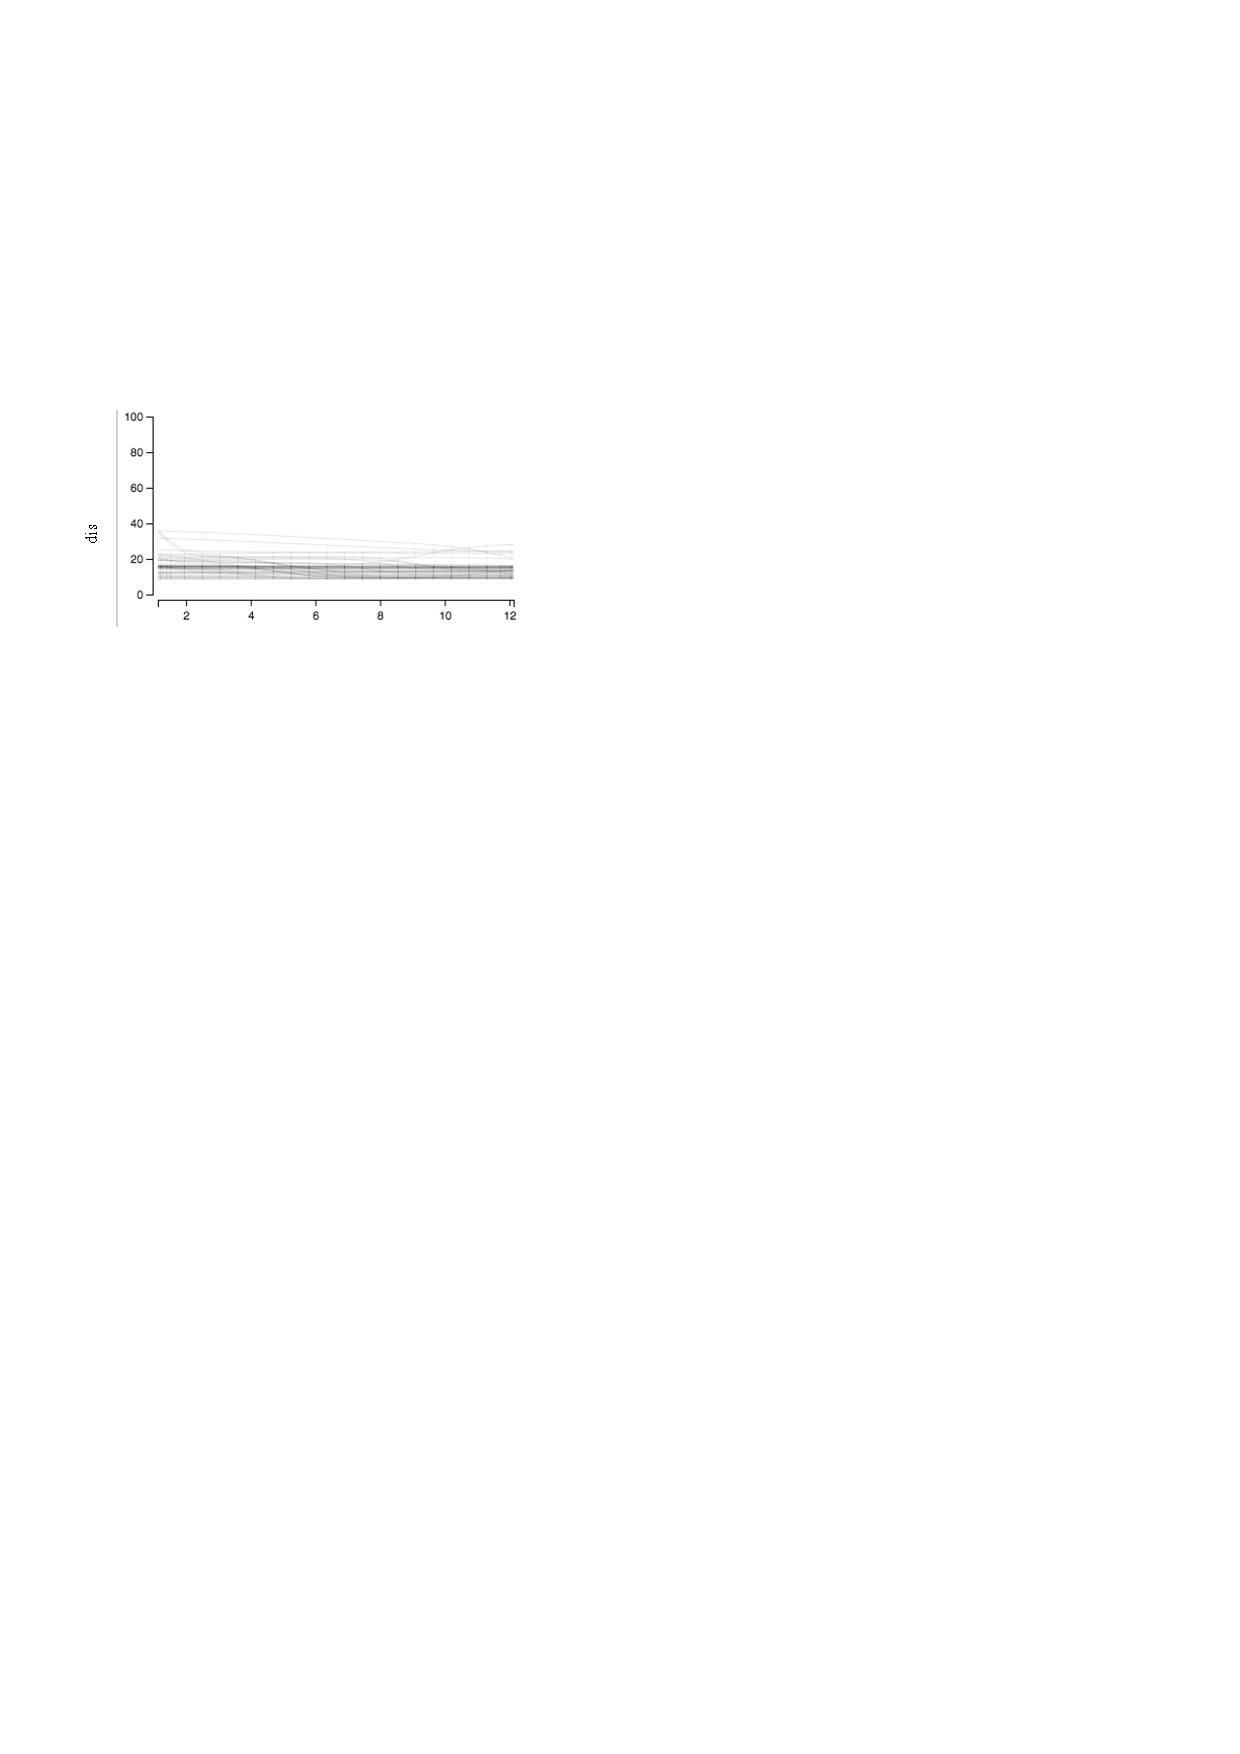
\includegraphics[width=\textwidth]{nn5x3_8.pdf}
    \end{subfigure}
    &
    \begin{subfigure}[b]{0.2\textwidth}
      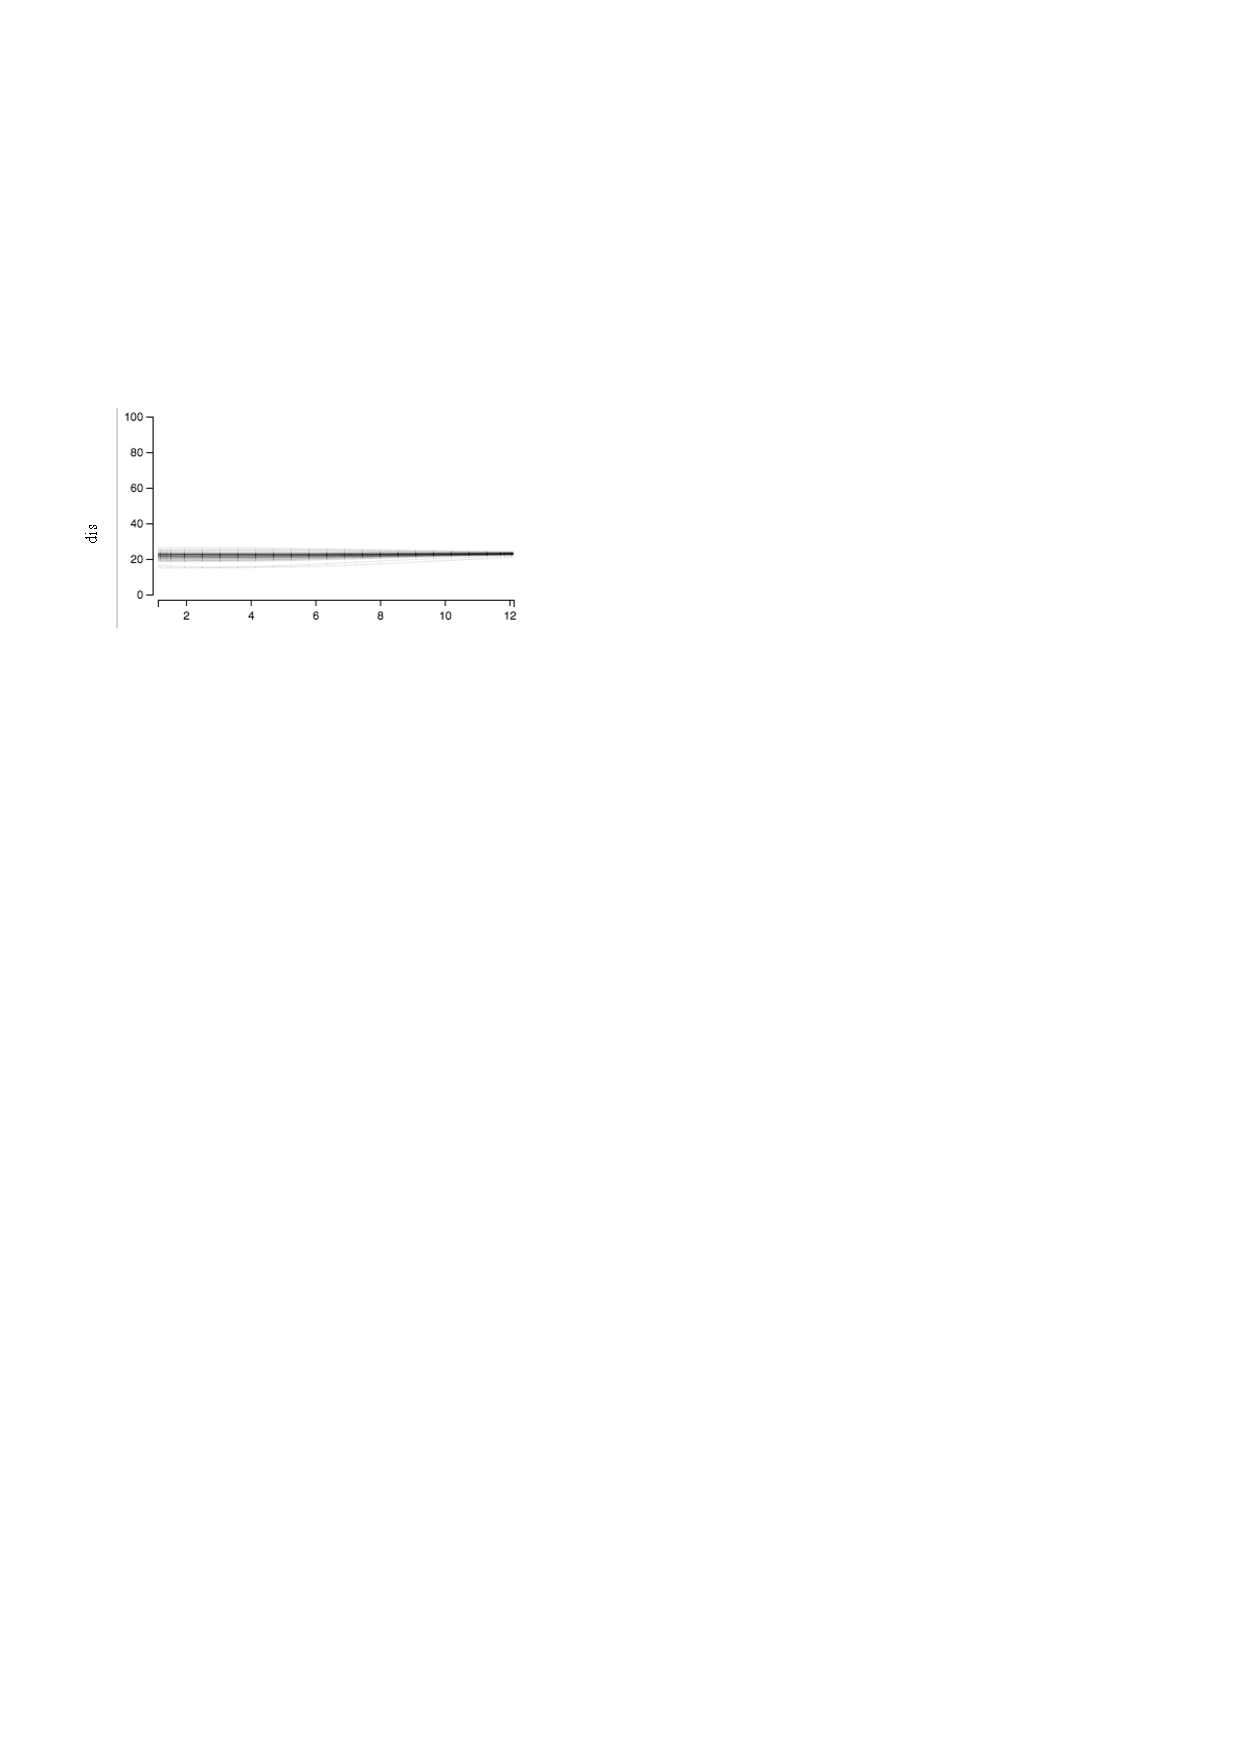
\includegraphics[width=\textwidth]{svmr_8.pdf}
    \end{subfigure}
    \\
    \hline \\
    Accessibility to radial highways &
    \begin{subfigure}[b]{0.2\textwidth}
      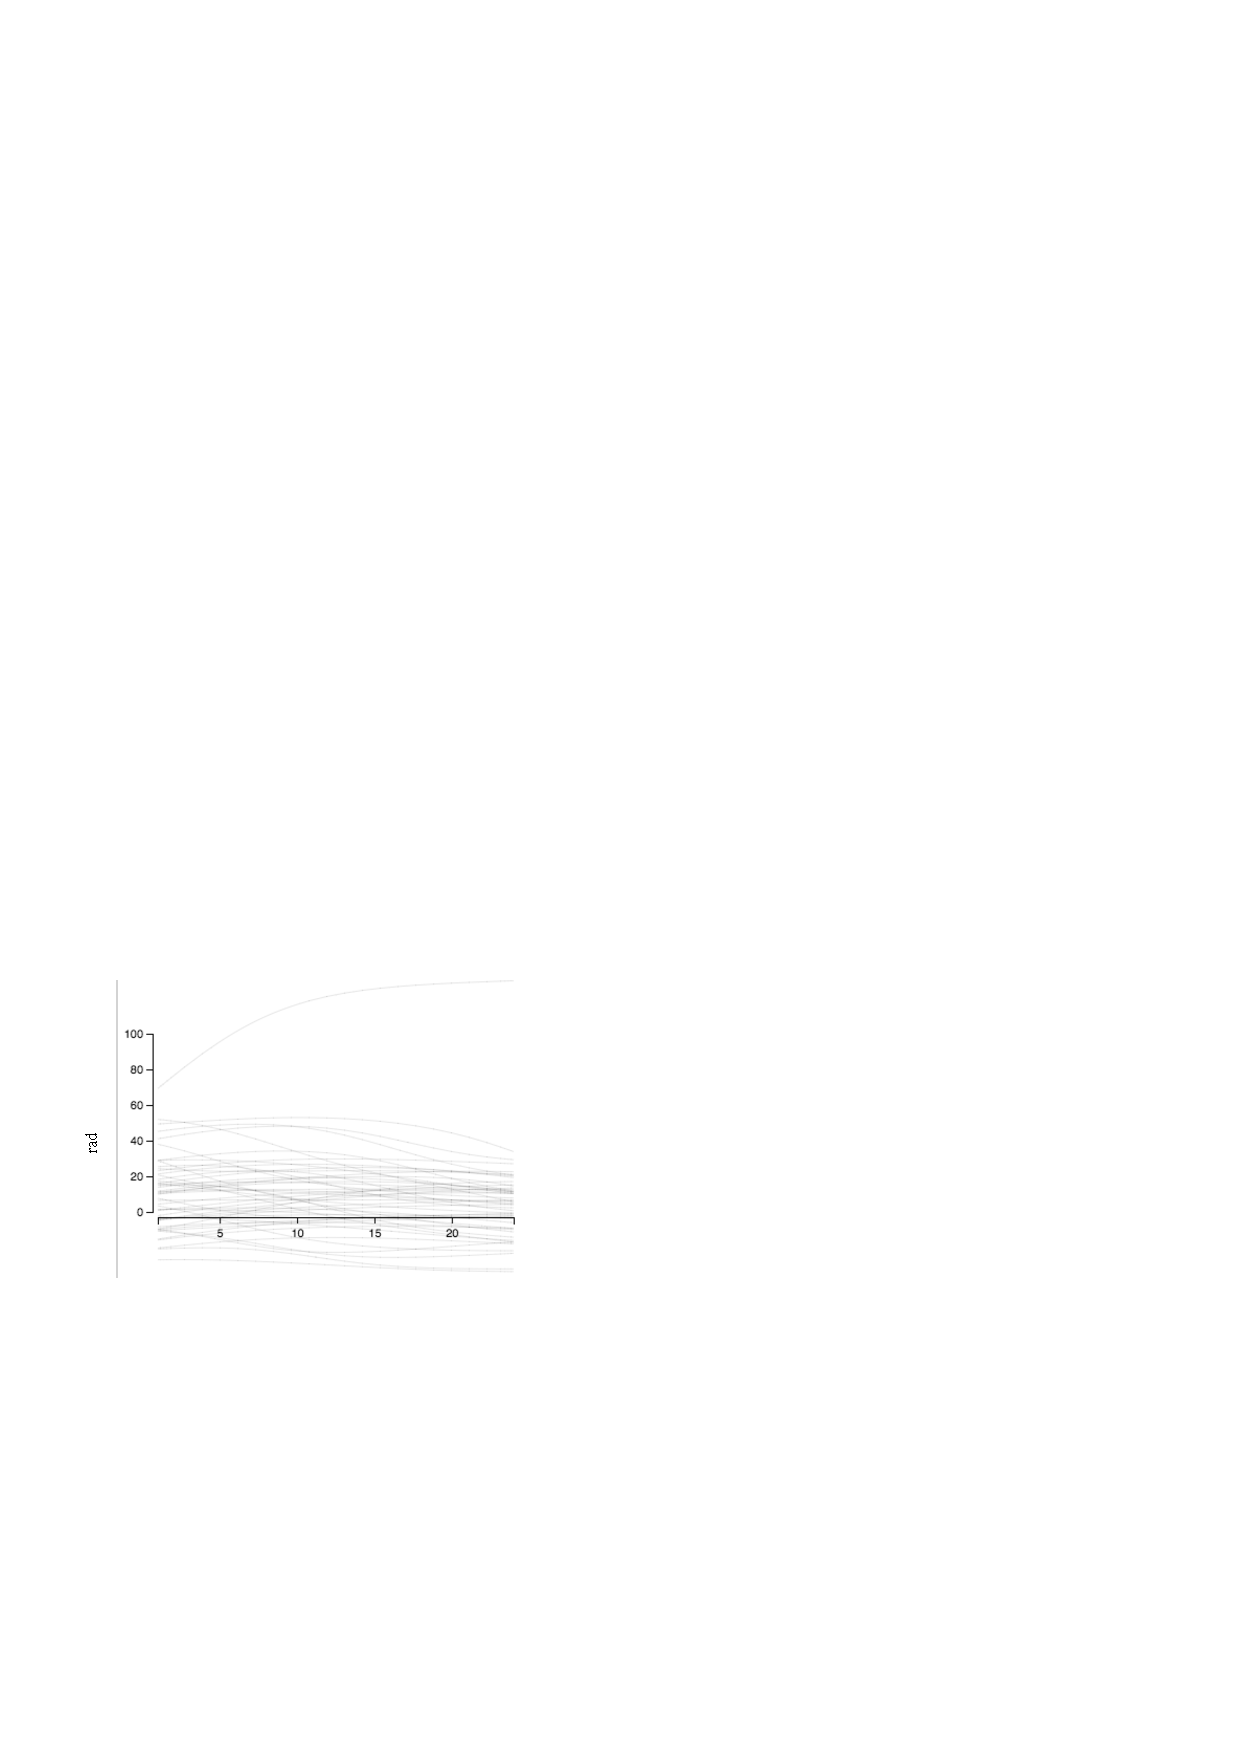
\includegraphics[width=\textwidth]{nn26_9.pdf}
    \end{subfigure}
    &
    \begin{subfigure}[b]{0.2\textwidth}
      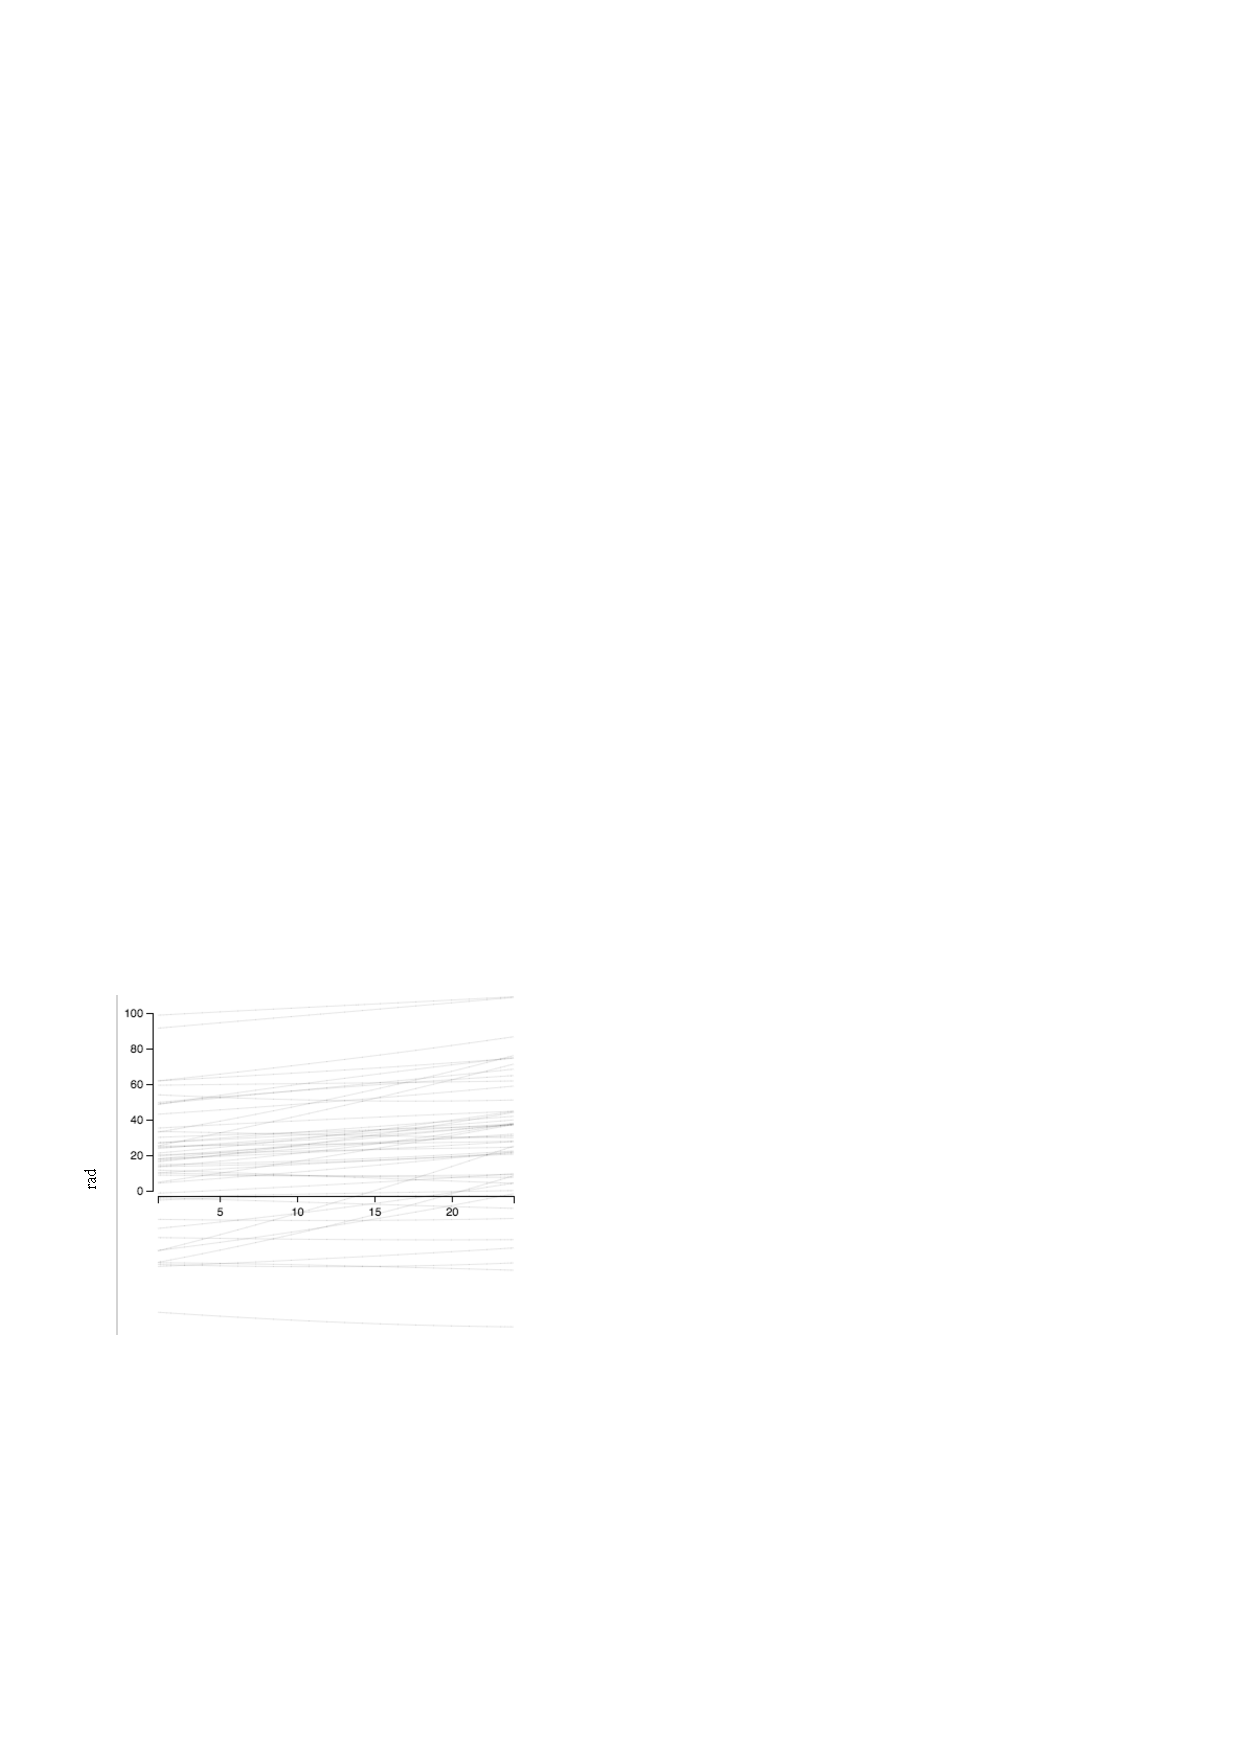
\includegraphics[width=\textwidth]{svmp_9.pdf}
    \end{subfigure}
    &
    \begin{subfigure}[b]{0.2\textwidth}
      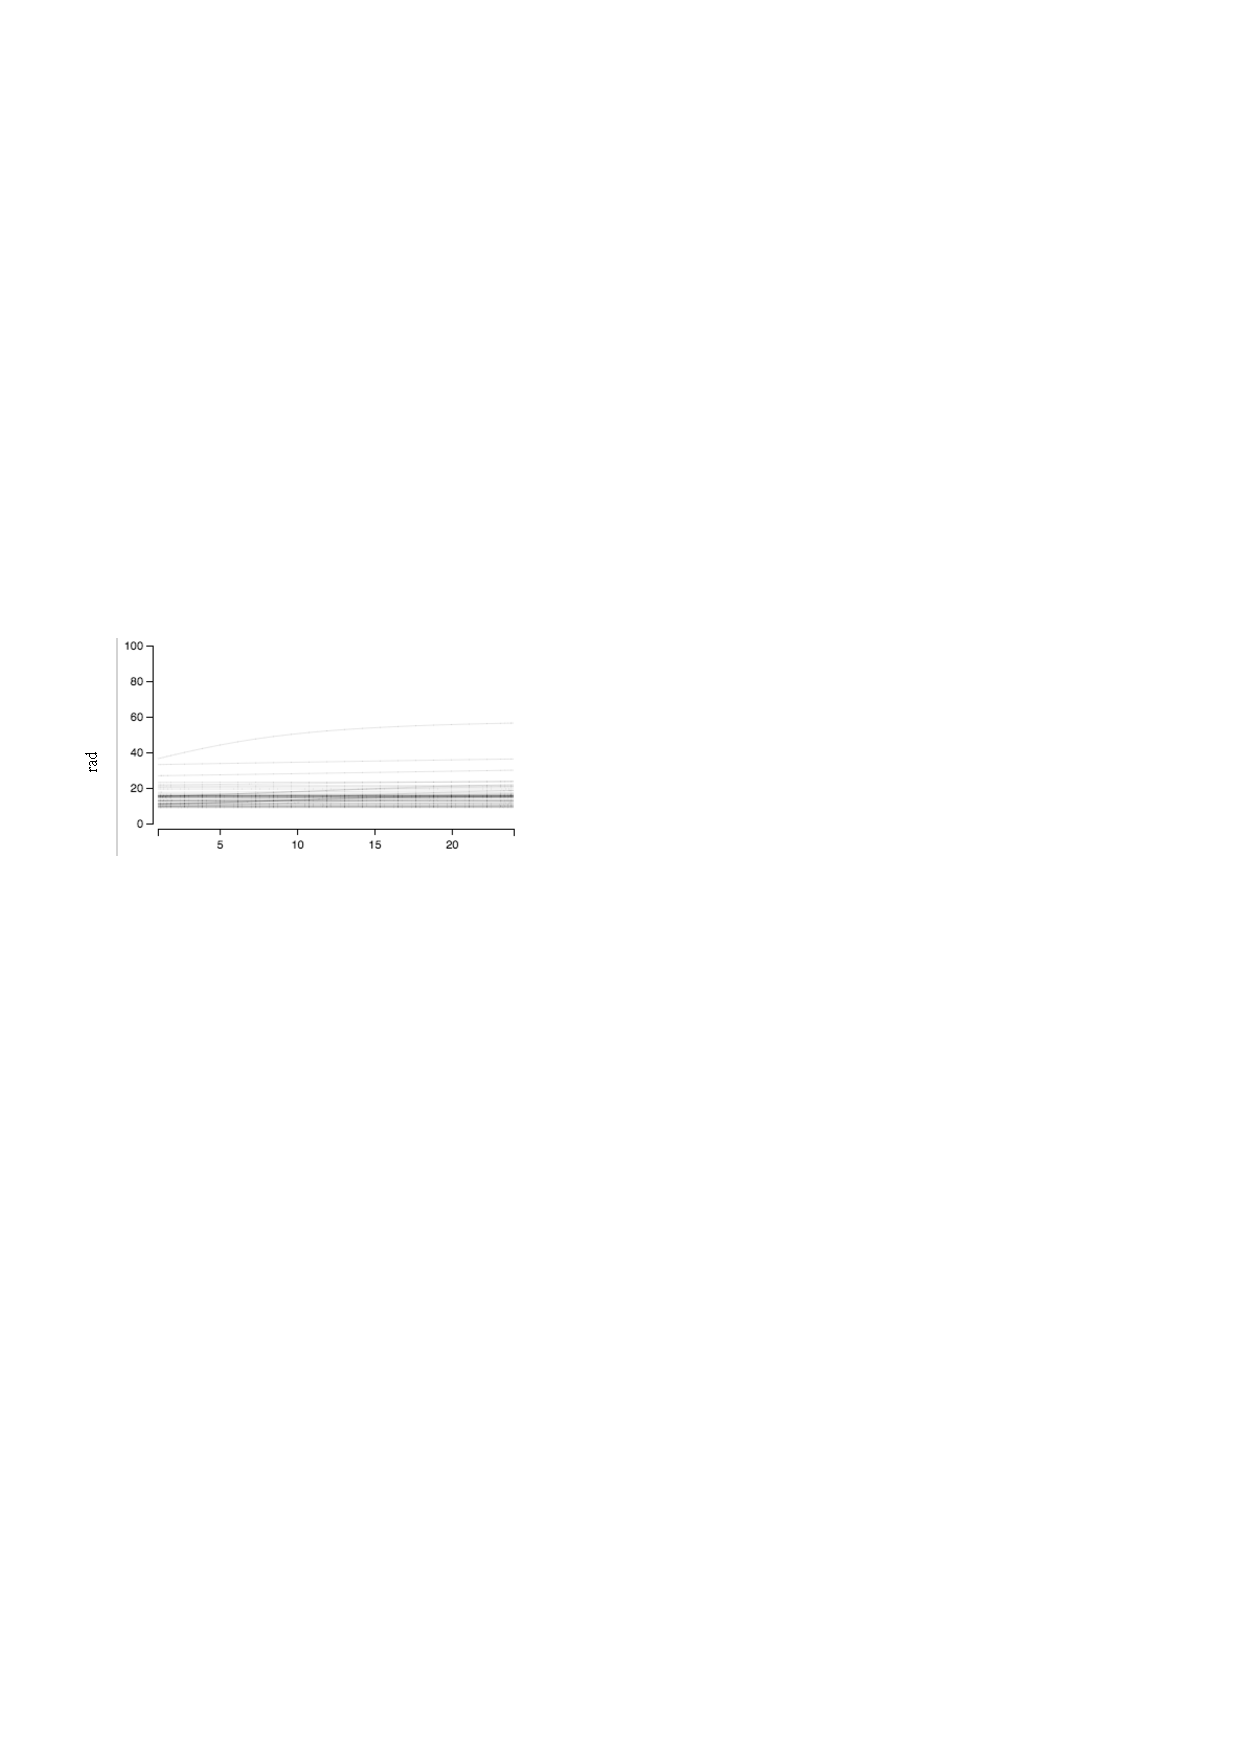
\includegraphics[width=\textwidth]{nn5x3_9.pdf}
    \end{subfigure}
    &
    \begin{subfigure}[b]{0.2\textwidth}
      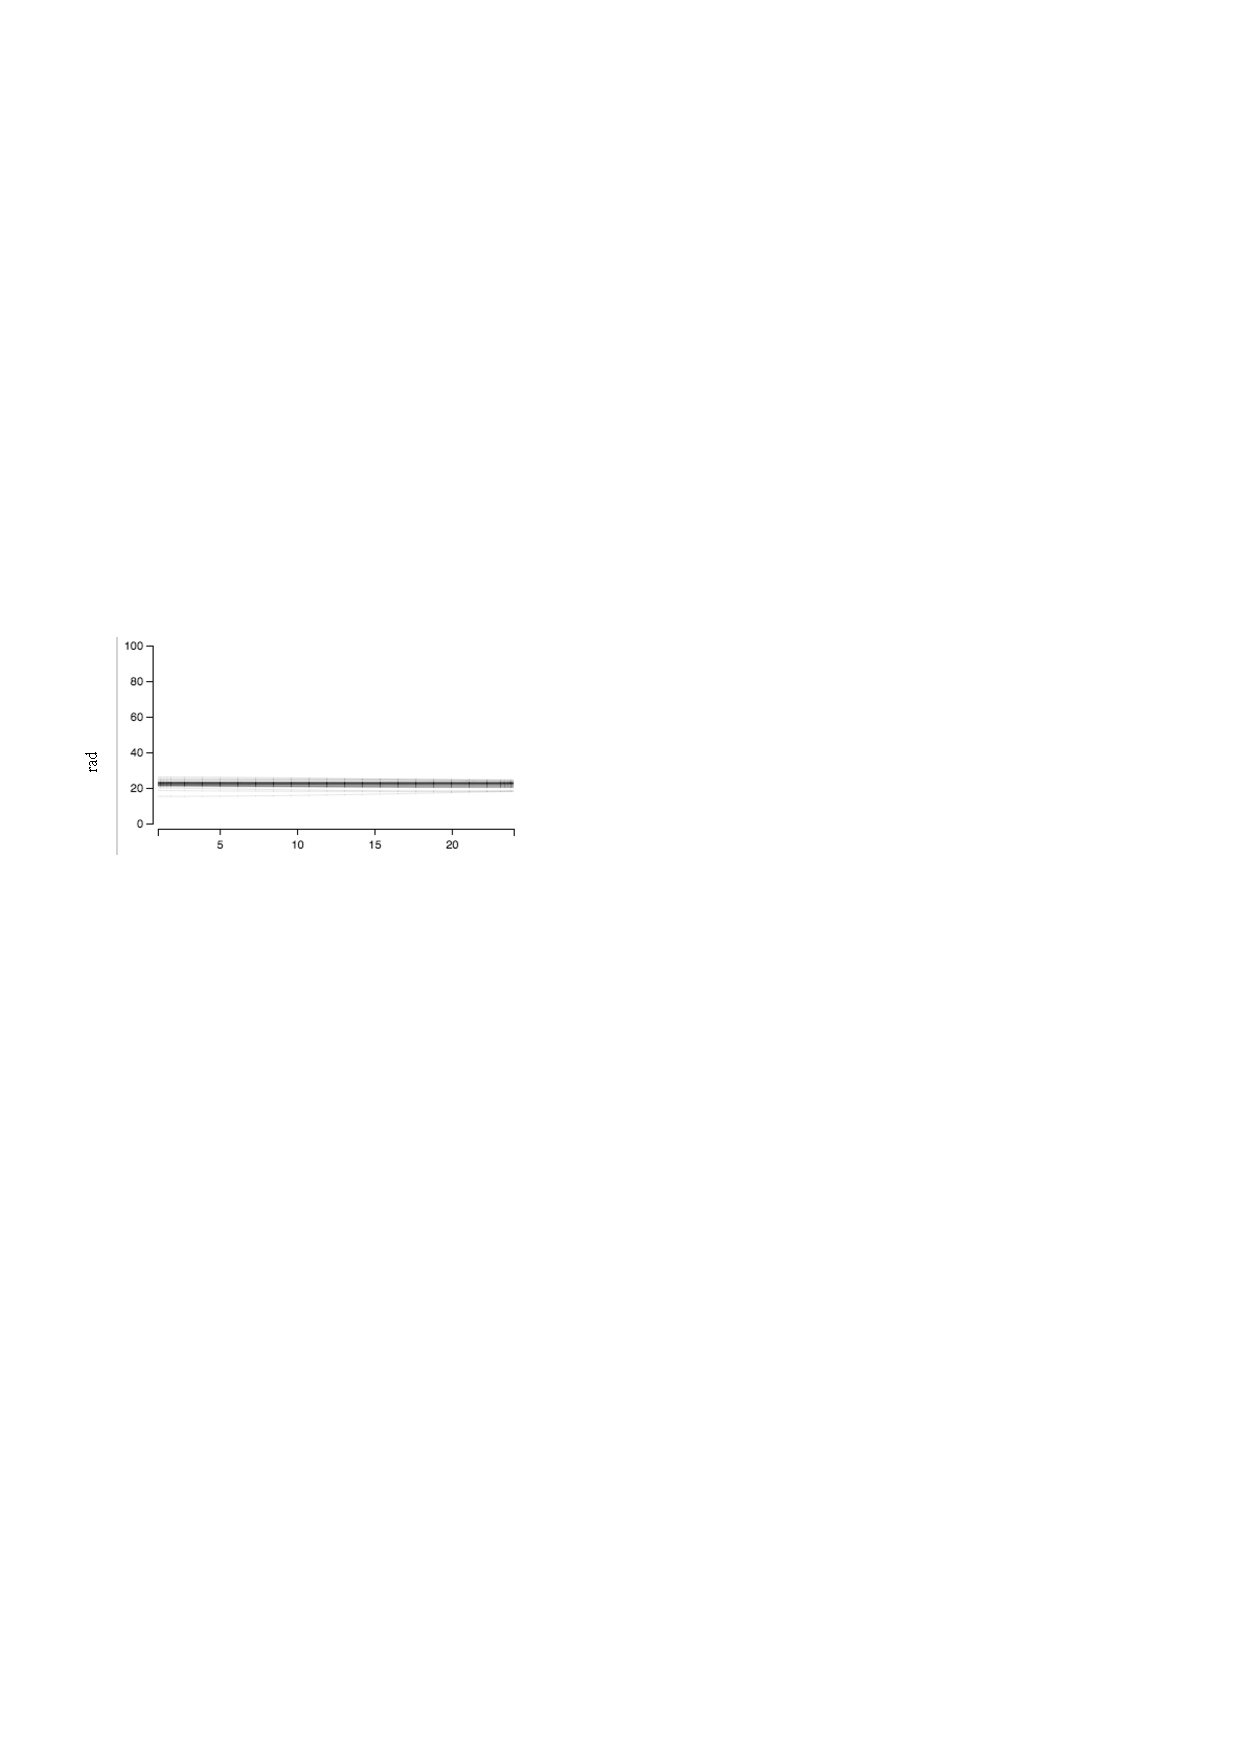
\includegraphics[width=\textwidth]{svmr_9.pdf}
    \end{subfigure}
    \\
    \hline \\
    Property-tax rate &
    \begin{subfigure}[b]{0.2\textwidth}
      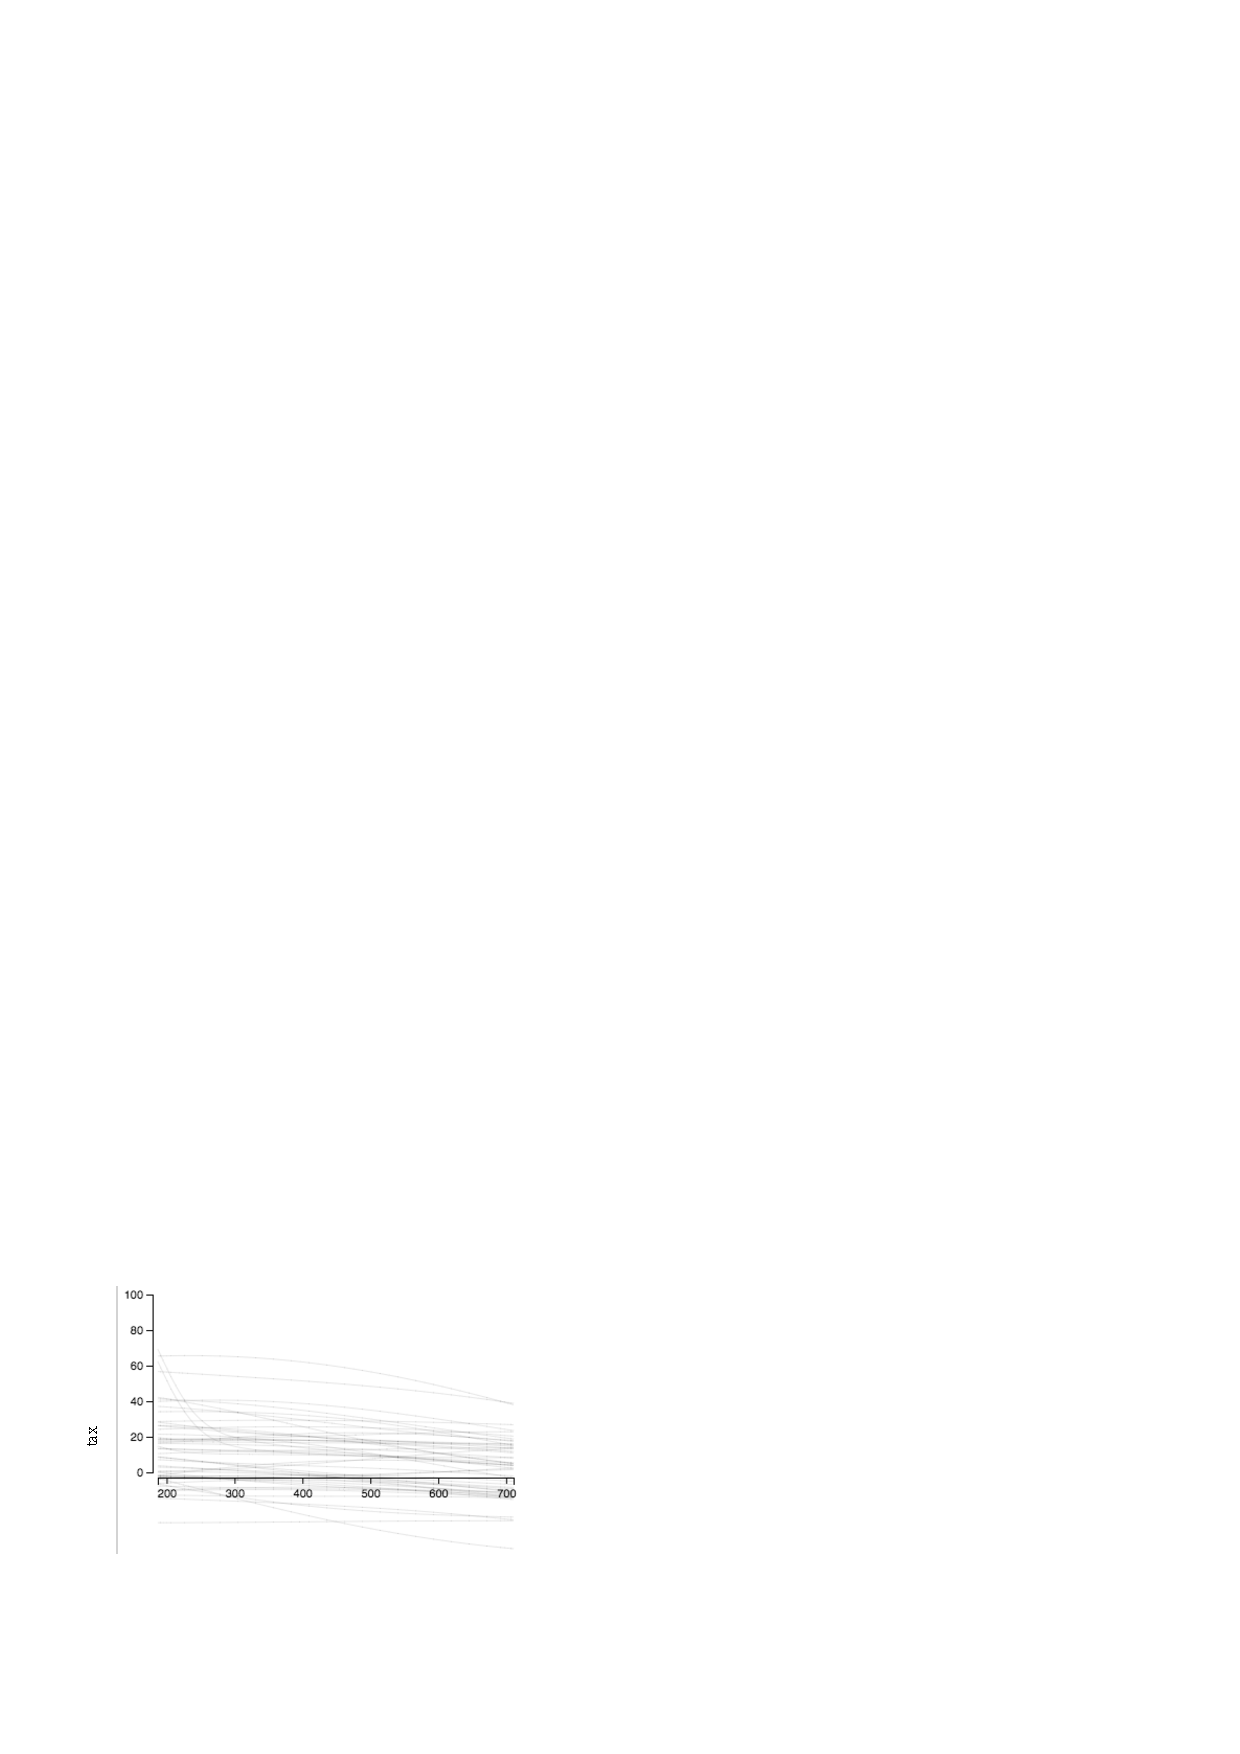
\includegraphics[width=\textwidth]{nn26_10.pdf}
    \end{subfigure}
    &
    \begin{subfigure}[b]{0.2\textwidth}
      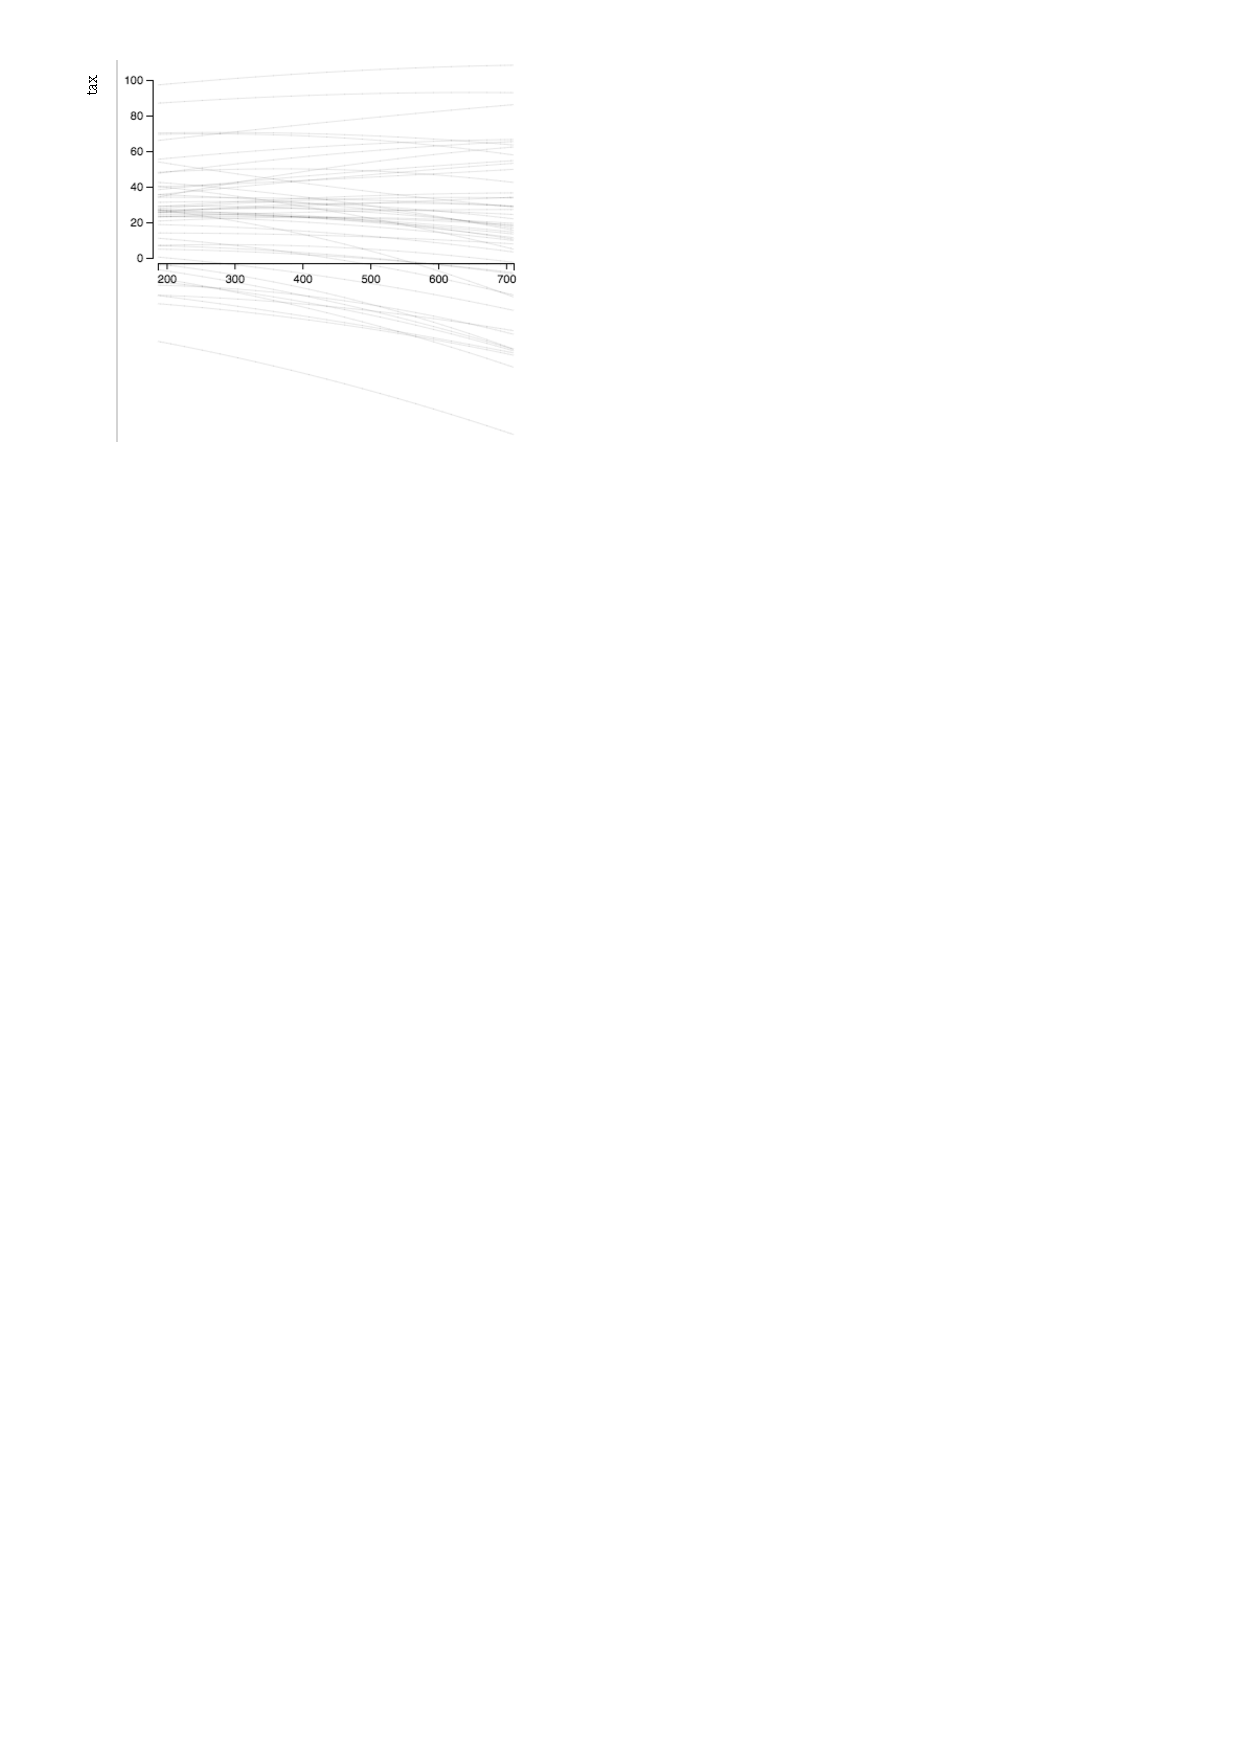
\includegraphics[width=\textwidth]{svmp_10.pdf}
    \end{subfigure}
    &
    \begin{subfigure}[b]{0.2\textwidth}
      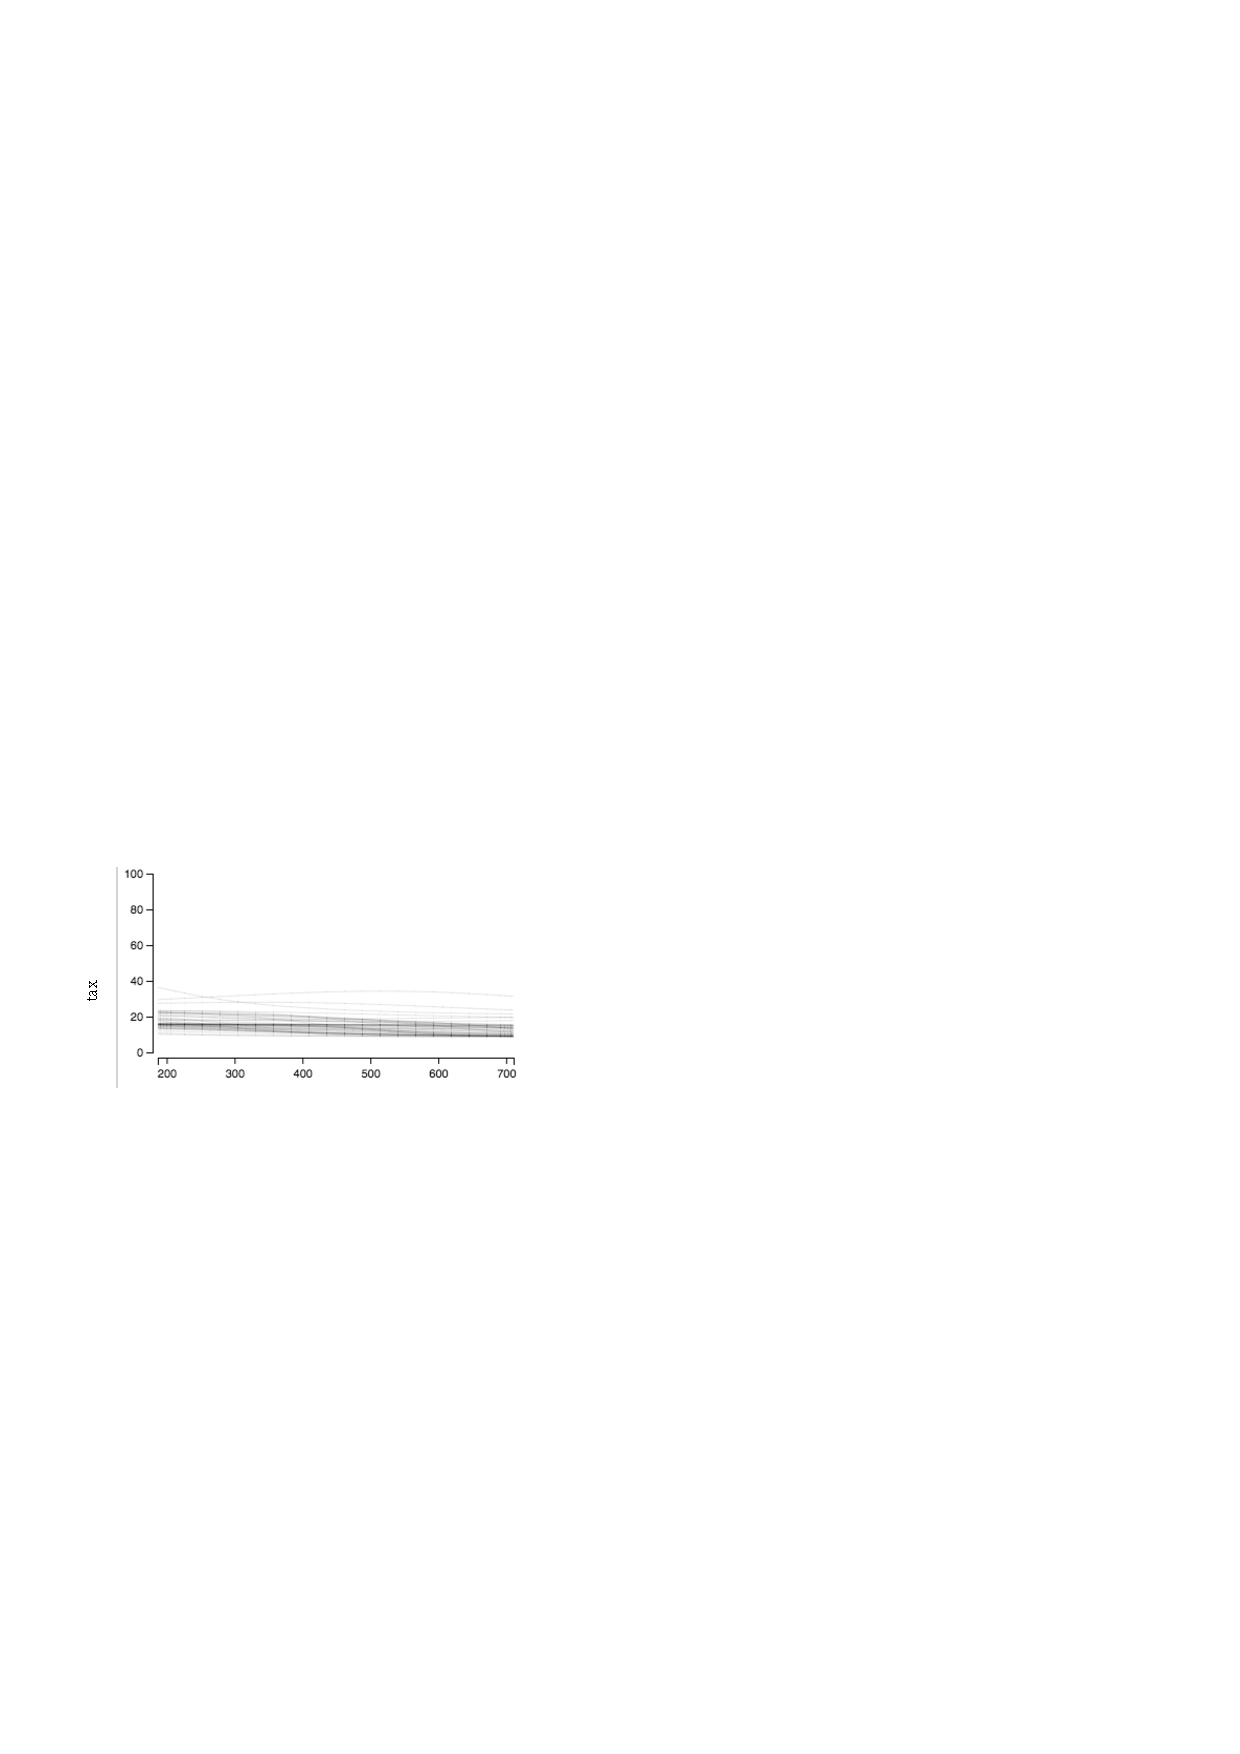
\includegraphics[width=\textwidth]{nn5x3_10.pdf}
    \end{subfigure}
    &
    \begin{subfigure}[b]{0.2\textwidth}
      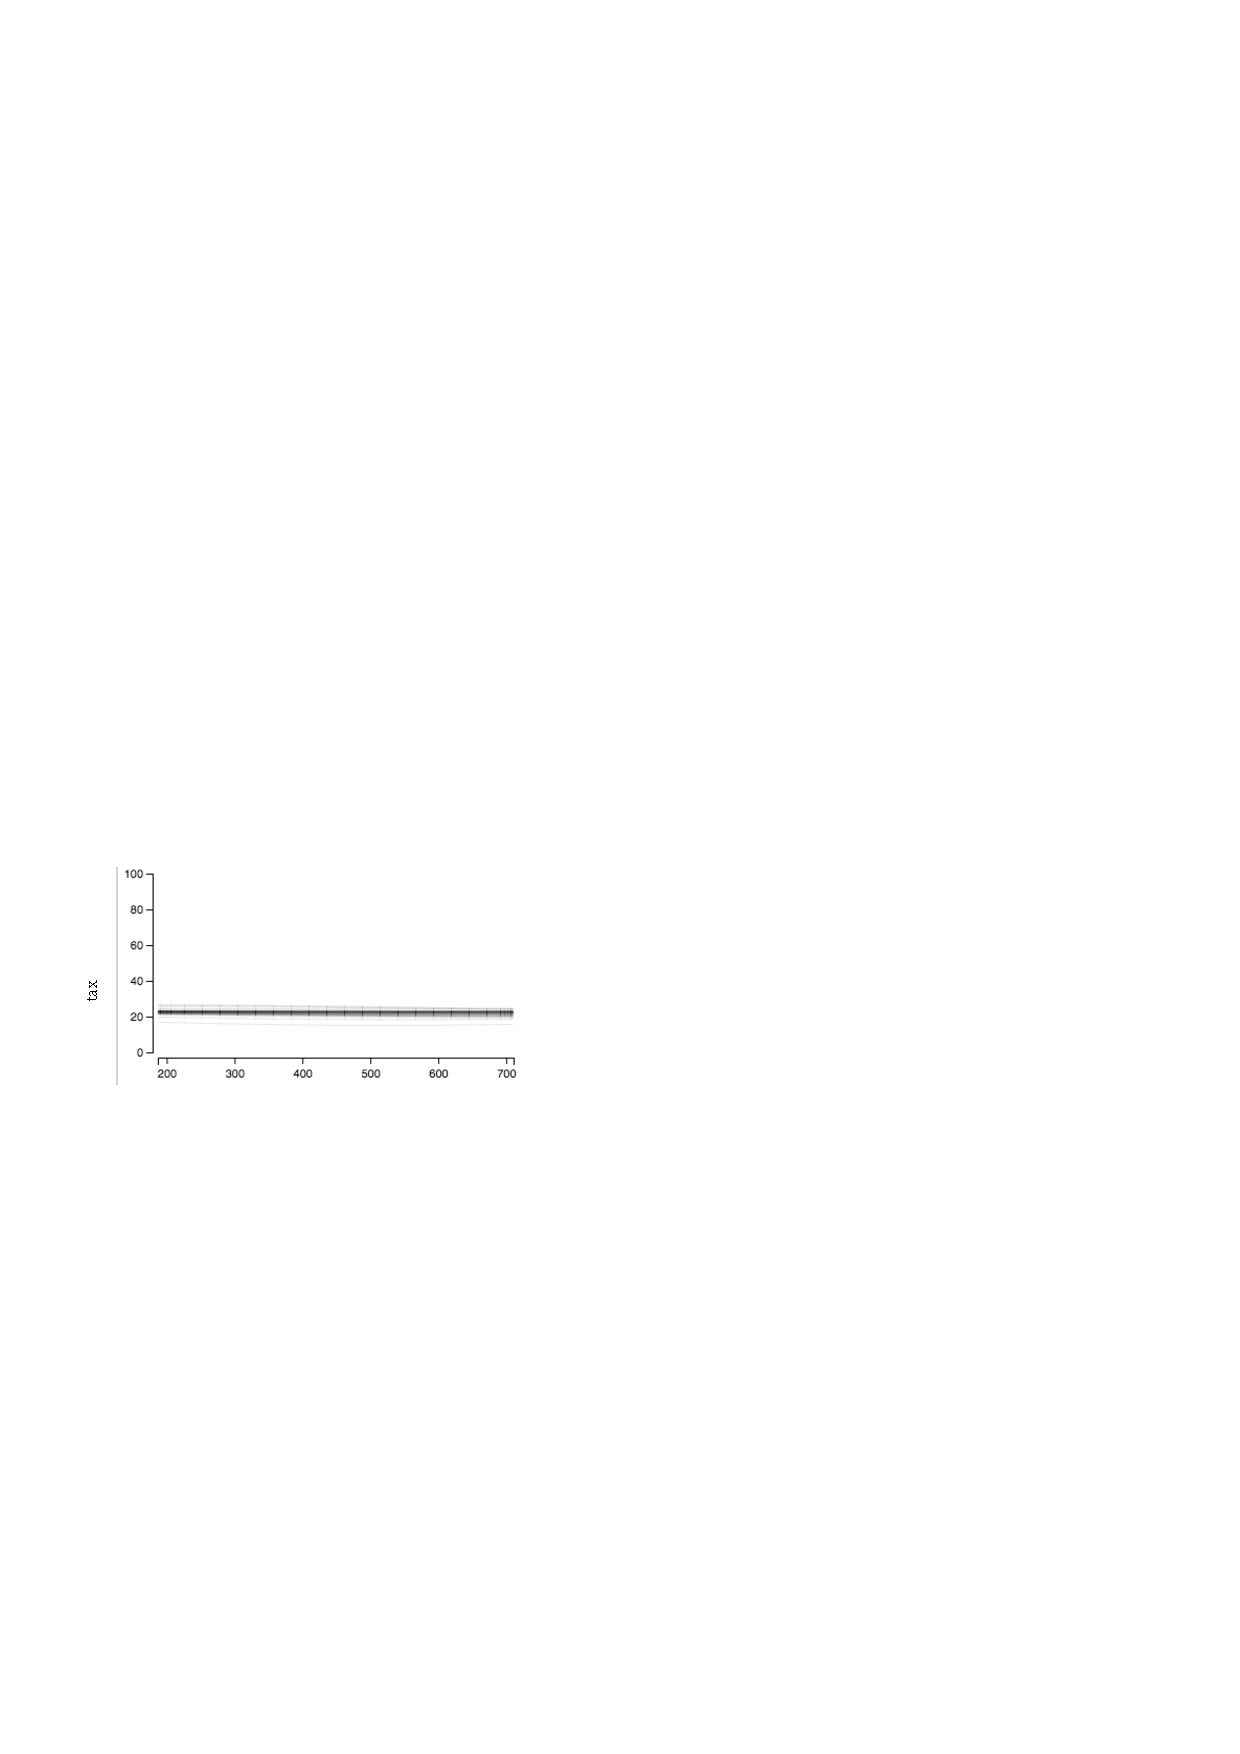
\includegraphics[width=\textwidth]{svmr_10.pdf}
    \end{subfigure}
    \\
    \hline \\
    Pupil-teacher ratio &
    \begin{subfigure}[b]{0.2\textwidth}
      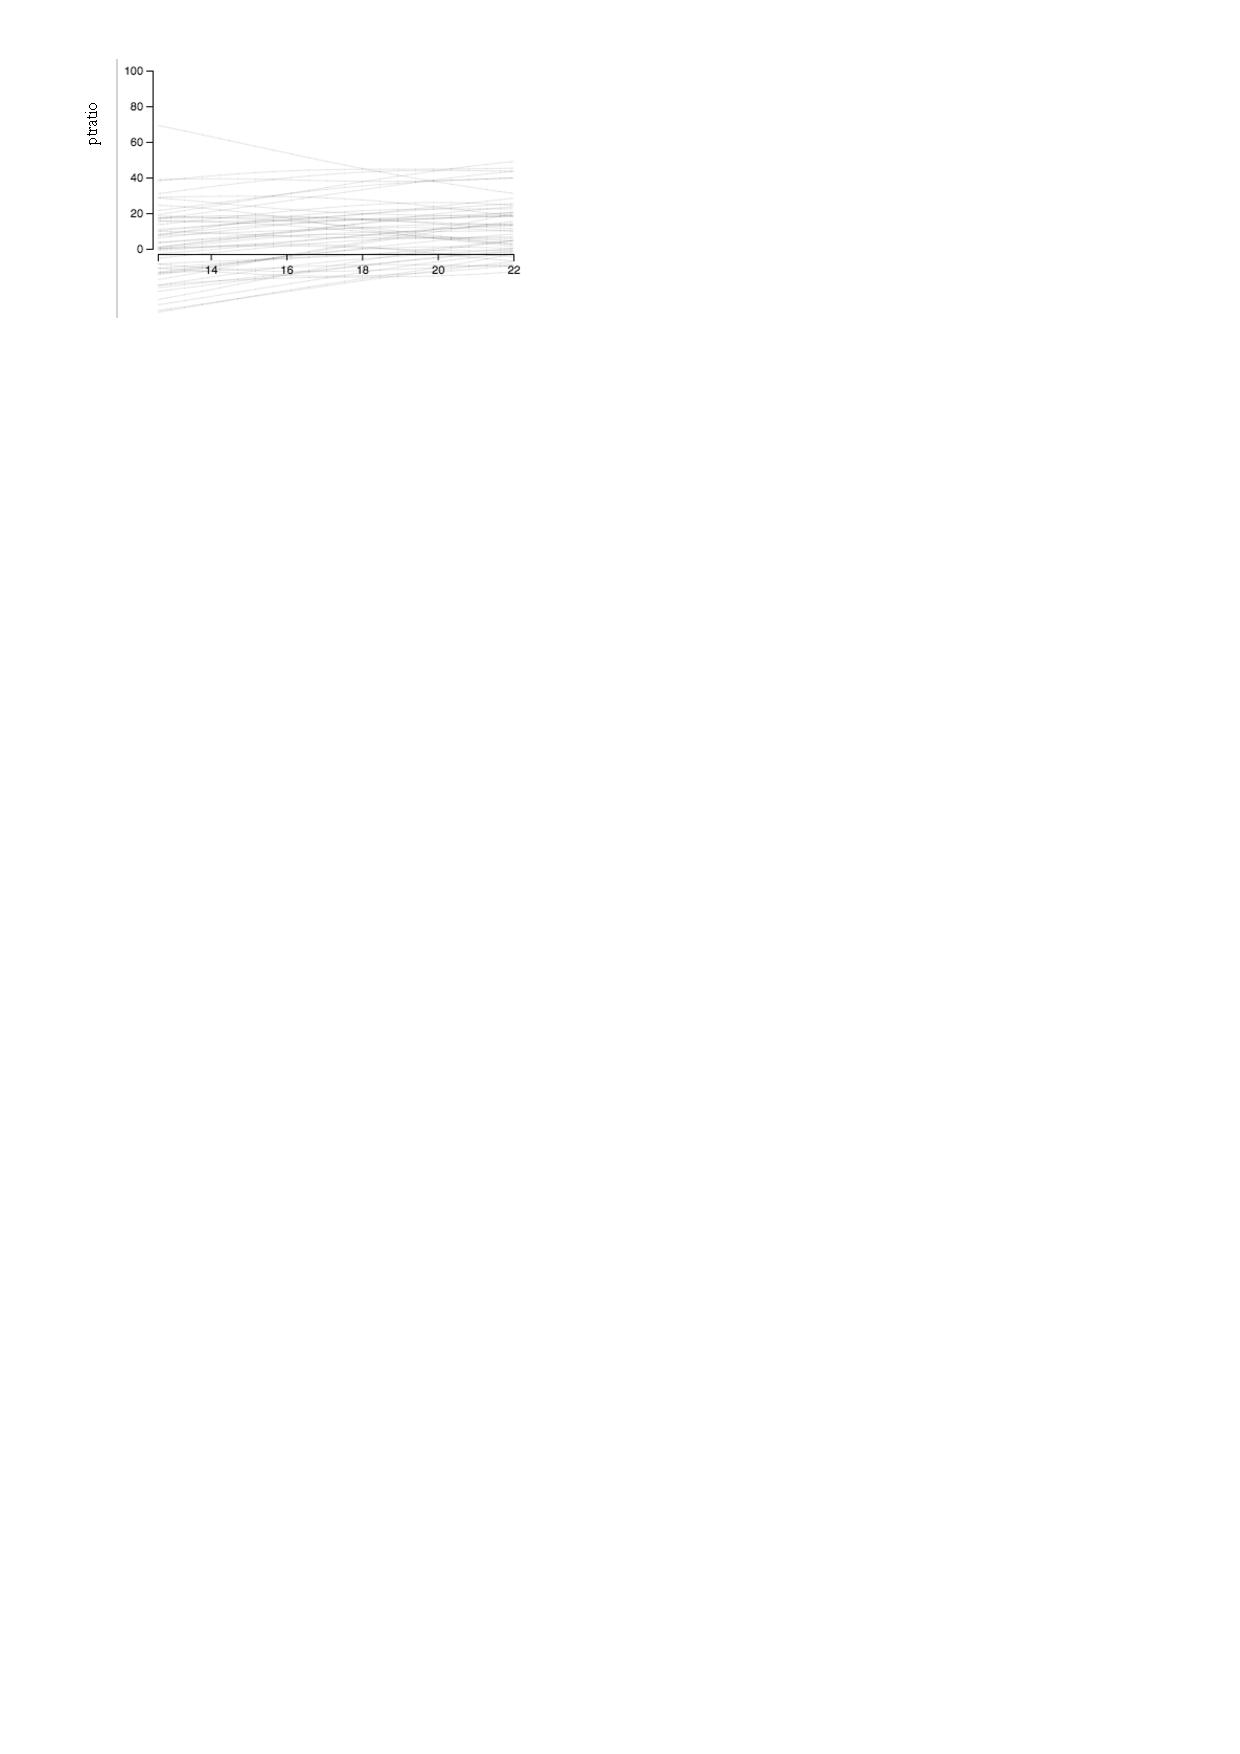
\includegraphics[width=\textwidth]{nn26_11.pdf}
    \end{subfigure}
    &
    \begin{subfigure}[b]{0.2\textwidth}
      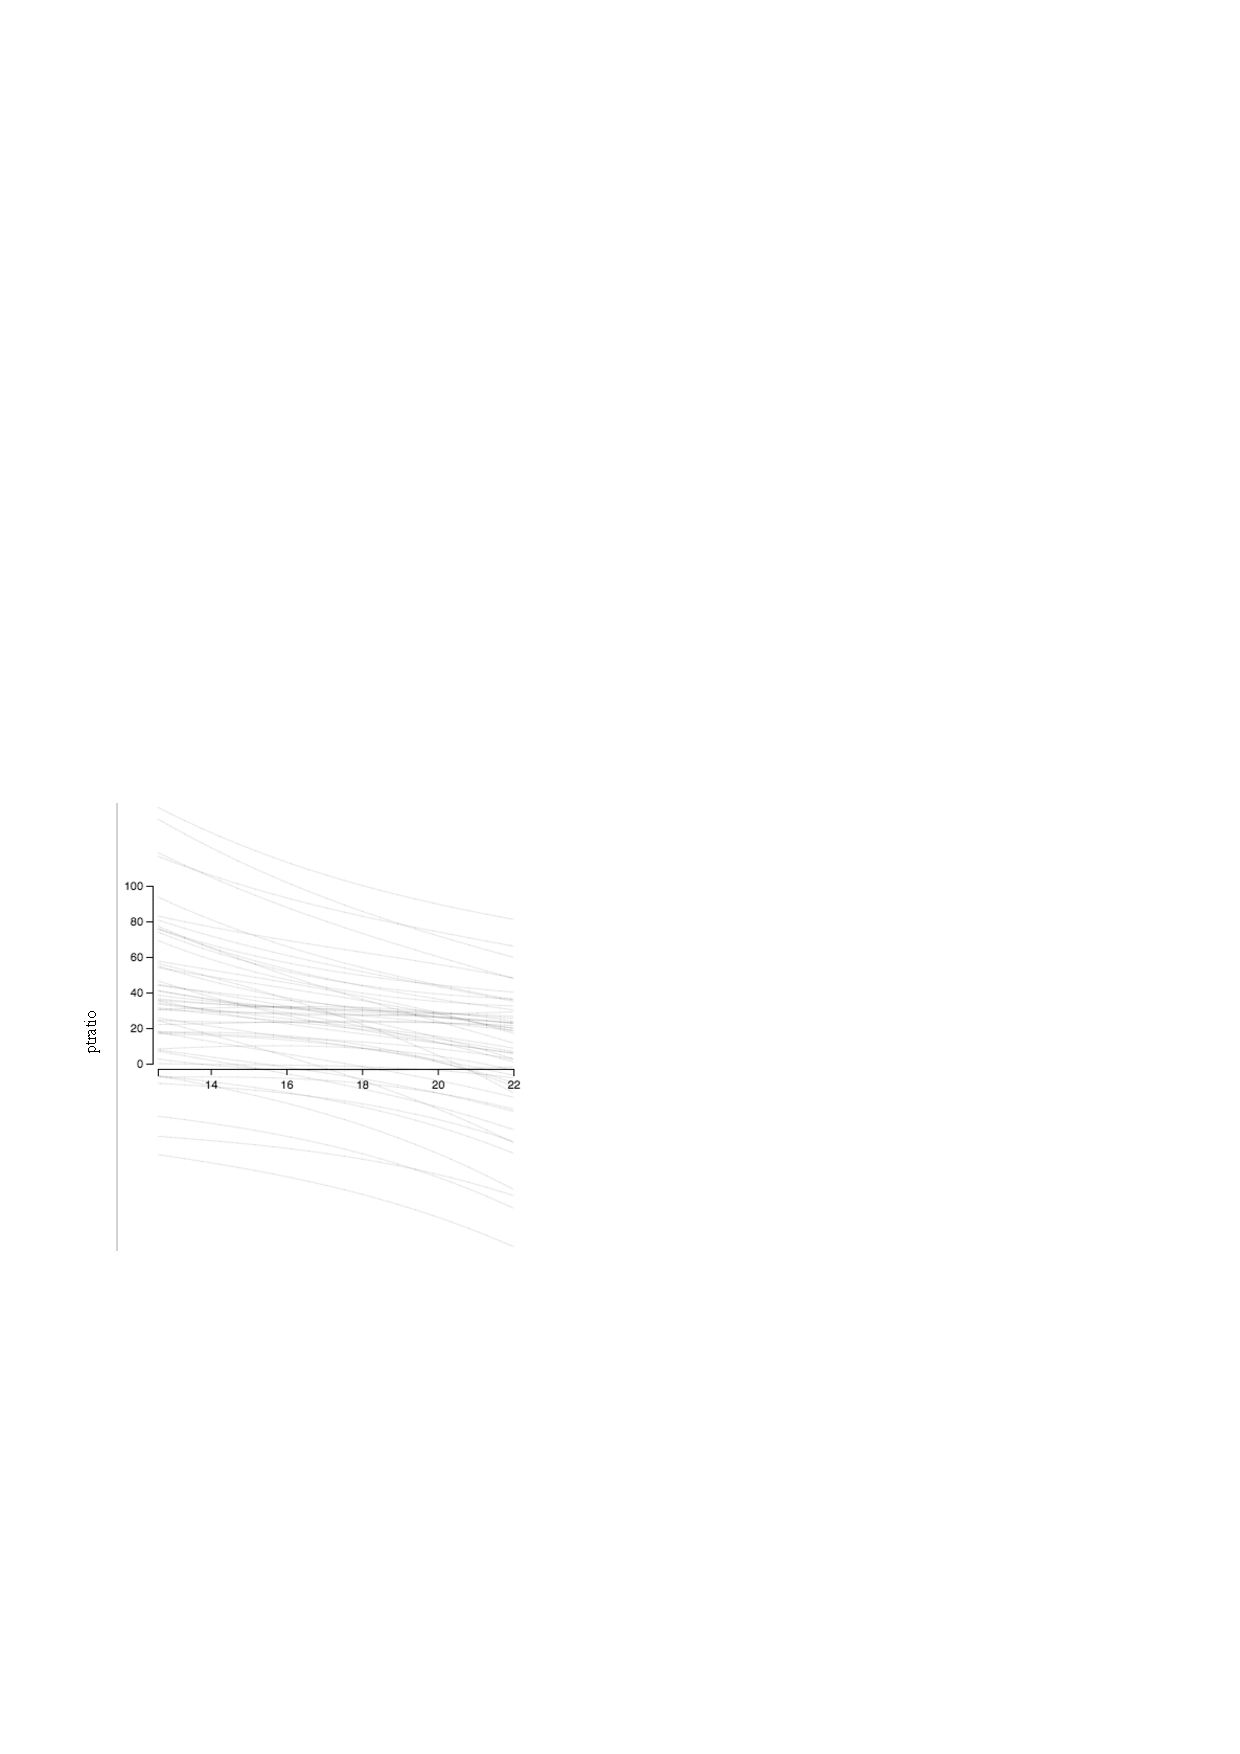
\includegraphics[width=\textwidth]{svmp_11.pdf}
    \end{subfigure}
    &
    \begin{subfigure}[b]{0.2\textwidth}
      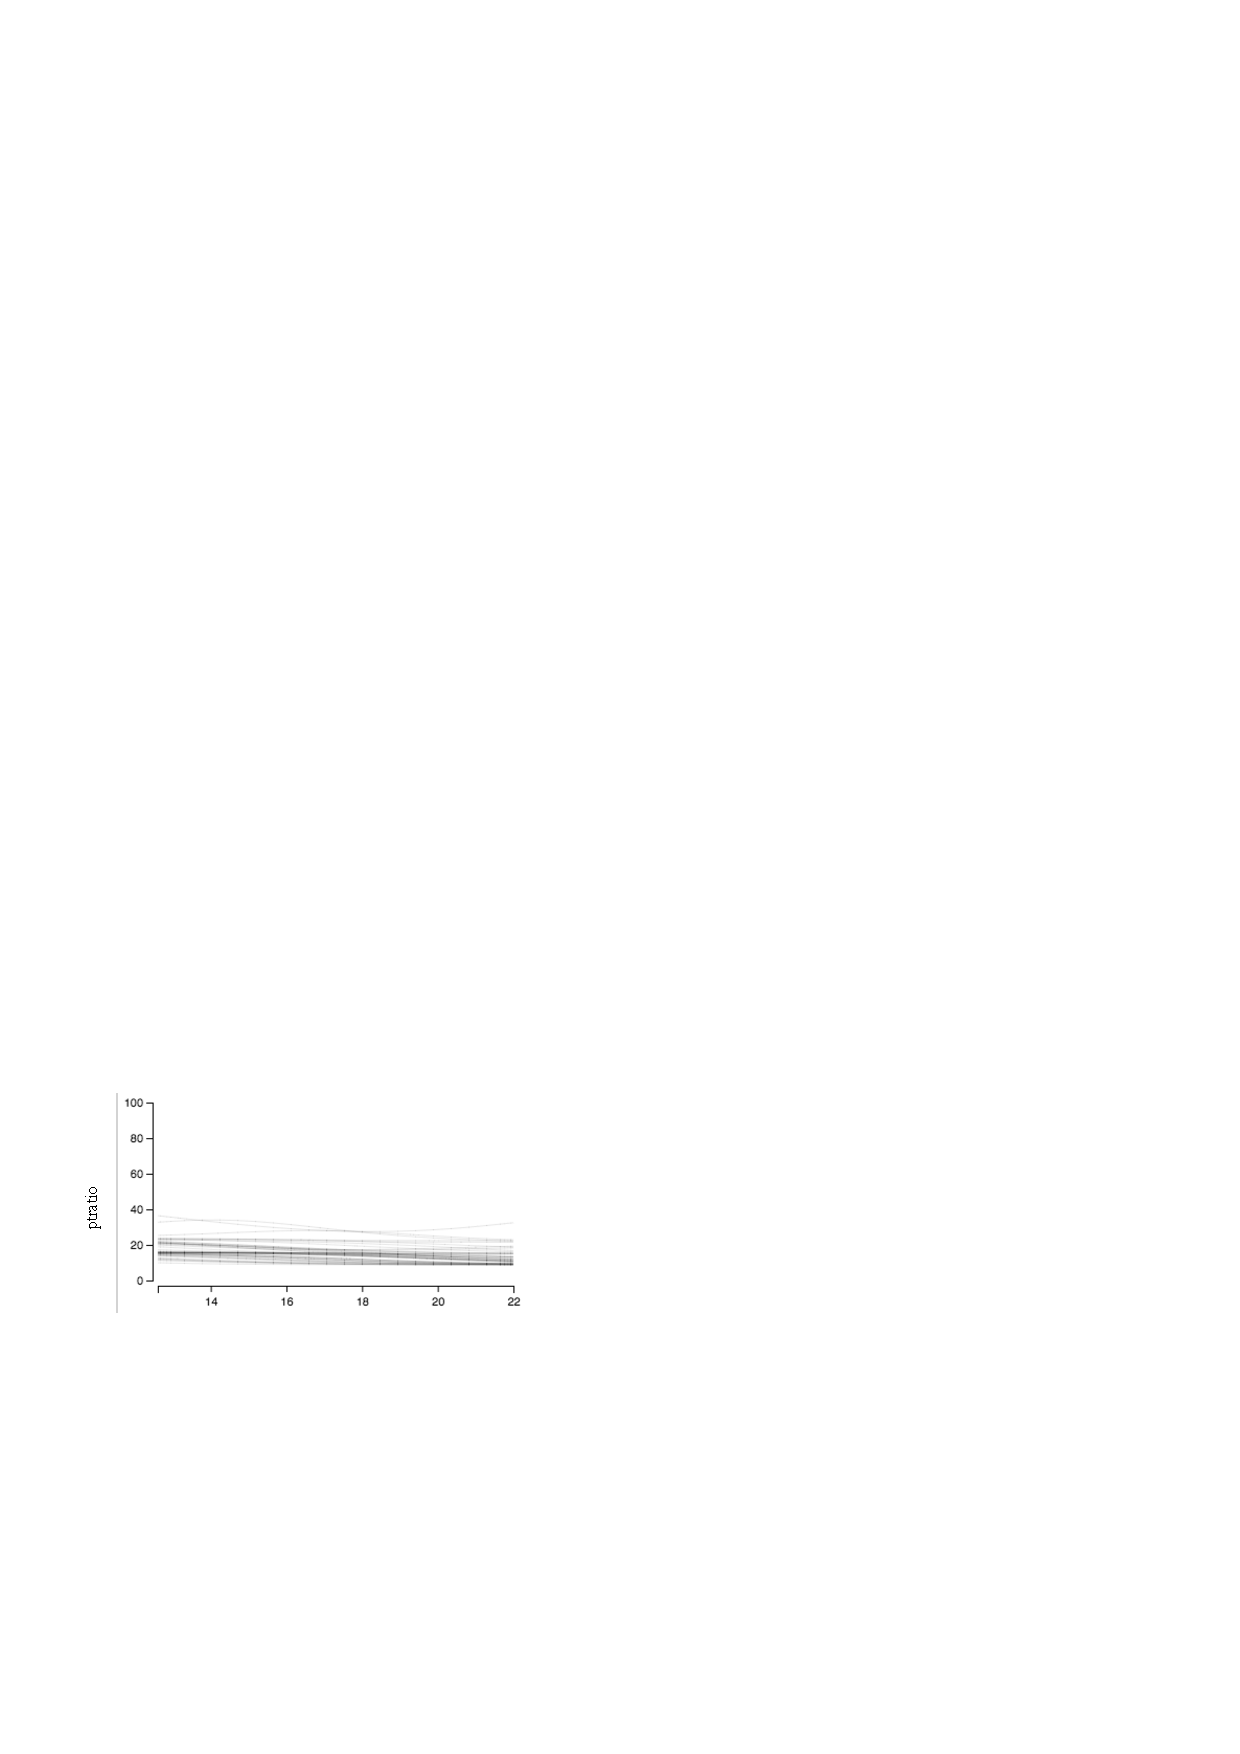
\includegraphics[width=\textwidth]{nn5x3_11.pdf}
    \end{subfigure}
    &
    \begin{subfigure}[b]{0.2\textwidth}
      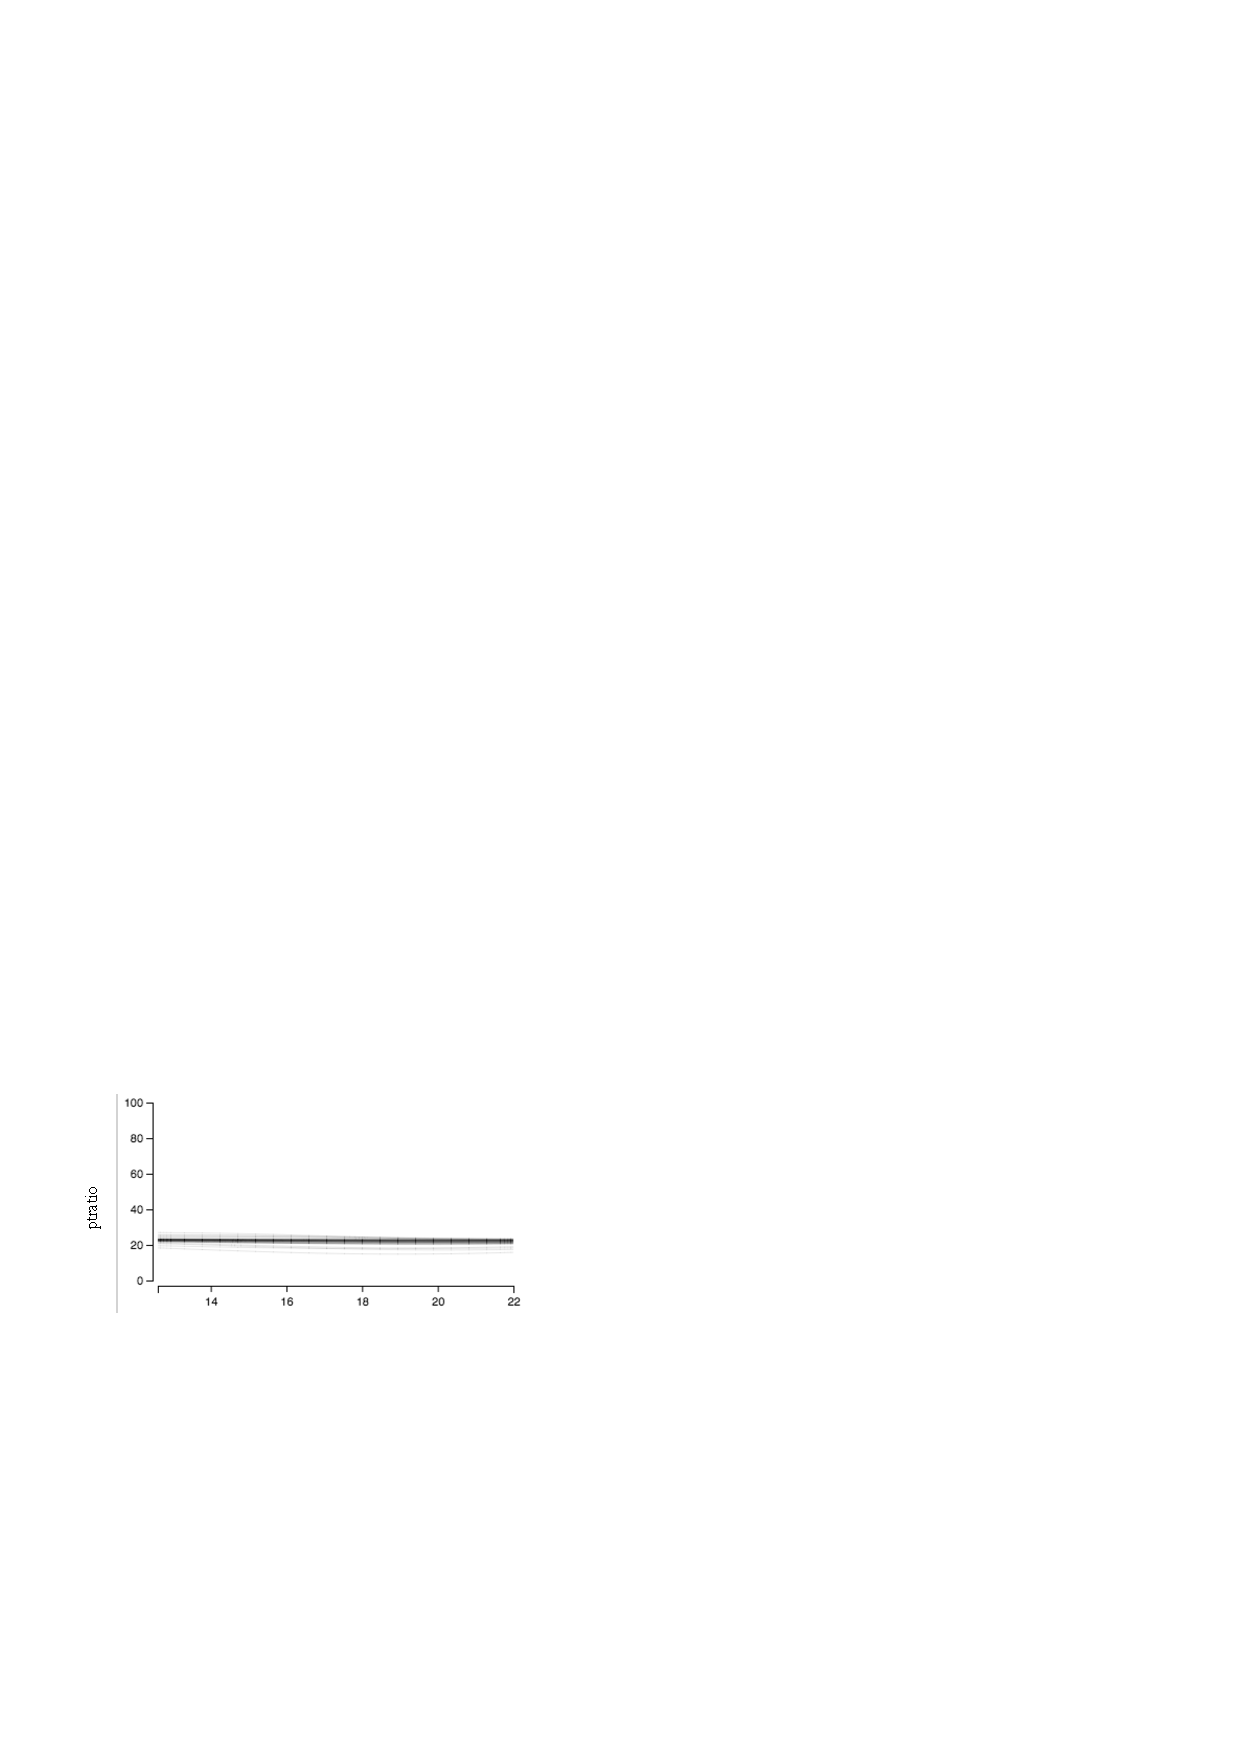
\includegraphics[width=\textwidth]{svmr_11.pdf}
    \end{subfigure}
    \\
    \hline \\
    Proportion of blacks &
    \begin{subfigure}[b]{0.2\textwidth}
      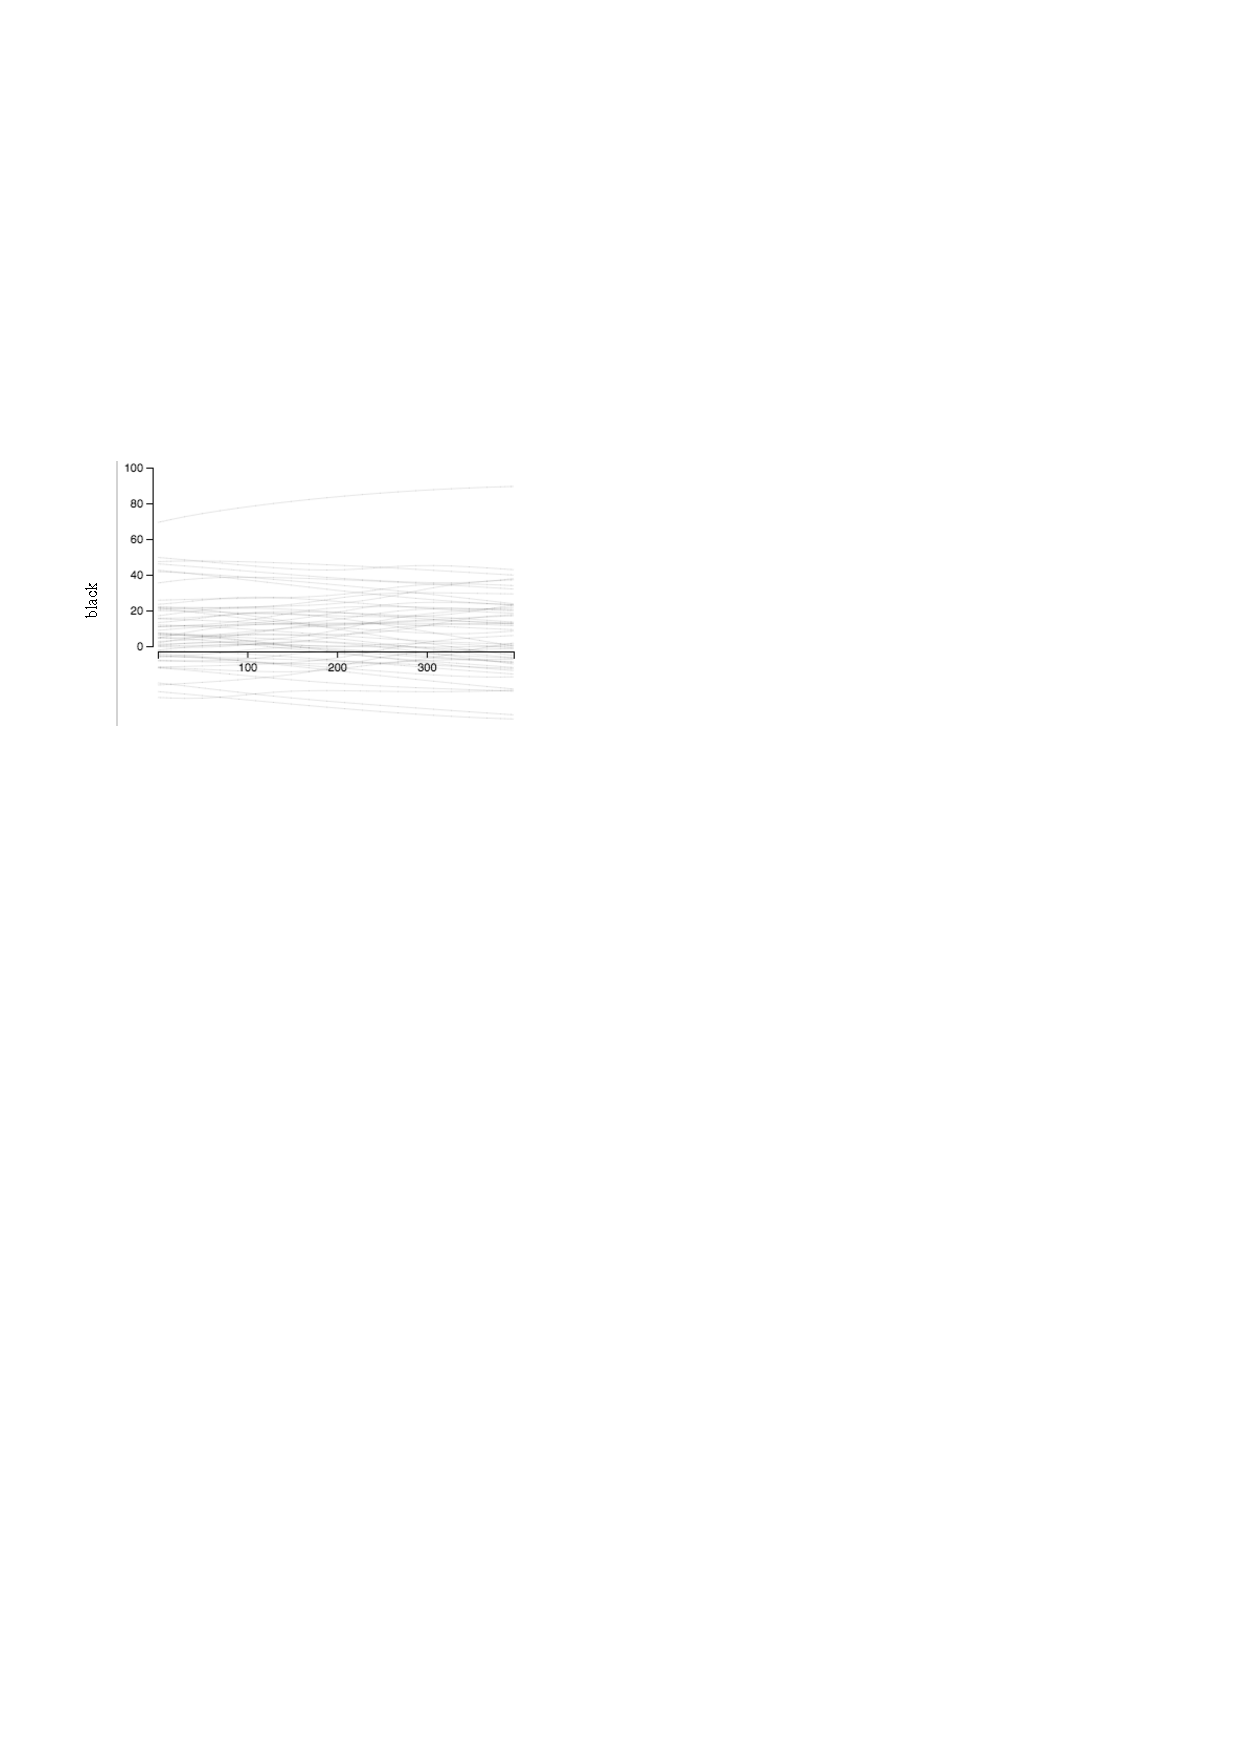
\includegraphics[width=\textwidth]{nn26_12.pdf}
    \end{subfigure}
    &
    \begin{subfigure}[b]{0.2\textwidth}
      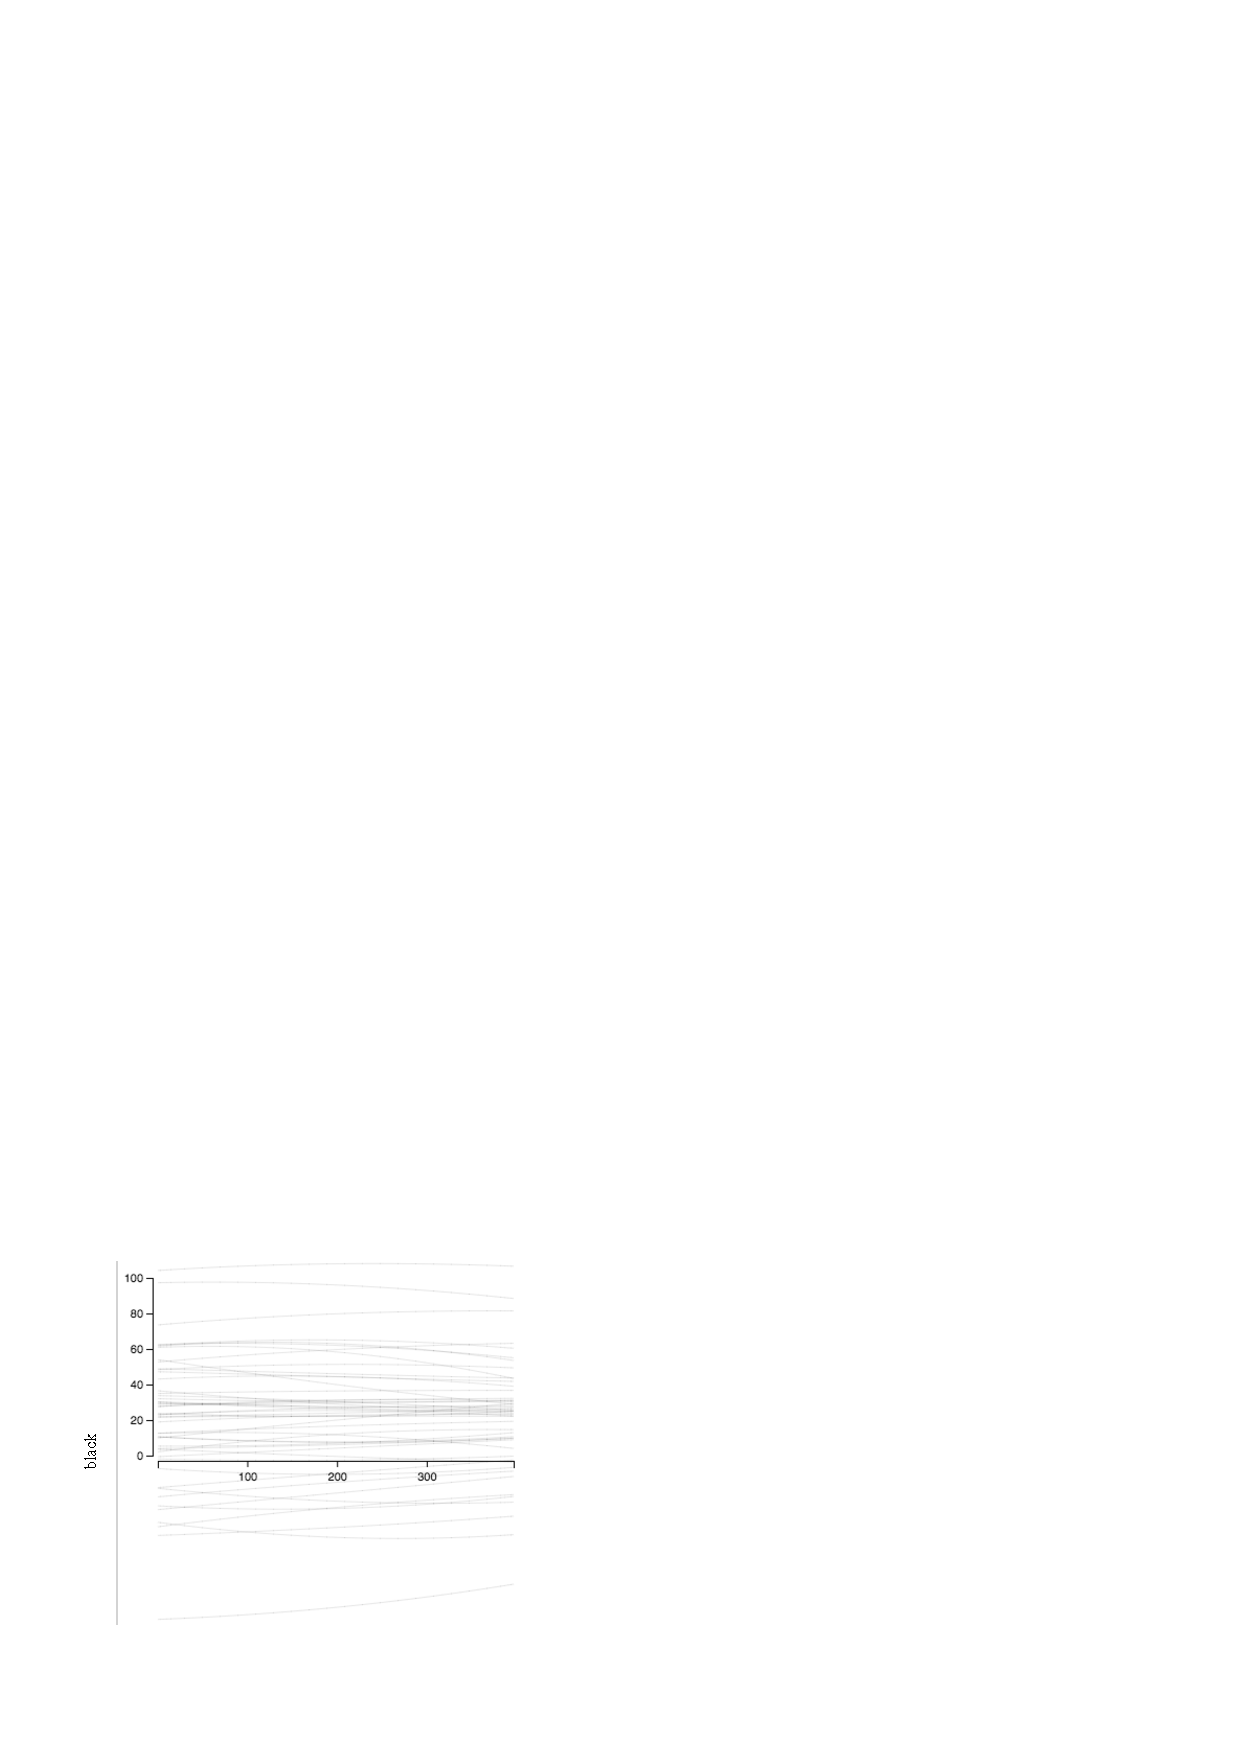
\includegraphics[width=\textwidth]{svmp_12.pdf}
    \end{subfigure}
    &
    \begin{subfigure}[b]{0.2\textwidth}
      \includegraphics[width=\textwidth]{nn5x3_12.pdf}
    \end{subfigure}
    &
    \begin{subfigure}[b]{0.2\textwidth}
      \includegraphics[width=\textwidth]{svmr_12.pdf}
    \end{subfigure}
    \\
    \hline \\
    \% lower status of the population &
    \begin{subfigure}[b]{0.2\textwidth}
      \includegraphics[width=\textwidth]{nn26_13.pdf}
    \end{subfigure}
    &
    \begin{subfigure}[b]{0.2\textwidth}
      \includegraphics[width=\textwidth]{svmp_13.pdf}
    \end{subfigure}
    &
    \begin{subfigure}[b]{0.2\textwidth}
      \includegraphics[width=\textwidth]{nn5x3_13.pdf}
    \end{subfigure}
    &
    \begin{subfigure}[b]{0.2\textwidth}
      \includegraphics[width=\textwidth]{svmr_13.pdf}
    \end{subfigure}
    \\
    \hline \\
  \end{tabular}
  }
\end{table}


